%%%%%%%%%%%%%%%%%%%%%%%%%%%%%%%%%%%%%%%%%%%%%%%%%%%%%%%%%%%%%%%%%%%%%%%%%%%%%%%
%%%  Plantilla para la elaboración del informe final de memorias de título  %%%
%%%  Adaptada por Oliver Diego Antonio Alarcón                              %%%
%%%%%%%%%%%%%%%%%%%%%%%%%%%%%%%%%%%%%%%%%%%%%%%%%%%%%%%%%%%%%%%%%%%%%%%%%%%%%%%

\documentclass[12pt,twoside]{report}
\usepackage[utf8]{inputenc}
\usepackage[spanish,es-tabla]{babel}
\usepackage[inner=2.5cm,outer=2cm,top=2.5cm,bottom=2cm]{geometry}
\usepackage{amsmath, amsfonts, amssymb}
\usepackage{graphicx, float}
\usepackage{subcaption}
\usepackage{booktabs}
\usepackage{longtable}
\usepackage{enumitem}
\usepackage{adjustbox}
\usepackage{makecell}
\usepackage{hyperref}
\usepackage{xcolor}
\usepackage{titlesec}
\usepackage{setspace}
\usepackage{svg}
\usepackage{float}
\usepackage{rotating}
\usepackage{todonotes}
\graphicspath{{images/}}

\setlength{\parindent}{12pt}
\titleformat{\chapter}
{\bfseries\large}{\chaptertitlename~\thechapter. }{0pt}{}
\titleformat{\section}
{\bfseries\large}{\thesection. }{0pt}{}

\begin{document}
\pagestyle{empty}

%%%%%%% Portada (Anexo C)
\begin{titlepage}
    \includegraphics[height=55pt]{escudoUdec}
    \begin{minipage}[b][60pt][c]{70ex}
    	\bfseries
        UNIVERSIDAD DE CONCEPCIÓN\\
        FACULTAD DE INGENIERÍA\\
        DEPARTAMENTO DE INGENIERÍA INFORMÁTICA\\
        Y CIENCIAS DE LA COMPUTACIÓN
    \end{minipage}
    \vspace{3cm}
    
    \begin{center}	
        \uppercase{\large\textbf{Uso De Estructuras De Datos Compactas Para Visualización De Series De Tiempo}}

        \vspace{1.5cm}
        POR
        \bigskip

        \textbf{Oliver Diego Antonio Brito Alarcón}

        \vspace{2cm}
        {\small Memoria de Título presentada a la Facultad de Ingeniería de la Universidad de Concepción para\\
        optar al título profesional de Ingeniero Civil Informático}
	
        \vspace{2cm}	
        \textbf{Profesores Guía} \\
        \bigskip
        
        José Fuentes \\
        Gonzalo Rojas


        \vfill
        Julio 2025

        Concepción (Chile)
        
        \bigskip
        \textcopyright{}
        2025 Oliver Diego Antonio Alarcón
	\end{center}
\end{titlepage}

%%%%%%%% Copyright
\textcolor{white}{.}
\vfill
\noindent\textcopyright{}
2025 Oliver Diego Antonio Alarcón\\
Se autoriza la reproducción total o parcial, con fines académicos, por cualquier medio o procedimiento, incluyendo la cita bibliográfica del documento.

%%%%% Dedicatoria
\clearpage
\onehalfspace
\vspace*{5cm}
\begin{flushright}
	A quienes el destino me dio por familia y a quienes la vida me permitió elegir como tal.
\end{flushright}

%%%%% Agradecimientos
\chapter*{Agradecimientos}
\thispagestyle{empty}
Esta Memoria de Título fue posible gracias al apoyo invaluable de mi madre, mi hermano y mi pareja, quienes estuvieron a mi lado y me permitieron concentrarme cuando más lo necesitaba.

A mis abuelos, gracias por su cariño y fortaleza. Y a mis amigues, gracias por su escucha, su compañía y por ayudarme a no perder la cordura durante esta etapa.
%%%%% Resumen
\clearpage
\pagestyle{plain}
\pagenumbering{roman} 
\chapter*{Resumen}
El creciente volumen de datos en aplicaciones modernas ha generado la necesidad de técnicas eficientes para su almacenamiento, análisis y visualización. Esta memoria explora el uso de estructuras de datos compactas —como \texttt{enc\_vector}, \texttt{vlc\_vector} y \texttt{dac\_vector} de la biblioteca \texttt{SDSL}— para representar series de tiempo de gran tamaño, combinándolas con algoritmos de \textit{downsampling} que permiten visualizar grandes volúmenes de información sin perder interpretabilidad. Se implementa una biblioteca en Python, \texttt{cv\_visualization}, que actúa como capa de compatibilidad entre estas estructuras y librerías de visualización como \texttt{Plotly}, \texttt{Altair} y \texttt{PyGal}.

Se diseñan experimentos para evaluar el impacto de estas técnicas en el uso de memoria durante la visualización (es decir, cuánta memoria RAM es necesario asignar en tiempo de ejecución), el tiempo de renderizado y el espacio de almacenamiento ocupado por los datos una vez reducidos. El análisis teórico y empírico incluye explicaciones detalladas de los esquemas de codificación utilizados, su complejidad de acceso y la comparación entre representaciones tradicionales y compactas.

Los resultados demuestran que, si bien el \textit{downsampling} mejora la velocidad de visualización, el uso de estructuras compactas puede sacrificar parcialmente esa velocidad —aunque sigue siendo menor que la necesaria para visualizar los datos originales—, y reduce en gran medida el espacio que ocupan los datos downsampleados en disco. Se mantiene la fidelidad visual de las gráficas, pero se identifican como limitaciones que algunas bibliotecas de visualización no son completamente compatibles con estas estructuras, ya que pueden descomprimir los datos de forma interna, provocando que el uso de memoria en tiempo de ejecución aumente significativamente y limite los beneficios esperados.

No quedan claros cuáles son los beneficios logrados con el trabajo, más allá de las limitaciones.

\chapter*{Abstract}
The growing volume of data in modern applications has created the need for efficient techniques for storage, analysis, and visualization. This thesis explores the use of compact data structures —such as \texttt{enc\_vector}, \texttt{vlc\_vector}, and \texttt{dac\_vector} from the \texttt{SDSL} library— to represent large time series, combining them with \textit{downsampling} algorithms that allow the visualization of massive datasets without losing interpretability. A Python library, \texttt{cv\_visualization}, was developed to serve as a compatibility layer between these structures and visualization libraries such as \texttt{Plotly}, \texttt{Altair}, and \texttt{PyGal}.

Experiments were designed to evaluate the impact of these techniques on memory usage during visualization (i.e., how much RAM needs to be allocated at runtime), rendering time, and the storage space occupied by the reduced datasets. Theoretical and empirical analysis includes detailed explanations of the encoding schemes used, their access complexity, and the comparison between traditional and compact representations.

The results show that while \textit{downsampling} improves visualization speed, the use of compact structures may partially sacrifice that speed—although it remains lower than rendering the original data—and significantly reduces the disk space occupied by downsampled datasets. Visual fidelity is preserved, but a notable limitation is that some visualization libraries are not fully compatible with these structures, as they may internally decompress the data, causing runtime memory usage to increase substantially and limiting the expected efficiency benefits.

%%%%% Índices
\tableofcontents
\listoftables
\listoffigures

%%%%% Cuerpo principal
\clearpage
\pagenumbering{arabic}

\section{Introducción}
\subsection{Contexto General}

Dar forma gráfica a la información es una herramienta valiosa, permitiendo que la misma sea más fácil y rápida de entender, comunicar e incluso aprender. 

Algo tan simple como analizar manualmente los registros de un sistema o sensor—lo cual puede requerir una cantidad considerable de tiempo para comprender qué ocurrió en un determinado día o a una hora específica—, puede graficarse como una serie de tiempo y permitir que ese análisis se haga en cuestión de segundos.

Todo esto es posible gracias a la \textbf{visualización}, que para efectos de esta Memoria de Título podemos entender como el uso de representaciones visuales interactivas, asistidas por computadora, para ayudar a la cognición.~\cite{card1999readings}. 

A pesar de esta definición, que posiciona la visualización como una herramienta que sienta sus bases en la computación, sus orígenes no se alinean con la llegada de la tecnología moderna. El adagio "Una imagen vale más que mil palabras", atribuida al dramaturgo y poeta Henrik Johan Ibsen, demuestra cómo esta idea se sienta en el imaginario colectivo como una verdad lógica. Incluso remontándonos a tiempos previos a nuestra era, las civilizaciones tempranas utilizaron distintos métodos para representar datos de forma visual, como el mapa estelar de Suzhou de la dinastía Song en China, que mostraba 1.434 estrellas agrupadas en 280 constelaciones~\cite{bonnetbidaud2009dunhuang}. Este y otros ejemplos históricos nos demuestran el deseo humano de centrar sus esfuerzos en simplificar información compleja en formas comprensibles y accesibles, utilizando representaciones visuales que potencian nuestra capacidad para observar patrones, relaciones y significados que de otro modo pasarían desapercibidos.

Este concepto es aún más prevalente en los tiempos que corren, ya que la llegada de las computadoras y el software ha revolucionado nuestra capacidad de manejar la información. Es gracias a estos avances tecnológicos que podemos analizar grandes volúmenes de información compleja, que normalmente no podríamos haber procesado sin la aparición de software específico para este objetivo. Nos referiremos a este tipo de datos como \textbf{Macrodatos} o \textbf{Big Data}\cite{mcafee2012bigdata}.

\subsubsection{Big Data}

La definición de \textit{Big Data} corresponde a la información de gran volúmen, gran velocidad y gran variedad que requiere formas innovadoras y eficientes para su procesamiento. Sin embargo, este término se popularizó al rededor del año 2012~\cite{diebold2012bigdata}, y lo que se consideraba \textit{Big Data} en el pasado es de mucha menor magnitud de lo que se considera hoy en día. Así mismo, la magnitud de estos datos en un futuro será mayor, ya que las capacidades de almacenamiento y procesamiento aumentarán.

Por tanto, se considerarán algunas características esenciales para asegurarnos de que estamos lidiando con macrodatos.
\begin{enumerate}
    \item \textbf{Variedad}: \\
        El conjunto de datos es heterogéneo, y normalmente no posee una estructura concreta para su procesamiento de manera nativa.
    \item \textbf{Velocidad}: \\
        Se refiera a la rapidez con la que los datos se generan. Normalmente los tipos de datos a analizar están en tiempo real, y generan nuevos datos a una frecuencia alta.
    \item \textbf{Volumen}: \\
        La cantidad de datos es significativa para el sistema donde se está trabajando y la tecnología actual.
\end{enumerate}

Otra característica importante a considerar de esta definición, es que estos datos son \textbf{inútiles} por sí solos,~\cite{gandomi2015beyond} la relevancia de este gran volúmen de información proviene del conjunto de \textbf{todos} los datos y la \textbf{interpretación} de los mismos. 

Al representar visualmente, por ejemplo, una serie de tiempo, es necesario acceder a cada uno de los elementos contenidos en el conjunto de datos para construir la gráfica correspondiente. Supongamos que disponemos de una secuencia de \( n \) puntos ordenados \((x_1, y_1), (x_2, y_2), \ldots, (x_n, y_n)\), los cuales deben ser procesados por el motor de renderizado de la herramienta de visualización. Este proceso conlleva, en el mejor de los casos, una complejidad temporal \(\mathcal{O}(n)\), ya que se requiere al menos una operación por cada punto para construir su representación gráfica.

Este comportamiento lineal implica que el tiempo necesario para renderizar una visualización crece proporcionalmente con la cantidad de datos. Por ejemplo, en la Figura~\ref{add_trace_plotly} se observa cómo la visualización de una serie de aproximadamente 350 mil puntos requiere cerca de 1.5 segundos para ser completada. Este tiempo, aunque aparentemente breve, resulta considerable en escenarios donde se espera interacción fluida, como el análisis exploratorio o los tableros de monitoreo en tiempo real.

\begin{figure}
    \centering
    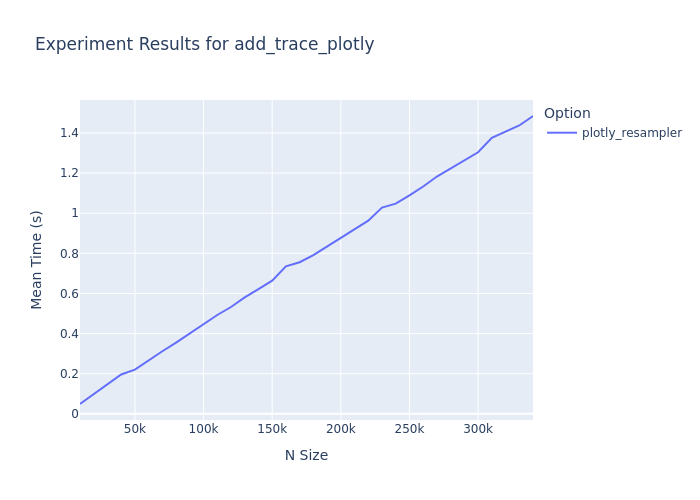
\includegraphics[width=0.9\linewidth]{introduction/images/add_trace_plotly.png}
    \title{figure}
    \caption{Tiempo promedio en segundos de graficar N cantidad de puntos usando la librería plotly.}
    \label{add_trace_plotly}
\end{figure}

De acuerdo con el informe publicado por Visa en 2017~\cite{visa2017facts}, su plataforma global de pagos posee la capacidad de procesar hasta 65{,}000 transacciones por segundo en condiciones de carga máxima. Sin embargo, en escenarios de uso más comunes, el volumen de transacciones tiende a rondar las 2{,}000 por segundo. Si consideramos un análisis retrospectivo de un solo día completo, el volumen total de datos asciende a un intervalo entre aproximadamente \(2{,}000 \times 86{,}400 = 1.728 \times 10^8\) (uso bajo) y \(65{,}000 \times 86{,}400 = 5.616 \times 10^9\) (uso máximo) transacciones por día.

Bajo este escenario, un trabajador que requiera analizar la actividad completa de un solo día enfrentaría una carga de datos que oscila entre cientos de millones y varios miles de millones de registros. Si asumimos un proceso de visualización con complejidad temporal \(\mathcal{O}(n)\), incluso los enfoques más optimizados en términos de eficiencia enfrentarán tiempos de procesamiento significativos y haciendo inviable su análisis oportuno.

Además del rendimiento, cuando trabajamos con series temporales extremadamente densas o con puntos altamente consecutivos entre sí, obtenemos gráficos difíciles de interpretar visualmente. Este problema genera la impresión de gráficos comprimidos o saturados ("squashed"), dificultando enormemente su cognición, como puede observarse claramente en la Figura \ref{squashed_plot}, que representa la lectura de un sensor colocado en un puente.

El creciente volumen de datos en contextos de Big Data nos obliga a repensar los fundamentos mismos de la visualización. Si graficar cientos de miles de puntos ya representa un reto técnico y cognitivo, ¿qué ocurre cuando nos enfrentamos a millones o incluso miles de millones de registros? En estos casos, la visualización deja de ser una simple representación directa de los datos y se transforma en un proceso de síntesis y decisión: ¿qué se debe mostrar, qué se puede omitir, y cómo evitar distorsionar la información en el camino?

\subsubsection{Downsampling}

Mejorar la eficiencia de los procesos que permiten la visualización es una manera de reducir los tiempos de cómputo, pero existen millones de escenarios donde esto no es suficiente. Aún con estas mejoras, llega una cantidad de puntos que simplemente no es viable visualizar en un tiempo prudente. Así mismo, la legibilidad de los gráficos no se resuelve con estos avances.

Es complejo escapar de esta problemática, ya que no podemos reducir la complejidad temporal lineal a menos que \textbf{no grafiquemos todos los puntos}.

Bajo esa idea surge la técnica conocida como \textit{downsampling}, la cual consiste en seleccionar solo un subconjunto de los puntos originales para ser graficados. A diferencia de métodos que generan nuevos datos mediante agregaciones o promedios, el \textit{downsampling} busca preservar puntos existentes del conjunto original que sean representativos de su comportamiento general. Su objetivo no es reemplazar el análisis detallado, sino facilitar la interpretación visual de grandes volúmenes de datos en contextos donde mostrar todos los puntos no es viable ni útil~\cite{steinarsson2013downsampling}. Esta técnica permite reducir el tiempo de renderizado y evitar la saturación visual sin comprometer, en teoría, la percepción de patrones relevantes. No obstante, su aplicación exige un criterio claro: ¿qué puntos se deben conservar para que la visualización siga siendo fiel a los datos?

Este acercamiento permite mejorar el rendimiento y la legibilidad sin comprometer significativamente la percepción de patrones relevantes. Existen múltiples algoritmos diseñados con este fin, los cuales serán analizados en detalle en la sección de Evaluación de Alternativas\ref{alternatives}.

\squashedplot
\downsample

El grupo de investigación \textbf{PreDiCT.IDLab}, afiliado a la Universidad de Gante en Bélgica, ha desarrollado e investigado activamente métodos avanzados para la visualización eficiente de series de tiempo. Entre sus contribuciones destaca la herramienta tsdownsample, un conjunto de algoritmos de alto rendimiento diseñados específicamente para realizar downsampling en contextos de visualización~\cite{tsdownsample}, la cual implementa los algoritmos ya mencionados para ser utilizados en \textit{python}.

Otra biblioteca de gran utilidad creada por estos académicos es \textit{plotly-resampler}~\cite{plotly-resampler}, la cual integra \textit{tsdownsample} de manera directa en \textit{plotly}. A pesar de el preprocesamiento necesario para generar una submuestra de una serie de tiempo, aún así podemos ver diferencias significativas en el tiempo necesario para la visualización de conjuntos grandes de información.

Esta mejora es evidente en la Figura \ref{plotly_vs_resampler}, donde podemos observar cómo usar \textit{plotly-resampler} disminuye el tiempo de ejecución al visualizar un conjunto de pares ordenados, a pesar de que es un \textit{wrapper} de \textit{plotly} y procesa el vector original. Esto se debe a que la cantidad de puntos seleccionados $(n_{out})$ es constante, por lo que la complejidad de crear un gráfico con técnicas de \textit{downsample} es $\mathcal{O}(n_{out})$, o sea, $\mathcal{O}(1)$.

\plotlyresampler

En definitiva, usar estrategias de \textit{downsample} es una opción muy útil a la hora de visualizar una serie de tiempo con muchos puntos, ya que permite mejorar la legibilidad, tiempo de renderización y, a causa de esto, el análisis de los datos que se están estudiando.

\subsection{Presentación del Problema}

A pesar de todas las ventajas que ofrece el uso de técnicas de \textit{downsampling} —como la mejora en el tiempo de renderizado, la reducción de la sobrecarga cognitiva y una experiencia más fluida al visualizar datos densos—, estas no necesariamente abordan todos los aspectos posibles de optimización dentro del proceso de visualización de series de tiempo.

Por ejemplo, herramientas como \textit{tsdownsample} permiten reducir la cantidad de puntos a representar, generando así gráficos más livianos y veloces. Sin embargo, incluso los datos ya reducidos siguen representándose con estructuras estándar que pueden ocupar un espacio considerable en memoria. En otras palabras, se reduce la cantidad de información a procesar, pero no necesariamente el tamaño de esa información en términos de espacio ocupado.

Esto plantea una nueva dimensión del problema: si ya hemos logrado disminuir significativamente el tiempo requerido para visualizar datos, ¿por qué no aprovechar esa mejora para optimizar también el espacio que ocupan los datos resultantes? Es decir, en lugar de mantenernos solo en la reducción de puntos, podríamos buscar formas de representar esa información de manera más eficiente, reduciendo aún más el tamaño total ocupado sin perder la capacidad de analizarla visualmente.

Un enfoque inicial para abordar esta problemática consiste en emplear \textbf{estructuras de datos compactas} con el objetivo de reducir aún más el espacio requerido para almacenar los datos visualizados. No obstante, estas estructuras presentan limitaciones importantes: muchas de ellas no permiten representar números flotantes, negativos e incluso, en algunos casos, el valor cero, lo que restringe su aplicabilidad en escenarios donde los datos numéricos presentan mayor diversidad.

Esta inquietud conduce a la exploración de técnicas adicionales de representación que, incluso a costa de un ligero incremento en el tiempo de cómputo (que ya se ha reducido en su complejidad), permitan disminuir de manera significativa el espacio ocupado por los datos. El objetivo es integrar estas estrategias de forma complementaria con los métodos de \textit{downsampling} existentes, logrando así un equilibrio más eficiente entre el rendimiento temporal y la optimización espacial.



\section{Objetivos del Proyecto}

El objetivo general de esta memoria es investigar si el uso de estructuras de datos compactas permite optimizar la visualización de series de tiempo de alta densidad, considerando tanto el rendimiento como la eficiencia en el uso del espacio.

\subsection{Objetivos Específicos}
\begin{enumerate}
\item Desarrollar herramientas que permitan evaluar el rendimiento y el uso de memoria durante la visualización de conjuntos de datos de gran tamaño.
\item Analizar el equilibrio entre uso de espacio y rendimiento al emplear estructuras de datos compactas en distintas etapas del proceso de downsampling.
\end{enumerate}


\section{Evaluación de Alternativas}
\label{alternatives}

\subsection{Técnicas de Downsampling}

Una vez introducido el concepto de downsampling como solución al problema de visualización de series de tiempo muy densas, es necesario revisar y comparar las principales alternativas existentes.

Diversos autores han propuesto algoritmos que permiten seleccionar los puntos más representativos de una serie para facilitar su visualización. A continuación, se presenta un resumen de los métodos más relevantes:

\begin{enumerate}
    \item \textbf{Mode-Median-Bucket (MMB)}: 
    Divide los datos en bloques y selecciona un punto por bloque usando la moda o la mediana de los valores. Es simple y fácil de entender, pero tiende a omitir picos y valles locales relevantes~\cite{steinarsson2013downsampling}.

    \item \textbf{Min-Std-Error-Bucket (MSEB)}: 
    Utiliza regresión lineal para calcular el error estándar entre pares de puntos, eligiendo aquellos que minimizan la suma de errores. Produce resultados estadísticamente coherentes, pero suaviza demasiado la serie y elimina detalles visuales importantes~\cite{steinarsson2013downsampling}.

    \item \textbf{Longest-Line-Bucket (LLB)}: 
    Similar a MSEB, pero en lugar de minimizar el error, maximiza la longitud total de las líneas entre puntos seleccionados. Tiene mejor capacidad para conservar picos extremos y fluctuaciones relevantes~\cite{steinarsson2013downsampling}.

    \item \textbf{Largest-Triangle-Three-Buckets (LTTB)}: 
    Divide los datos en tres bloques consecutivos y selecciona el punto que forma el triángulo de mayor área con los puntos de los bloques adyacentes. Esta técnica preserva bien la forma general del gráfico y es eficiente computacionalmente~\cite{steinarsson2013downsampling}.

    \item \textbf{Largest-Triangle-Dynamic (LTD)}: 
    Variante del LTTB que adapta dinámicamente el tamaño de los bloques según la variación local de los datos. Mejora la representación visual en series con regiones muy fluctuantes y otras más estables~\cite{steinarsson2013downsampling}.

    \item \textbf{MinMaxLTTB}: 
    Propuesto por Van Der Donckt et al.~\cite{vanderdonckt2023minmaxlttb}, este algoritmo mejora la escalabilidad de LTTB al aplicar una preselección eficiente de puntos mínimos y máximos verticales mediante el algoritmo MinMax, para luego aplicar LTTB solo sobre esos puntos seleccionados. De esta manera, reduce significativamente el tiempo de cómputo sin sacrificar calidad visual.
\end{enumerate}

Dado el enfoque de este trabajo, se seleccionó principalmente el uso del algoritmo \textbf{MinMaxLTTB}. Esta decisión se fundamenta en varios factores: en primer lugar, el algoritmo ha sido propuesto por los mismos autores que desarrollaron la biblioteca \texttt{tsdownsample}, lo que garantiza una implementación de referencia optimizada y bien documentada. Además, MinMaxLTTB presenta un excelente equilibrio entre rendimiento y fidelidad visual, al combinar una reducción sustancial en el tiempo de cómputo con una buena preservación de la forma general de la serie de tiempo.

Como complemento para el análisis comparativo, también se utilizará el algoritmo \textbf{LTTB}, ya que es ampliamente citado en la literatura como una opción base eficiente, y su comparación directa con MinMaxLTTB permite observar el impacto de la estrategia de preselección aplicada por los autores.

\subsection{Estructuras de Datos Compactas}

El uso de estructuras de datos compactas permite representar secuencias numéricas en memoria utilizando una menor cantidad de bits por elemento, manteniendo el acceso a los datos sin pérdida de información. 

Para uso de este tipo de estructuras, se utiliza la biblioteca \texttt{sdsl4py}, un conjunto de bindings en Python para la Succinct Data Structure Library (SDSL), que permite acceder a múltiples representaciones comprimidas desde entornos de análisis como Python. A continuación se presentan las principales estructuras disponibles en \texttt{sdsl4py}.

\begin{enumerate}
    \item \textbf{enc\_vector\_elias\_gamma}:
    Utiliza codificación de enteros Elias-Gamma. Es eficiente para valores pequeños, ya que su tamaño codificado crece logarítmicamente con el valor. No puede representar ceros.

    \item \textbf{enc\_vector\_elias\_delta}:
    Variante de Elias-Gamma que mejora la compresión para valores grandes, manteniendo eficiencia en lectura. También requiere que todos los valores sean mayores que cero.

    \item \textbf{enc\_vector\_fibonacci}:
    Usa codificación basada en la sucesión de Fibonacci. Esta técnica es compacta y libre de prefijos, pero tiene limitaciones para valores cero y una complejidad levemente mayor en decodificación.

    \item \textbf{enc\_vector\_comma\_2}:
    Codificación por comas binarias (comma-2), una forma simple y eficiente de codificar enteros con separación de bits mediante una secuencia especial. Ofrece buena compresión para secuencias no muy dispersas.

    \item \textbf{vlc\_vector\_elias\_delta}:
    Variante del enc\_vector\_elias\_delta que permite acceso más rápido a los elementos gracias a una estructura de lectura optimizada (Variable-Length Codes con índice de acceso directo).

    \item \textbf{vlc\_vector\_elias\_gamma}:
    Equivalente a la anterior, pero usando codificación Elias-Gamma. Útil cuando se prioriza el acceso sobre la compresión máxima.

    \item \textbf{vlc\_vector\_fibonacci}:
    Combina las ventajas de codificación Fibonacci con accesos más eficientes mediante índices auxiliares.

    \item \textbf{vlc\_vector\_comma\_2}:
    Aplica codificación comma-2 con estructura de acceso rápido. Es útil cuando se necesita acceder a datos comprimidos con latencias bajas.

    \item \textbf{dac\_vector}:
    Utiliza Directly Addressable Codes (DAC), una estructura escalonada que permite un buen balance entre compresión y velocidad de acceso. Es especialmente útil para secuencias de enteros donde los valores tienen alta varianza.

\end{enumerate}

Como podemos apreciar en el Anexo~\ref{anexo_sdsl4py}, al evaluar la velocidad de acceso, el tiempo de construcción y el espacio utilizado por las distintas alternativas de estructuras de datos compactas, no se observa una diferencia significativa en cuanto a su curva de complejidad teórica. No obstante, para determinar cuál estructura resulta más adecuada en la práctica, se define una \textbf{relación compuesta} que pondera las tres métricas principales.

Esta relación se formula como:

\begin{equation}
\text{Score}(E) = \alpha \cdot \text{AccessTime}(E) + \beta \cdot \text{BuildTime}(E) + \gamma \cdot \text{SpaceUsed}(E)
\end{equation}

donde:
\begin{itemize}
    \item $E$ representa una estructura evaluada,
    \item $\text{AccessTime}(E)$, $\text{BuildTime}(E)$ y $\text{SpaceUsed}(E)$ corresponden a los valores empíricos medidos para dicha estructura,
    \item y $\alpha$, $\beta$, y $\gamma$ son coeficientes de ponderación tales que $\alpha + \beta + \gamma = 1$.
\end{itemize}

Estos coeficientes pueden ser ajustados en función de los objetivos específicos del sistema o aplicación. Por ejemplo, en un entorno donde el rendimiento en lectura sea prioritario, se puede asignar un valor mayor a $\alpha$; en cambio, si se trabaja con recursos de almacenamiento limitados, se puede incrementar el peso de $\gamma$. 

En esta ocasión, se consideran los valores:

\begin{itemize}
    \item $\alpha = 0.6$
	\item $\beta = 0.4$
	\item $\gamma = 0.3$
\end{itemize}

\begin{table}[H]
\centering
\caption{Puntaje promedio por estructura (menor es mejor)}
\label{tab:score_promedio_estructuras}
\begin{tabular}{l r}
\toprule
\textbf{Estructura} & \textbf{Score promedio} \\
\midrule
vlc\_vector\_elias\_delta - 8 & 204.200 \\
vlc\_vector\_elias\_gamma - 8 & 218.200 \\
vlc\_vector\_comma\_2 - 8     & 231.800 \\
dac\_vector - 8              & 232.600 \\
No Compression - 8           & 1776.000 \\
\bottomrule
\end{tabular}
\end{table}

A partir de la puntuación resultante, se seleccionan las estructuras de datos \textit{vlc\_vector\_elias\_delta} por ser la de mejor puntuación, y \textit{dac\_vector} por ser la siguiente estructura con buen rendimiento, pero que además representa una técnica de compresión distinta, basada en \textit{Directly Addressable Codes}. Esta elección permite contrastar dos enfoques diferentes de compresión (códigos de longitud variable vs. esquemas direccionables) y evaluar su impacto práctico en la visualización de datos comprimidos.

\section{Desarrollo}


\subsection{Uso de \texttt{sdsl4py} para la visualización de datos}

La biblioteca \texttt{sdsl4py} expone en Python diversas estructuras de datos compactas de la librería \texttt{sdsl-lite}, diseñada originalmente para representar secuencias de enteros sin signo de forma eficiente en términos de espacio. El flujo de trabajo básico consiste en construir un \texttt{int\_vector} modificable con un tamaño predefinido, cargar los datos en él, y luego aplicar una estrategia de compresión específica. Una vez comprimido, el vector pasa a ser de solo lectura.

Aunque estas estructuras pueden integrarse con bibliotecas como \texttt{plotly}, presentan una limitación clave: no admiten valores flotantes ni negativos de forma nativa. Esto se debe a que las técnicas de compresión empleadas —como las codificaciones de Elias o Fibonacci— asumen enteros positivos, donde patrones de repetición o crecimiento logarítmico pueden ser aprovechados para reducir el espacio.

Cuando se trabaja con series de tiempo u otros datos con decimales, la representación compacta se vuelve más compleja. Los valores flotantes tienden a carecer de regularidad en su representación binaria, dificultando la compresión efectiva. Además, representar signos o fracciones dentro de estructuras diseñadas exclusivamente para enteros sin signo requiere soluciones externas, como escalado previo o codificaciones personalizadas, que introducen sobrecarga adicional y limitan la interoperabilidad con los algoritmos ya existentes.

Por estas razones, aunque \texttt{sdsl4py} puede ser útil para visualizar datos discretos o transformados a enteros, no resulta una opción directa ni eficiente para representar valores reales sin una etapa de preprocesamiento.


\subsection{CompressedVector}

Para superar la limitación de que \texttt{sdsl4py} sólo permite almacenar enteros sin signo (\textit{uint}), se propone una estructura llamada \texttt{CompressedVector}, que habilita la representación de números reales (positivos, negativos y \texttt{NaN}) mediante la combinación de varias estructuras compactas para representar vectores de enteros,\texttt{int\_vector<>}. La estrategia consiste en descomponer cada número flotante en tres componentes separados:

\begin{enumerate}
    \item \textbf{Parte entera}: el valor absoluto truncado del número.
    \item \textbf{Parte decimal}: los decimales, escalados como enteros según la precisión deseada.
    \item \textbf{Indicador de signo}: codificación entera que distingue entre valores positivos, negativos y \texttt{NaN}.
\end{enumerate}

Dado un número real $x \in \mathbb{R}$ y una precisión de $d$ dígitos decimales, la transformación se define como:

\begin{align*}
    x &= \pm \left( \lfloor |x| \rfloor + \frac{\mathrm{decimales}(x)}{10^d} \right) \\
    \text{parte\_entera} &= \lfloor |x| \rfloor \\
    \text{parte\_decimal} &= \left\lfloor (|x| - \lfloor |x| \rfloor) \cdot 10^d \right\rfloor \\
    \text{signo} &=
        \begin{cases}
            1 & \text{si } x \geq 0 \\
            0 & \text{si } x < 0 \\
            2 & \text{si } x \text{ es } \texttt{NaN}
        \end{cases}
\end{align*}

Cada uno de estos componentes se almacena en un \texttt{int\_vector<>} distinto, lo que permite aplicar técnicas de compresión sobre los mismos.
\vspace{1em}
\noindent
Es posible recuperar la $i$-ésima entrada del vector original mediante la operación inversa:

\begin{align*}
    \text{si } \text{signo}[i] = 2, \quad &\Rightarrow x_i = \texttt{NaN} \\
    \text{sino: } \quad &x_i = (-1)^{1 - \text{signo}[i]} \cdot \left( \text{parte\_entera}[i] + \frac{\text{parte\_decimal}[i]}{10^d} \right)
\end{align*}

\noindent
Este procedimiento está implementado en el método \texttt{\_reconstruct\_float\_value} de la clase \texttt{CompressedVector}, y utiliza la biblioteca \texttt{Decimal} de Python para preservar la precisión durante las operaciones aritméticas.

\vspace{1em}
\noindent
Si bien esta solución requiere más espacio que una única estructura de datos compacta, permite una representación robusta y precisa de números reales, manteniendo las ventajas de compresión que ofrece \texttt{sdsl4py} para enteros.

Para facilitar su uso dentro del ecosistema Python y su interoperabilidad con bibliotecas estándar, \texttt{CompressedVector} implementa múltiples operaciones comunes mediante funciones mágicas (\textit{dunder methods}). En la siguiente tabla se resumen las principales funcionalidades disponibles.

\begin{table}[H]
\centering
\renewcommand{\arraystretch}{1.3} % Aumenta la altura de las filas de forma consistente
\begin{tabular}{|p{3.5cm}|p{6cm}|p{5cm}|}
\hline
\textbf{Operación} & \textbf{Descripción} & \textbf{Método implementado} \\
\hline
\rule{0pt}{1.5em}Indexación         & Acceso a un elemento por índice                & \texttt{\_\_getitem\_\_(index)} \\
\hline
\rule{0pt}{1.5em}Asignación         & Modificación de un valor en un índice dado     & \texttt{\_\_setitem\_\_(index, value)} \\
\hline
\rule{0pt}{1.5em}Tamaño             & Cantidad de elementos almacenados              & \texttt{\_\_len\_\_()} \\
\hline
\rule{0pt}{1.5em}Iteración          & Permite iterar sobre los elementos             & \texttt{\_\_iter\_\_()} \\
\hline
\rule{0pt}{1.5em}Representación     & Muestra formato legible para impresión         & \texttt{\_\_repr\_\_()} \\
\hline
\rule{0pt}{1.5em}Suma               & Suma escalar a todos los elementos             & \texttt{\_\_add\_\_(other)} \\
\hline
\rule{0pt}{1.5em}Suma in-place      & Suma escalar modificando el vector             & \texttt{\_\_iadd\_\_(other)} \\
\hline
\rule{0pt}{1.5em}Resta              & Resta escalar a todos los elementos            & \texttt{\_\_sub\_\_(other)} \\
\hline
\rule{0pt}{1.5em}Resta in-place     & Resta escalar modificando el vector            & \texttt{\_\_isub\_\_(other)} \\
\hline
\rule{0pt}{1.5em}Multiplicación     & Multiplica todos los valores por escalar       & \texttt{\_\_mul\_\_(other)} \\
\hline
\rule{0pt}{1.5em}Multiplicación in-place & Multiplica modificando el vector         & \texttt{\_\_imul\_\_(other)} \\
\hline
\rule{0pt}{1.5em}División           & Divide todos los elementos por un escalar      & \texttt{\_\_truediv\_\_(other)} \\
\hline
\rule{0pt}{1.5em}División in-place  & Divide modificando el vector                   & \texttt{\_\_itruediv\_\_(other)} \\
\hline
\rule{0pt}{1.5em}Comparación        & Compara igualdad elemento a elemento           & \texttt{\_\_eq\_\_(other)} \\
\hline
\end{tabular}
\caption{Operaciones implementadas en la clase \texttt{CompressedVector}}
\end{table}

\subsection{CompressedVectorDownsampler}

Hasta ahora hemos abordado por separado el uso de estructuras de datos compactas y las técnicas de \textit{downsampling}. La clase \texttt{CompressedVectorDownsampler} combina ambos enfoques en una única solución, permitiendo obtener datos listos para ser graficados tras haber sido comprimidos y reducidos.

Esta clase integra internamente las funcionalidades de \texttt{CompressedVector} y \texttt{TsDownsample}. El usuario puede proporcionar como entrada uno o ambos vectores originales (\texttt{x} y \texttt{y}), junto con los siguientes parámetros:

\begin{itemize}
    \item Cantidad de decimales a conservar.
    \item Tamaño del entero a utilizar (8, 16, 32 o 64 bits).
    \item Método de compresión (como función o identificador en forma de \texttt{string}).
    \item Estrategia de \textit{downsampling} (también como función o \texttt{string}).
    \item Número deseado de puntos de salida (\texttt{n\_out}).
\end{itemize}

Como resultado, se obtienen los vectores \texttt{x} y/o \texttt{y} ya procesados, tanto por \textit{downsampling} como por compresión, permitiendo al usuario almacenar información densa en una fracción del espacio original. Esto garantiza una reducción significativa en el uso de almacenamiento y en los tiempos de renderización durante la visualización.


\subsection{Librerías de Visualización}

El propósito de esta sección es explorar cómo las herramientas desarrolladas en este trabajo pueden integrarse con bibliotecas de visualización ya existentes. No se contempla la creación de una nueva biblioteca gráfica, sino la adaptación y evaluación de las opciones disponibles para visualizar datos procesados mediante compresión y \textit{downsampling}.

A continuación, se presentan las bibliotecas consideradas en este estudio, agrupadas según su compatibilidad con las estructuras propuestas.

\subsubsection{Bibliotecas Dependientes de NumPy}

Muchas bibliotecas populares de visualización en Python, como \texttt{matplotlib}~\cite{matplotlib}, \texttt{plotly} y \texttt{plotly-resampler}, ofrecen amplias funcionalidades para construir gráficos interactivos y estáticos. Sin embargo, todas ellas presentan una limitación importante: requieren explícitamente que los datos de entrada sean arreglos de tipo \texttt{numpy.ndarray}, o bien realizan una conversión interna hacia dicho formato.

Esto representa una incompatibilidad con \texttt{CompressedVector}, ya que \texttt{numpy} impone restricciones sobre el tipo y tamaño de los elementos almacenados. En particular, requiere que todos los elementos de un arreglo tengan el mismo tamaño en bits (por ejemplo, \texttt{int32}, \texttt{float64}, etc.), lo que entra en conflicto con la propuesta de compresión variable y eficiente de \texttt{CompressedVector}, donde los elementos están representados internamente con diferentes esquemas de codificación.

Como consecuencia, al intentar visualizar los datos comprimidos directamente con estas bibliotecas, se hace necesario descomprimirlos previamente. Para ello, la clase \texttt{CompressedVector} ofrece la opción \texttt{get\_decompressed=True}, que entrega una representación expandida compatible con \texttt{numpy}. Sin embargo, este proceso elimina los beneficios de la compresión, incrementando significativamente la memoria alocada y desaprovechando las ventajas espaciales del enfoque.

Resolver esta limitación está fuera del alcance de este trabajo. Sería necesario modificar el código fuente de estas bibliotecas para aceptar iteradores genéricos sin forzar una conversión a \texttt{numpy}, o bien desarrollar un nuevo tipo de dato compatible con la infraestructura de \texttt{numpy}. Ambos caminos implican un esfuerzo considerable y una reestructuración profunda del ecosistema.

\subsubsection{PyGal}

\texttt{PyGal} es una biblioteca orientada a la generación de gráficos SVG embebibles para la web~\cite{pygal}. Aunque ofrece funcionalidades básicas como gráficos de líneas y dispersión, se destaca por una característica clave: acepta cualquier objeto iterable como fuente de datos, sin necesidad de convertirlo a \texttt{numpy}. Gracias a esto, \texttt{PyGal} es plenamente compatible con \texttt{CompressedVector} y \texttt{CompressedVectorDownsampler}.

No obstante, esta flexibilidad tiene un costo. \texttt{PyGal} presenta limitaciones notables en cuanto a interactividad y personalización. No permite acciones como zoom, selección dinámica de puntos o animaciones avanzadas, lo que restringe su utilidad en contextos donde el análisis visual requiere exploración activa y responsiva.

\subsubsection{Vega-Altair}

\texttt{Vega-Altair} es una biblioteca declarativa para la visualización de datos en Python, basada en la gramática de gráficos de \texttt{Vega-Lite}~\cite{altair}. Su API es coherente, legible y potente, permitiendo crear visualizaciones complejas con poco código.

Una de sus principales ventajas es su compatibilidad con estructuras iterables sin requerir conversión explícita a \texttt{numpy}. Esto la hace adecuada para trabajar directamente con \texttt{CompressedVectorDownsampler}, permitiendo visualizar datos comprimidos y downsampleados sin perder eficiencia espacial.

\texttt{Altair} combina muchas de las fortalezas de bibliotecas como \texttt{plotly} y \texttt{matplotlib}, ofreciendo soporte para múltiples tipos de gráficos, interactividad avanzada y buena integración con el ecosistema de análisis de datos en Python. Por estas razones, ha sido la herramienta principal utilizada en los experimentos de esta memoria y se recomienda como la opción preferente para trabajos futuros.


\subsection{Framework de Experimentación}
\label{benchmarking}
%aqui falta hilar un poco estas ideas...
Benchmarking es el proceso continuo de comparar el desempeño, productos o prácticas de una organización, sistema o componente con referentes externos —como líderes de la industria o soluciones de alto rendimiento— con el objetivo de identificar brechas y oportunidades de mejora. Este proceso no se limita sólo a la recolección de métricas, sino que también implica el análisis crítico y, cuando es pertinente, la adopción o adaptación de ideas y métodos que han demostrado ser eficaces.~\cite{stapenhurst2009benchmarking}

En el contexto de la Memoria de Título, el benchmarking se refiere a los experimentos definidos en el anexo\ref{sec:experimentos}, que evalúan distintos aspectos de la implementación propuesta: espacio, memoria, tiempo de renderización y construcción, entre otros.

Para ese objetivo, se desarrolló un framework de experimentación que se detalla en las subsecciones a continuación.

\subsubsection{Sacred}

Para llevar a cabo las comparaciones se utilizó la biblioteca \texttt{Sacred}, una herramienta de Python que permite configurar, organizar, registrar y reproducir experimentos computacionales~\cite{greff2017sacred}. Está diseñada para introducir una sobrecarga mínima, fomentando la modularidad y flexibilidad en su implementación.

Esta biblioteca permite ejecutar experimentos de forma estructurada, manteniendo control sobre los parámetros involucrados. Se definió una configuración base con parámetros comunes, pero cada experimento puede especificar valores propios que reemplazan a los generales cuando corresponde.

Por ejemplo, se estableció globalmente que cada experimento debe ejecutarse 100 veces, con el fin de obtener un promedio representativo. Sin embargo, en ciertos casos —como en las pruebas de espacio, donde los resultados son estables y no requieren repetición— este valor se reemplaza localmente por una sola ejecución. Así, mientras los ensayos de tiempo usan múltiples iteraciones por defecto, los de uso de espacio en disco se realizan solo una vez.

\subsubsection{Input Handler}

\textit{InputHandler} es una clase auxiliar que permite cargar datos desde archivos CSV y convertirlos en diferentes formatos, ya sea sin compresión, con compresión usando \textit{CompressedVector}, o bien aplicando técnicas de reducción de puntos. Su diseño parametrizable permite ajustar el formato de los datos para facilitar su uso en pruebas de benchmarking.

\vspace{0.5em}
\textbf{Configuración:} mediante el método \textit{set\_width()}, se puede definir el ancho de bits para la parte entera de los datos en los ejes \textit{x} e \textit{y}, lo que incide directamente en la eficiencia del almacenamiento comprimido.

\vspace{0.5em}
\textbf{Extracción de datos:} la función \textit{get\_from\_file()} permite cargar columnas desde archivos CSV, entregando los datos en distintos formatos según el parámetro \textit{option}:
\begin{itemize}
    \item \textit{"default"}: datos crudos en \textit{float}.
    \item \textit{"compressed\_vector"}: representación comprimida con \textit{CompressedVector}.
    \item \textit{"compressed\_vector\_downsampler"}: compresión + reducción usando \textit{CompressedVectorDownsampler}.
    \item \textit{"tsdownsample"}: reducción usando librería externa \textit{tsdownsample}.
\end{itemize}

\vspace{0.5em}
\textbf{Compresión:} el método interno \textit{compress\_vector()} se encarga de transformar una lista de valores en un \textit{CompressedVector}, aplicando las opciones de redondeo, compresión, y configuración de bits especificadas por el usuario.

\vspace{0.5em}
\textbf{Índices seleccionados:} luego de aplicar reducción, es posible recuperar los índices de los puntos seleccionados mediante \textit{get\_x\_indices()} y \textit{get\_y\_indices()}, lo que resulta útil para visualizar los puntos elegidos o analizar su distribución.

\subsubsection{Experiment Runner}

Llamamos \textit{Experiment Runner} a una serie de herramientas definidas en el benchmarking que nos permiten ejecutar cualquier experimento previamente definido. Este módulo gestiona las configuraciones globales, aplica los parámetros correspondientes a cada caso, ejecuta la función de evaluación y almacena los resultados mediante la librería \textit{Sacred} en un archivo \textit{.json}.

Por cada experimento, se registra la siguiente información:

\begin{itemize}
    \item \textit{option}: tipo de representación utilizada (ej. \textit{default}, \textit{compressed\_vector}, etc.).
    \item \textit{file}: nombre base del archivo de entrada.
    \item \textit{n\_size}: cantidad de datos utilizados en la muestra.
    \item \textit{n\_out}: tamaño de la salida en caso de reducción.
    \item \textit{mean}: promedio del valor medido en las iteraciones.
    \item \textit{stdev}: desviación estándar del valor medido.
    \item \textit{min} y \textit{max}: valores mínimo y máximo observados.
    \item \textit{all\_differences}: lista completa con los resultados individuales por iteración.
    \item \textit{iterations}: cantidad de veces que se repitió el experimento.
    \item \textit{measurement\_unit}: unidad de medida correspondiente (por ejemplo, milisegundos o bytes).
\end{itemize}

Estos datos permiten evaluar de forma cuantitativa el comportamiento de diferentes estrategias de compresión y visualización frente a distintos volúmenes de entrada.

Además de los resultados cuantitativos de cada experimento, el archivo \textit{.json} generado por \textit{Sacred} incluye información complementaria útil para trazabilidad y reproducibilidad. Por ejemplo, se registra el nombre del experimento, la ruta base de ejecución, las versiones exactas de las dependencias utilizadas, los archivos fuente involucrados, y metadatos del sistema donde se ejecutó (CPU, sistema operativo, versión de Python, etc.). También se incluyen los commits y estado del repositorio \textit{git}, permitiendo asociar los resultados directamente con una versión específica del código. Esta información permite contextualizar los resultados y asegurar que los experimentos puedan ser replicados en el futuro con fidelidad.

\subsubsection{Plantilla De Experimentos}

Dentro del repositorio, el archivo \textit{template.py} actúa como base para definir cualquier experimento compatible con el framework de benchmarking. Este archivo contiene una estructura mínima y parametrizable que permite registrar, configurar y ejecutar un experimento completo con la ayuda de \textit{Sacred}.

La estructura del experimento tiene tres componentes clave:

\begin{itemize}
    \item \textbf{Título del experimento:} definido mediante \textit{exp\_name}, permite organizar los resultados en carpetas separadas y legibles.
    \item \textbf{Configuración:} a través del decorador \textit{@exp.config} se definen los \textit{casos de prueba} (por ejemplo, vectores sin comprimir, comprimidos, o reducidos), así como el rango de tamaños de entrada y otros parámetros globales.
    \item \textbf{Función principal:} bajo el decorador \textit{@exp.automain}, se implementa la función que será ejecutada con los parámetros definidos. Esta instancia recibe una función \textit{experiment\_fn}, que representa la lógica específica del experimento (por ejemplo, medir tiempo de ejecución), y se conecta con el \textit{Experiment Runner} para la ejecución repetida, registro de métricas y almacenamiento de resultados.
\end{itemize}

Dentro de \textit{experiment\_fn(x, y, option)}, el usuario define lo que desea medir utilizando los datos entregados por el \textit{InputHandler}. Por ejemplo, se puede medir el tiempo de ejecución de un proceso sobre los datos \textit{x} e \textit{y}, o bien calcular la precisión de una reconstrucción. Este valor es luego devuelto al \textit{Experiment Runner}, que lo almacena junto con las configuraciones usadas.

Gracias a esta plantilla, definir nuevos experimentos se vuelve un proceso sencillo, flexible y reutilizable.
\section{Pruebas Sobre el Sistema}
\label{sec:pruebas-sistema}

Usando el framework descrito en la Sección~\ref{benchmarking}, se declararon distintos experimentos a partir de la plantilla base del repositorio. Cada uno de ellos evalúa distintos aspectos del sistema como el uso de memoria, tiempos de ejecución o el tamaño ocupado por diferentes representaciones de datos. La descripción de cada experimento, así como sus valores de entrada y salida se encuentran en el Anexo~\ref{anexo-resumen-experimentos}.

\subsection{Acceso en CompressedVector con Diferentes Decimales}
\label{exp:cvd-access-decimals}

% imagen
\begin{figure}[H]
    \centering
    
\includegraphics[width=0.8\textwidth]{testing/images/decimal_places_access.png}
    \caption{Resultados de los experimentos de acceso en CompressedVector con diferentes decimales de precisión.}
    \label{fig:cvd-access-decimals}
\end{figure}

Los resultados del experimento demuestran que el tiempo de acceso promedio por índice en un \texttt{CompressedVector}...


% \input{testing/altair-mem.tex}
\subsection{Asignación de Memoria en Todas las Librerías}
\label{exp:all-libs-mem}

\begin{figure}[H]
    \centering
    
\includegraphics[width=0.8\textwidth]{testing/images/all_libs_mem.png}
    \caption{Resultados del experimento: Asignación de Memoria en Todas las Librerías.}
    \label{fig:all-libs-mem}
\end{figure}

...

\subsection{Comparación de Espacio Usado por Representación}
\label{exp:space-comparison}

\begin{figure}[H]
    \centering
    
\includegraphics[width=0.8\textwidth]{img\space_comparison.png}
    \caption{Resultados del experimento: Comparación de Espacio Usado por Representación.}
    \label{fig:space-comparison}
\end{figure}

...

\subsection{Comparación de Tiempo de Compresión}
\label{exp:compression-time}

\begin{figure}[H]
    \centering
    
\includegraphics[width=0.8\textwidth]{img\compression_time.png}
    \caption{Resultados del experimento: Comparación de Tiempo de Compresión.}
    \label{fig:compression-time}
\end{figure}

...

\subsection{Comparación de Tiempos de Graficado en Todas las Librerías}
\label{exp:all-libs-time}

\begin{figure}[H]
    \centering
    
\includegraphics[width=0.8\textwidth]{testing/images/all_libs_time.png}
    \caption{Resultados del experimento: Comparación de Tiempos de Graficado en Todas las Librerías.}
    \label{fig:all-libs-time}
\end{figure}

...

\subsection{Construcción de CompressedVector con Diferentes Decimales}
\label{exp:cvd-build-decimals}

\begin{figure}[H]
    \centering
    
\includegraphics[width=0.8\textwidth]{testing/images/cvd_build_decimals.png}
    \caption{Resultados del experimento: Construcción de CompressedVector con Diferentes Decimales.}
    \label{fig:cvd-build-decimals}
\end{figure}

...

% \input{testing/cvd-sdsl-build.tex}
\subsection{Tamaño en Memoria de CompressedVector con Diferentes Decimales}
\label{exp:cvd-size-decimals}

\begin{figure}[H]
    \centering
    
\includegraphics[width=0.8\textwidth]{testing/images/cvd_size_decimals.png}
    \caption{Resultados del experimento: Tamaño en Memoria de CompressedVector con Diferentes Decimales.}
    \label{fig:cvd-size-decimals}
\end{figure}

...

\subsection{Tiempo Total de Construcción y Graficado con Altair}
\label{exp:altair-total-time}

\begin{figure}[H]
    \centering
    
\includegraphics[width=0.8\textwidth]{testing/images/altair_total_time.png}
    \caption{Resultados del experimento: Tiempo Total de Construcción y Graficado con Altair.}
    \label{fig:altair-total-time}
\end{figure}

...

\subsection{Tiempos de Graficado con Pygal}
\label{exp:pygal-time}

\begin{figure}[H]
    \centering
    
\includegraphics[width=0.8\textwidth]{img\pygal_time.png}
    \caption{Resultados del experimento: Tiempos de Graficado con Pygal.}
    \label{fig:pygal-time}
\end{figure}

...

\subsection{Tiempos de Graficado con Vega-Altair}
\label{exp:altair-time}

\begin{figure}[H]
    \centering
    
\includegraphics[width=0.8\textwidth]{img\altair_time.png}
    \caption{Resultados del experimento: Tiempos de Graficado con Vega-Altair.}
    \label{fig:altair-time}
\end{figure}

...

\section{Conclusiones}

El carácter de la Memoria de Título es principalmente experimental. Las herramientas desarrolladas durante su realización han servido para delimitar un esquema general del potencial respecto al uso de estructuras de datos compactas para la visualización de datos, centrándose en una visión general de los caminos posibles que se ramifican a partir de la investigación realizada y los resultados obtenidos.

El uso de estructuras de datos compactas para la visualización de datos es un campo en constante evolución, y los resultados obtenidos en esta Memoria de Título sugieren que hay un gran potencial para mejorar la eficiencia y la efectividad de las visualizaciones. A pesar de que éstas no han sido implementadas para su uso con valores flotantes, el desarrollo de la clase \texttt{CompressedVector} demuestra que es posible superar esta limitación y beneficiarse de la reducción del espacio en disco a la hora de renderizar gráficos.

Además, su uso integrado con la biblioteca de \textit{downsampling} \texttt{tsdownsample}, a través de la clase desarrollada \texttt{CompressedVectorDownsampler}, demuestra que es posible combinar técnicas de compresión y reducción de datos para visualizar grandes conjuntos de datos, obteniendo una mejora significativa en tiempo y espacio de almacenamiento, sin sacrificar la calidad de la visualización y la capacidad de análisis de los mismos.

Una limitación importante identificada es la asignación de memoria, que puede ser un factor limitante a la hora de ocupar la herramienta desarrollada. Si el usuario se viera perjudicado por un leve aumento de la misma, utilizar las herramientas desarrolladas supondría un problema o incluso una restricción para su uso.
La escasez de bibliotecas de visualización que soporten iterar por sobre objetos sin la necesidad de asignar memoria adicional, o preprocesar los datos para su visualización, es una problema que sólo es evidente al momento del desarrollo de este trabajo.

Por último, es importante destacar que la investigación y el desarrollo en este campo están en constante evolución. Las herramientas y técnicas desarrolladas en esta Memoria de Título son un primer paso hacia una comprensión más profunda de cómo las estructuras de datos compactas pueden mejorar la visualización de datos. Se espera que futuras investigaciones continúen explorando estas posibilidades y desarrollen nuevas técnicas y herramientas para mejorar aún más la eficiencia y efectividad de las visualizaciones.

\section{Proyecciones}

Hay muchas direcciones futuras que se pueden explorar a partir del trabajo realizado en esta Memoria de Título. Debido a su naturaleza general y experimental, son muy variadas las rutas por las cuales continuar la investigación y el desarrollo en este campo.

\subsection{Mejoras en la clase \texttt{CompressedVector}}

La implementación de la clase \texttt{CompressedVector} es un primer acercamiento que podría ser considerado un prototipo. A pesar de que cumple su función de reducir el espacio en disco contra los datos originales, aún existen muchos aspectos que podrían ser mejorados para garantizar una reducción mayor del espacio y una mejora en la velocidad de acceso a los datos.

\subsubsection{Reducir la cantidad de vectores \texttt{SDSL4Py} usados.}

Como se explicó anteriormente en la sección \ref{sec:development:compressed_vector}, la clase \texttt{CompressedVector} utiliza múltiples vectores de SDSL4Py para almacenar los datos. Esto provoca que por cada vector que usaría un espacio $s_{sdsl4py}$ en una estrucutura de SDSL4Py, la clase \texttt{CompressedVector} use un espacio $3s_{sdsl4py}$ en el peor caso. 

Este problema podría ser mitigado eliminando el vector interno \texttt{sign\_part}, que actualmente indica si cada valor es positivo o negativo. En su lugar, se podría aplicar una transformación previa sobre el vector original para asegurar que todos los valores sean no negativos. Una forma común de lograr esto es restar el valor mínimo del conjunto a todos los elementos y almacenar este desplazamiento (\textit{offset}) por separado. Esta técnica es conocida como \textit{offset encoding} y permite reducir el número de vectores requeridos internamente, mejorando el uso de memoria.

\begin{equation}
x_i' = x_i - \min(x)
\end{equation}

Donde \( x_i \) representa cada elemento original del vector, y \( x_i' \) el valor transformado. El valor mínimo \(\min(x)\) se almacena de forma externa y puede ser sumado nuevamente al momento de acceder a los datos originales.


\subsubsection{Optimizar el acceso secuencial y contiguo a los datos.}

La clase \texttt{CompressedVector} actualmente accede a los datos mediante una iteración directa sobre los vectores internos, sin considerar el patrón de acceso. Este enfoque puede ser ineficiente en casos donde los accesos se realizan de manera contigua o secuencial, ya que no aprovecha las propiedades de localidad que podrían optimizar el rendimiento.

En particular, las estructuras provistas por SDSL permiten el uso eficiente de operaciones como \texttt{rank} y \texttt{select}, que pueden ser explotadas para acelerar el acceso en escenarios donde se requiere iterar sobre rangos consecutivos de índices. Ya que para visualizar un gráfico se itera sobre todos los datos en orden, se podría implementar un método que aproveche estas operaciones para acceder a los datos de manera más eficiente, reduciendo el tiempo de acceso y mejorando el rendimiento general de la clase.

\subsection{Bibliotecas de Visualización}

Existen diversas bibliotecas de visualización que podrían beneficiarse de las optimizaciones propuestas en esta Memoria de Título. Por ejemplo, bibliotecas como Matplotlib, Seaborn o Plotly en Python, que son ampliamente utilizadas para la creación de gráficos y visualizaciones interactivas, podrían integrar técnicas de compresión y acceso eficiente a los datos para mejorar su rendimiento. Sin embargo, debido a que estas bibliotecas requieren un tipo especifico de vector para graficar, la implementación de la clase \texttt{CompressedVector} no es directamente compatible con ellas.

Un trabajo futuro podría centrarse en desarrollar adaptadores o extensiones para estas bibliotecas, permitiendo que utilicen la clase \texttt{CompressedVector} para la visualización sin la necesidad de asignar memoria adicional. Esto podría implicar la creación de clases envoltorio que implementen las interfaces requeridas por estas bibliotecas, permitiendo que los datos comprimidos sean utilizados directamente para la visualización.

Otro posible acercamiento a este problema podría incluir la creación de otro \texttt{dtype} para la biblioteca NumPy, que permita el uso de la clase \texttt{CompressedVector} como un tipo de dato nativo. Esto permitiría que las bibliotecas de visualización que dependen de NumPy puedan utilizar directamente los datos comprimidos sin necesidad de realizar conversiones adicionales.



%%%%% Referencias
\bibliographystyle{plain}
\bibliography{references}

%%%%% Apéndices
\appendix
\renewcommand{\chaptertitlename}{Anexo}
\section{Anexo}

\subsection{Experimentos}
\label{sec:experimentos}
% All Libraries Memory Allocation
\DeclareRobustCommand{\AllLibrariesMemoryAllocationOnePlotLine}{
    %insertar imagen
    \begin{figure}[H]
        \centering
        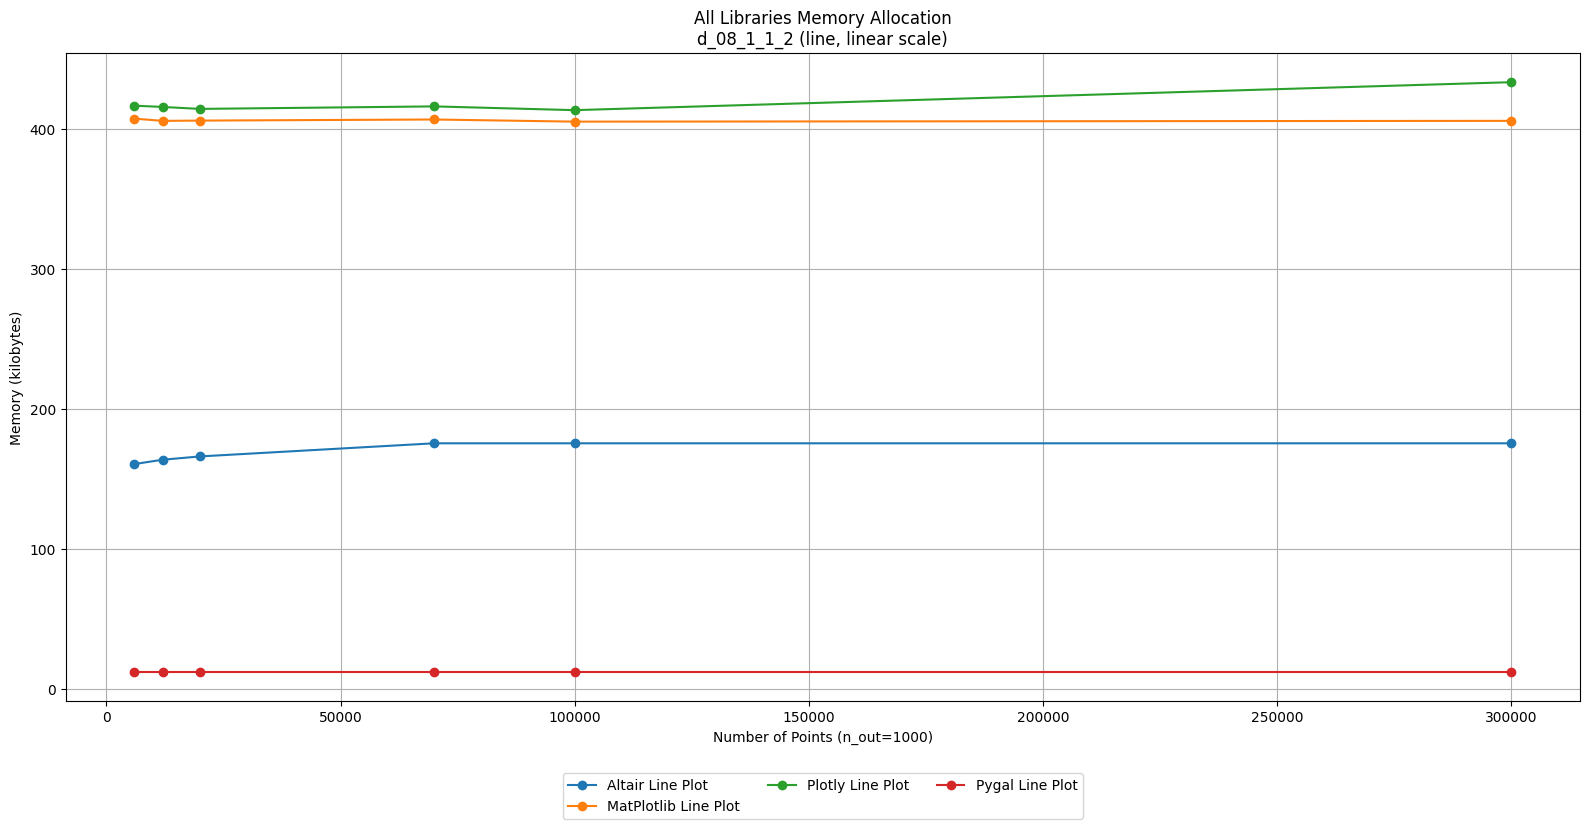
\includegraphics[width=1\textwidth]{anexo/exp/All Libraries Memory Allocation/plots/All Libraries Memory Allocation_d_08_1_1_2_linear_line.png}
        \caption[]{Gráfico de memoria asignada por las diferentes bibliotecas al crear un gráfico para el input \textbf{d\_08\_1\_1\_2}.}
        \label{fig:all_libraries_memory_allocation_plot_line_1}
    \end{figure}
}

\DeclareRobustCommand{\AllLibrariesMemoryAllocationOnePlotBar}{
    %insertar imagen
    \begin{figure}[H]
        \centering
        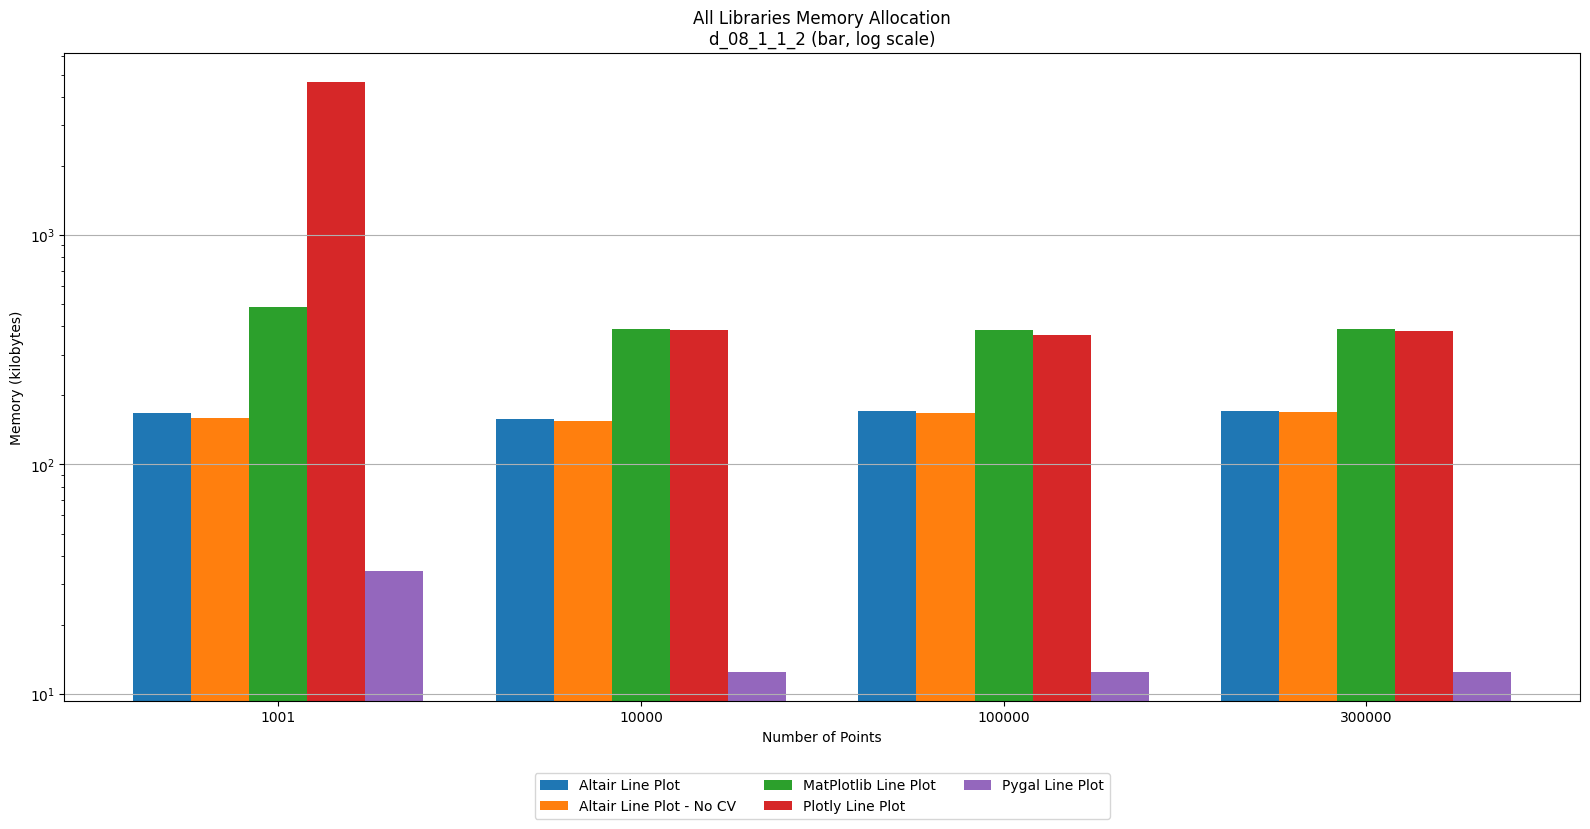
\includegraphics[width=1\textwidth]{anexo/exp/All Libraries Memory Allocation/bar_plots/All Libraries Memory Allocation_d_08_1_1_2_log_bar.png}
        \caption[]{Gráfico de memoria asignada por las diferentes bibliotecas al crear un gráfico para el input \textbf{d\_08\_1\_1\_2}.}
        \label{fig:all_libraries_memory_allocation_plot_bar_1}
    \end{figure}
}

\DeclareRobustCommand{\AllLibrariesMemoryAllocationTwoPlotLine}{
    %insertar imagen
    \begin{figure}[H]
        \centering
        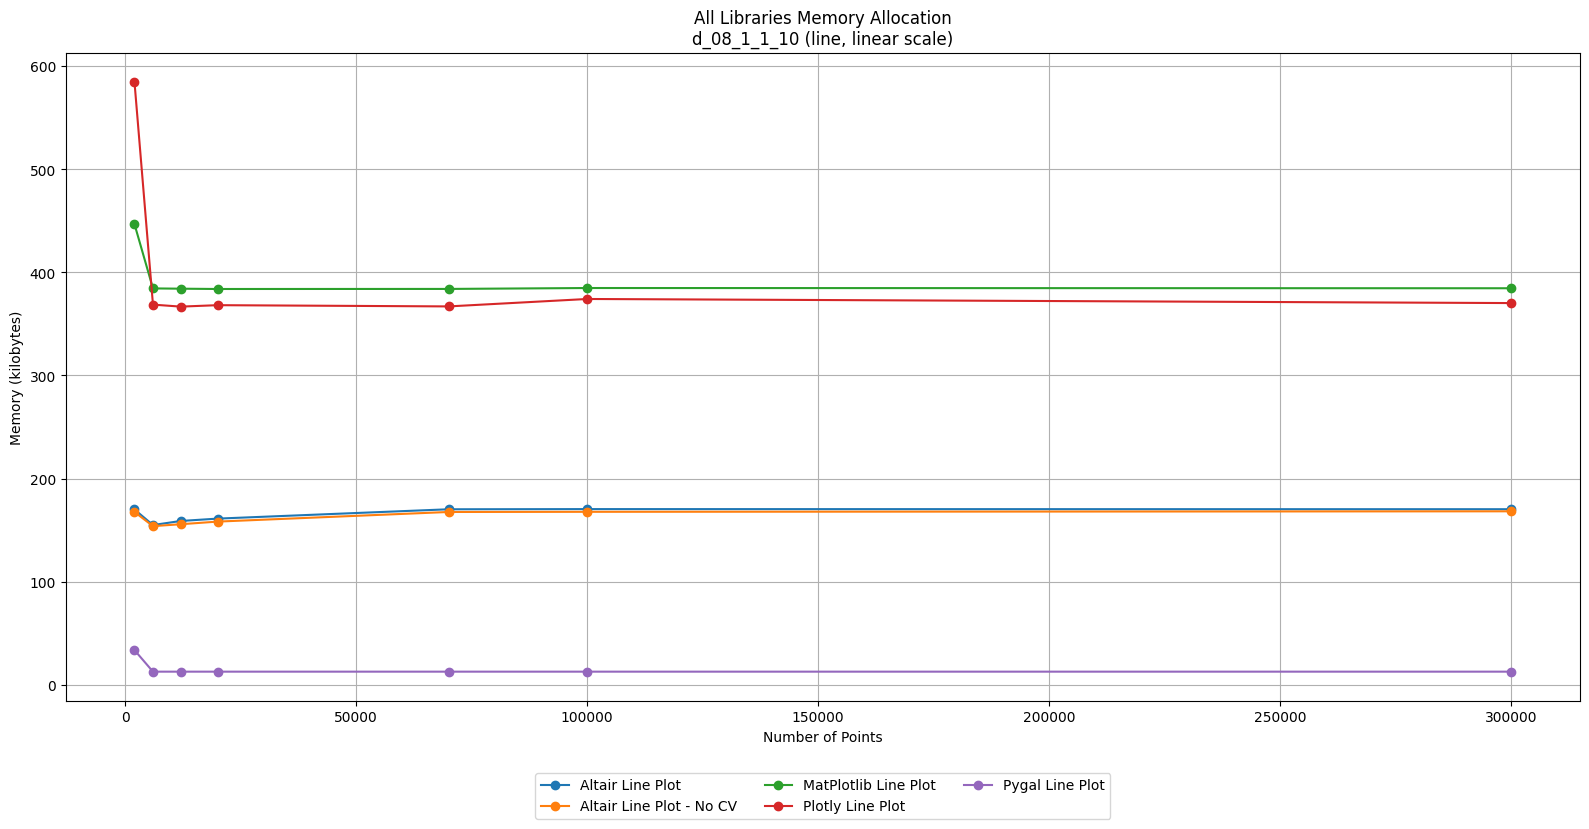
\includegraphics[width=1\textwidth]{anexo/exp/All Libraries Memory Allocation/plots/All Libraries Memory Allocation_d_08_1_1_10_linear_line.png}
        \caption[]{Gráfico de memoria asignada por las diferentes bibliotecas al crear un gráfico para el input \textbf{d\_08\_1\_1\_10}.}
        \label{fig:all_libraries_memory_allocation_plot_line_2}
    \end{figure}
}

\DeclareRobustCommand{\AllLibrariesMemoryAllocationTwoPlotBar}{
    %insertar imagen
    \begin{figure}[H]
        \centering
        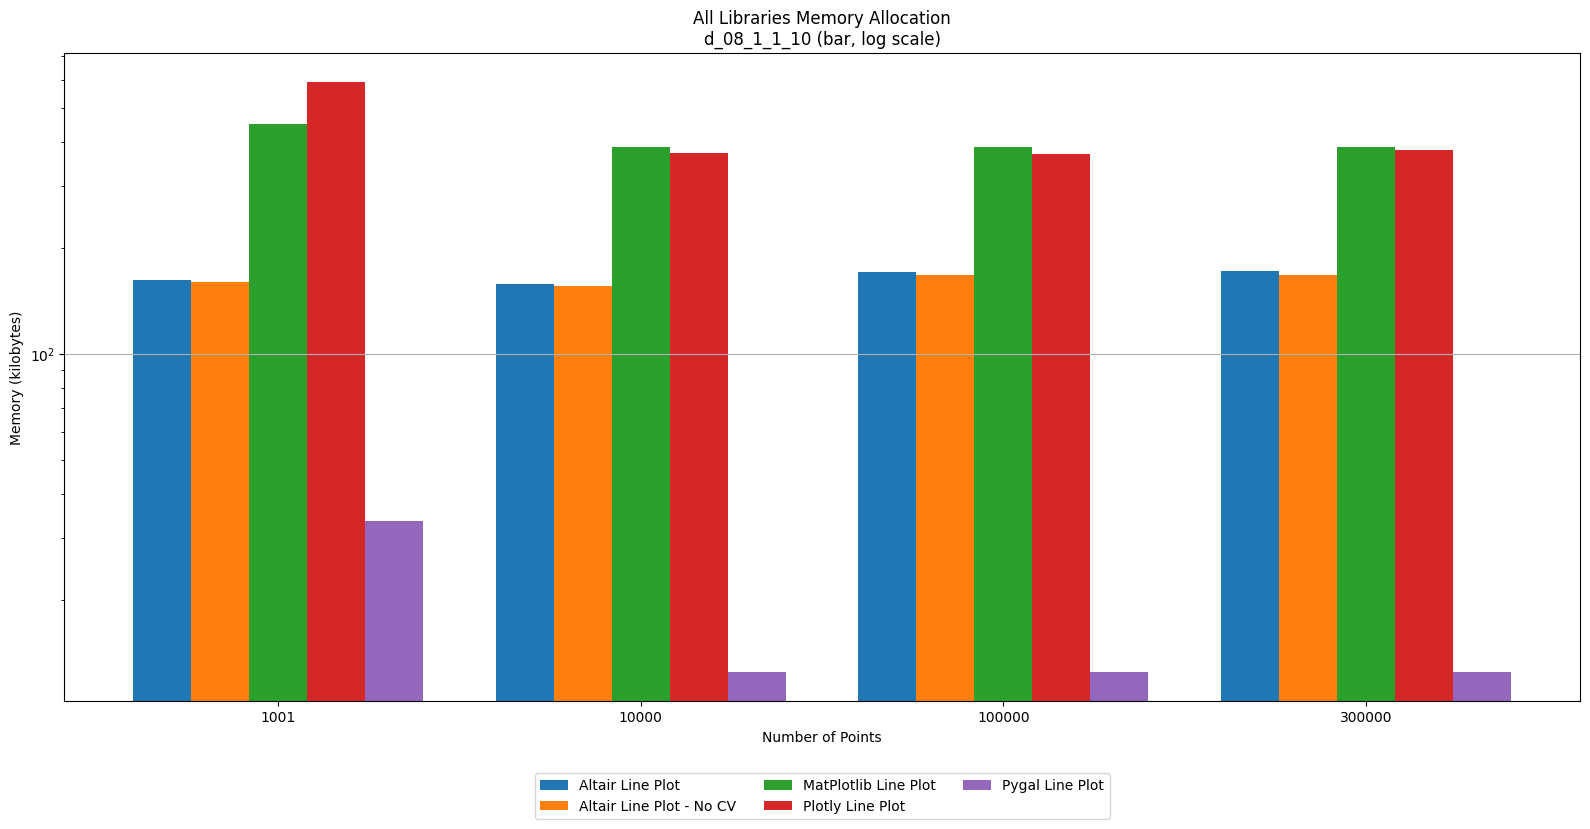
\includegraphics[width=1\textwidth]{anexo/exp/All Libraries Memory Allocation/bar_plots/All Libraries Memory Allocation_d_08_1_1_10_log_bar.png}
        \caption[]{Gráfico de memoria asignada por las diferentes bibliotecas al crear un gráfico para el input \textbf{d\_08\_1\_1\_10}.}
        \label{fig:all_libraries_memory_allocation_plot_bar_2}
    \end{figure}
}

\DeclareRobustCommand{\AllLibrariesMemoryAllocationThreePlotLine}{
    %insertar imagen
    \begin{figure}[H]
        \centering
        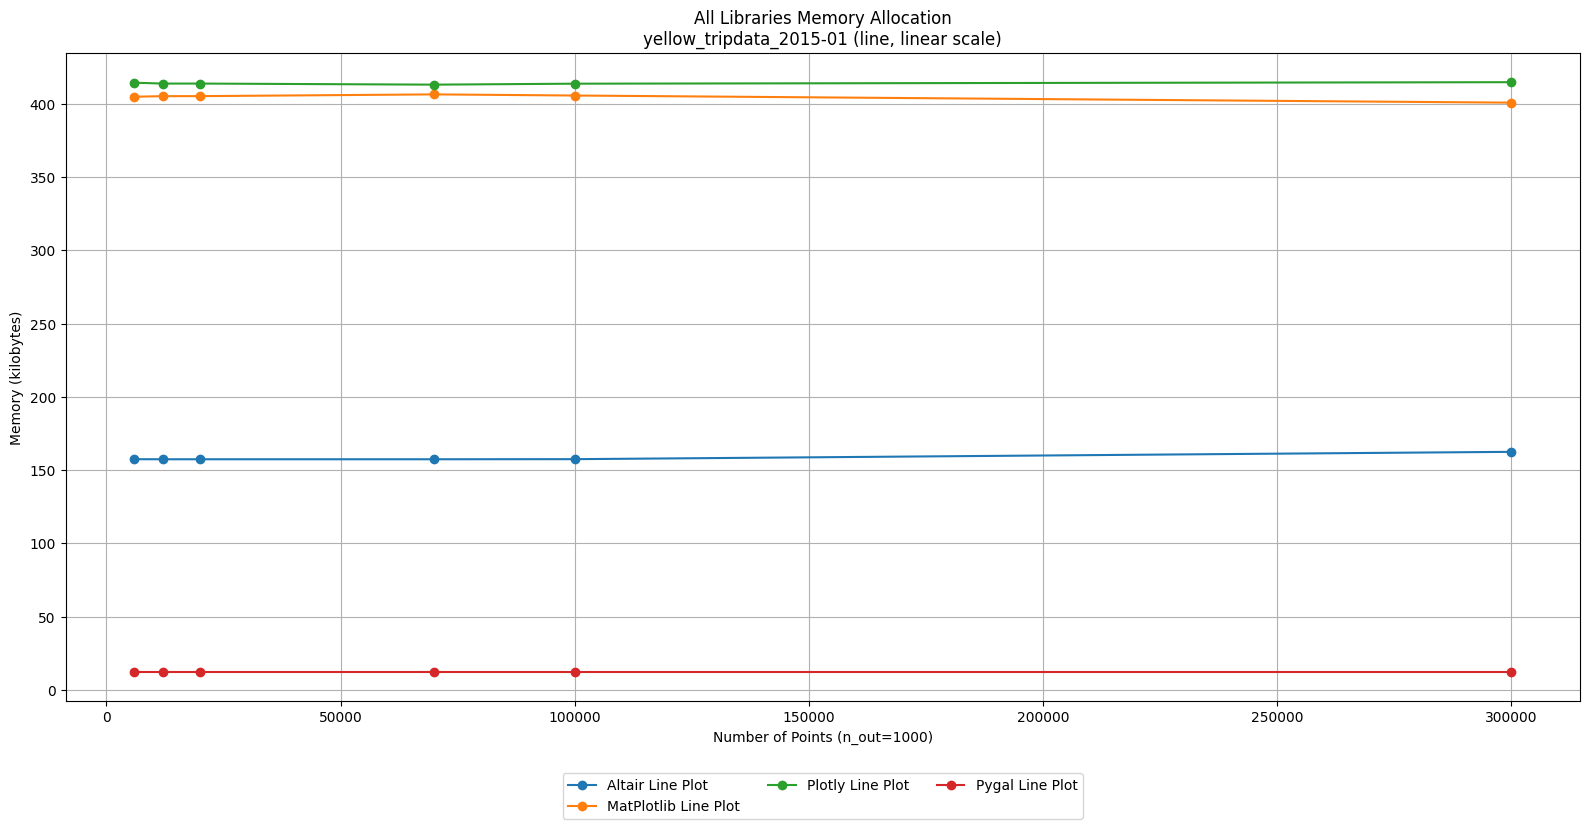
\includegraphics[width=1\textwidth]{anexo/exp/All Libraries Memory Allocation/plots/All Libraries Memory Allocation_yellow_tripdata_2015-01_linear_line.png}
        \caption[]{Gráfico de memoria asignada por las diferentes bibliotecas al crear un gráfico para el input \textbf{yellow\_tripdata\_2015\_01}.}
        \label{fig:all_libraries_memory_allocation_plot_line_3}
    \end{figure}
}

\DeclareRobustCommand{\AllLibrariesMemoryAllocationThreePlotBar}{
    %insertar imagen
    \begin{figure}[H]
        \centering
        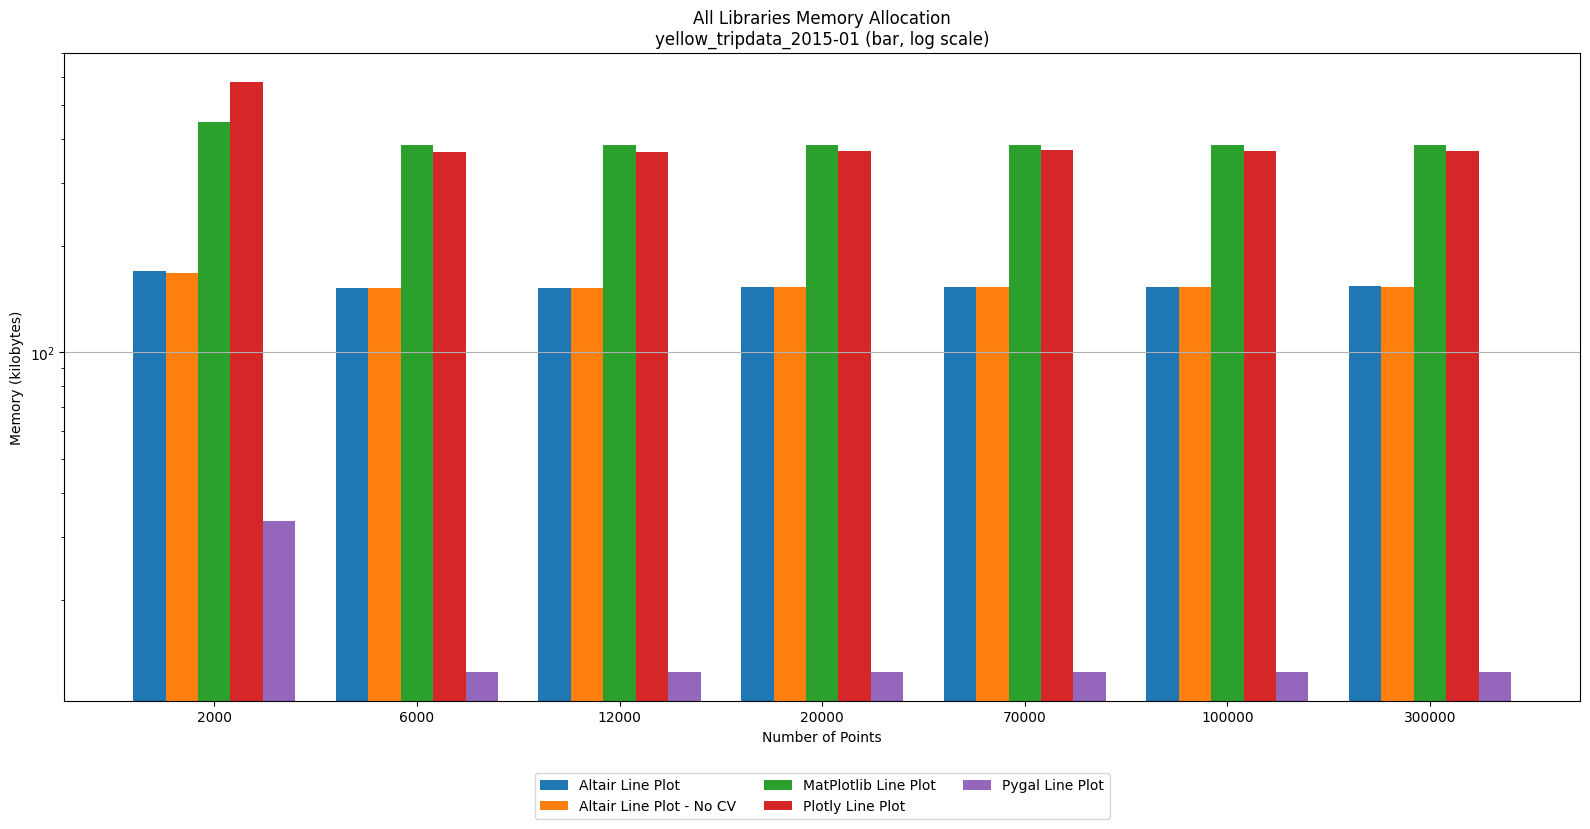
\includegraphics[width=1\textwidth]{anexo/exp/All Libraries Memory Allocation/bar_plots/All Libraries Memory Allocation_yellow_tripdata_2015-01_log_bar.png}
        \caption[]{Gráfico de memoria asignada por las diferentes bibliotecas al crear un gráfico para el input \textbf{yellow\_tripdata\_2015\_01}.}
        \label{fig:all_libraries_memory_allocation_plot_bar_3}
    \end{figure}
}




% All Libraries Time Comparison
\DeclareRobustCommand{\AllLibrariesTimeComparisonOnePlotLine}{
    %insertar imagen
    \begin{figure}[H]
        \centering
        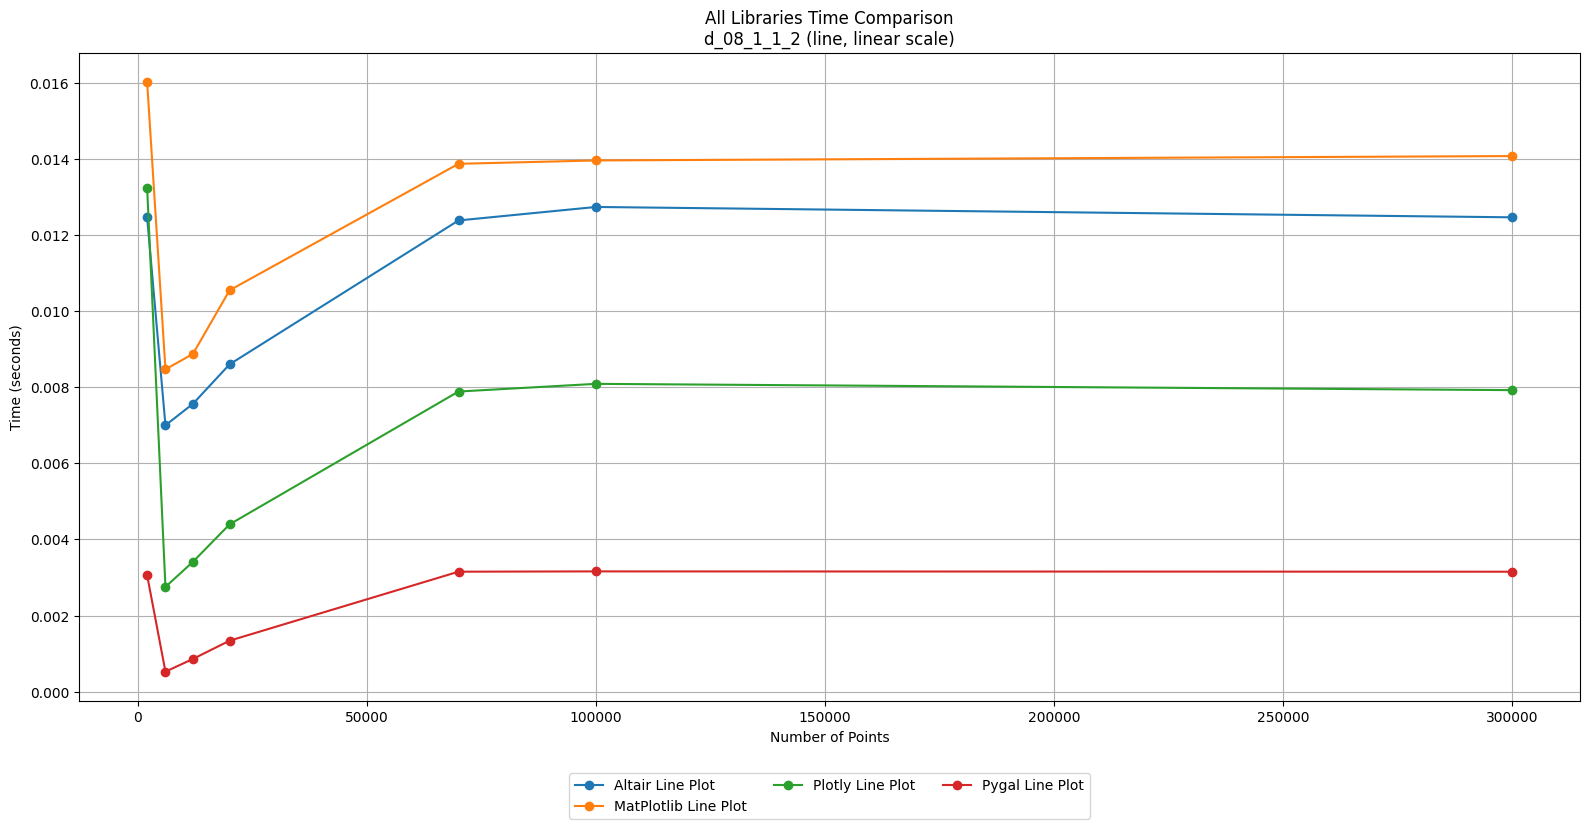
\includegraphics[width=1\textwidth]{anexo/exp/All Libraries Time Comparison/plots/All Libraries Time Comparison_d_08_1_1_2_linear_line.png}
        \caption[]{Gráfico de tiempo de ejecución de las diferentes bibliotecas al crear un gráfico para el input \textbf{d\_08\_1\_1\_2}.}
        \label{fig:all_libraries_time_comparison_plot_line_1}
    \end{figure}
}

\DeclareRobustCommand{\AllLibrariesTimeComparisonOnePlotBar}{
    %insertar imagen
    \begin{figure}[H]
        \centering
        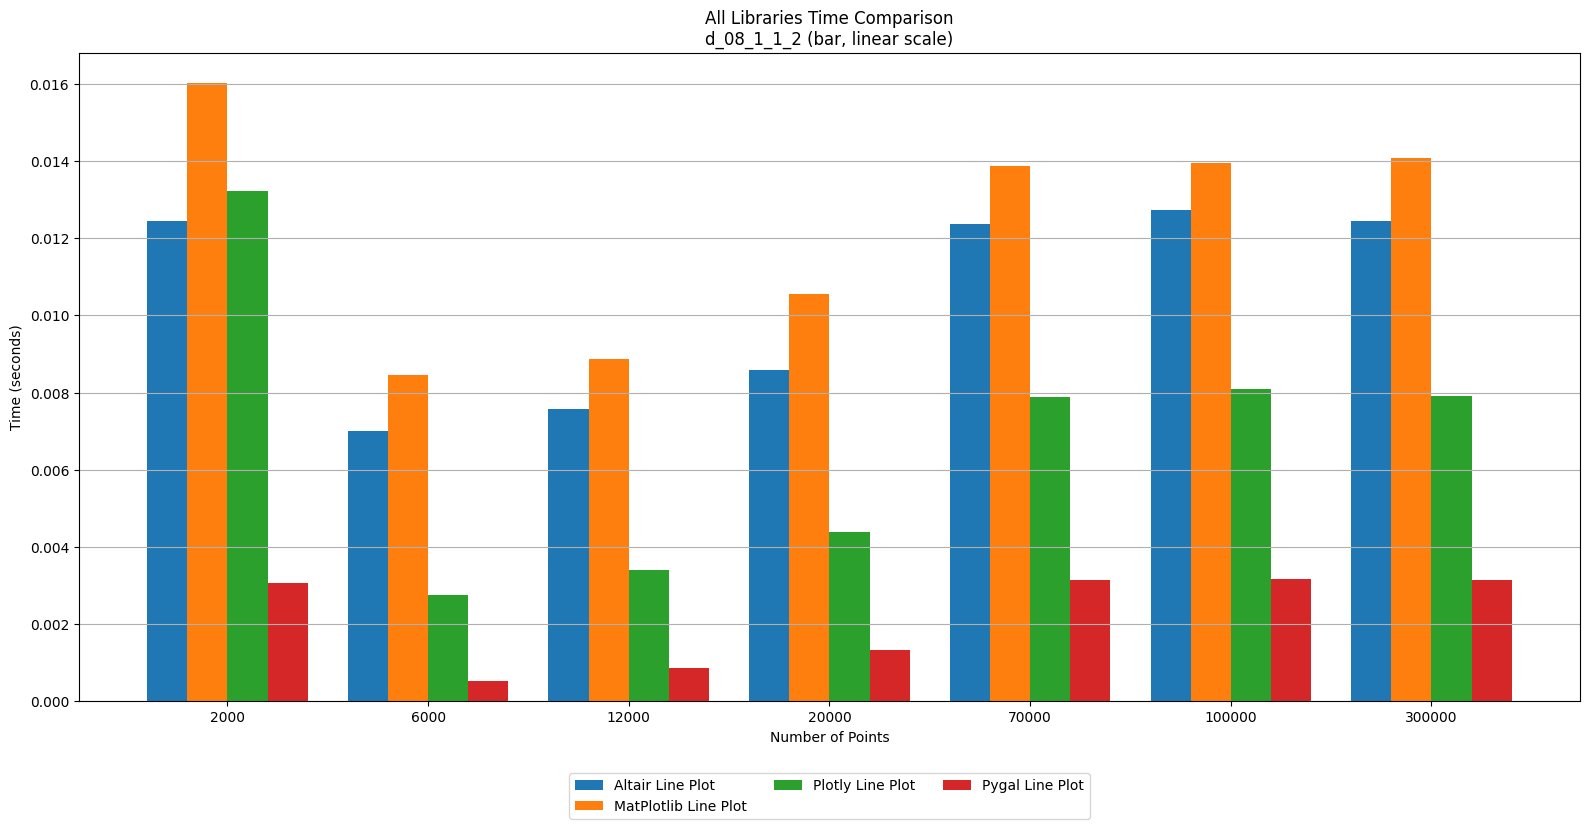
\includegraphics[width=1\textwidth]{anexo/exp/All Libraries Time Comparison/bar_plots/All Libraries Time Comparison_d_08_1_1_2_linear_bar.png}
        \caption[]{Gráfico de tiempo de ejecución de las diferentes bibliotecas al crear un gráfico para el input \textbf{d\_08\_1\_1\_2}.}
        \label{fig:all_libraries_time_comparison_plot_bar_1}
    \end{figure}
}

\DeclareRobustCommand{\AllLibrariesTimeComparisonTwoPlotLine}{
    %insertar imagen
    \begin{figure}[H]
        \centering
        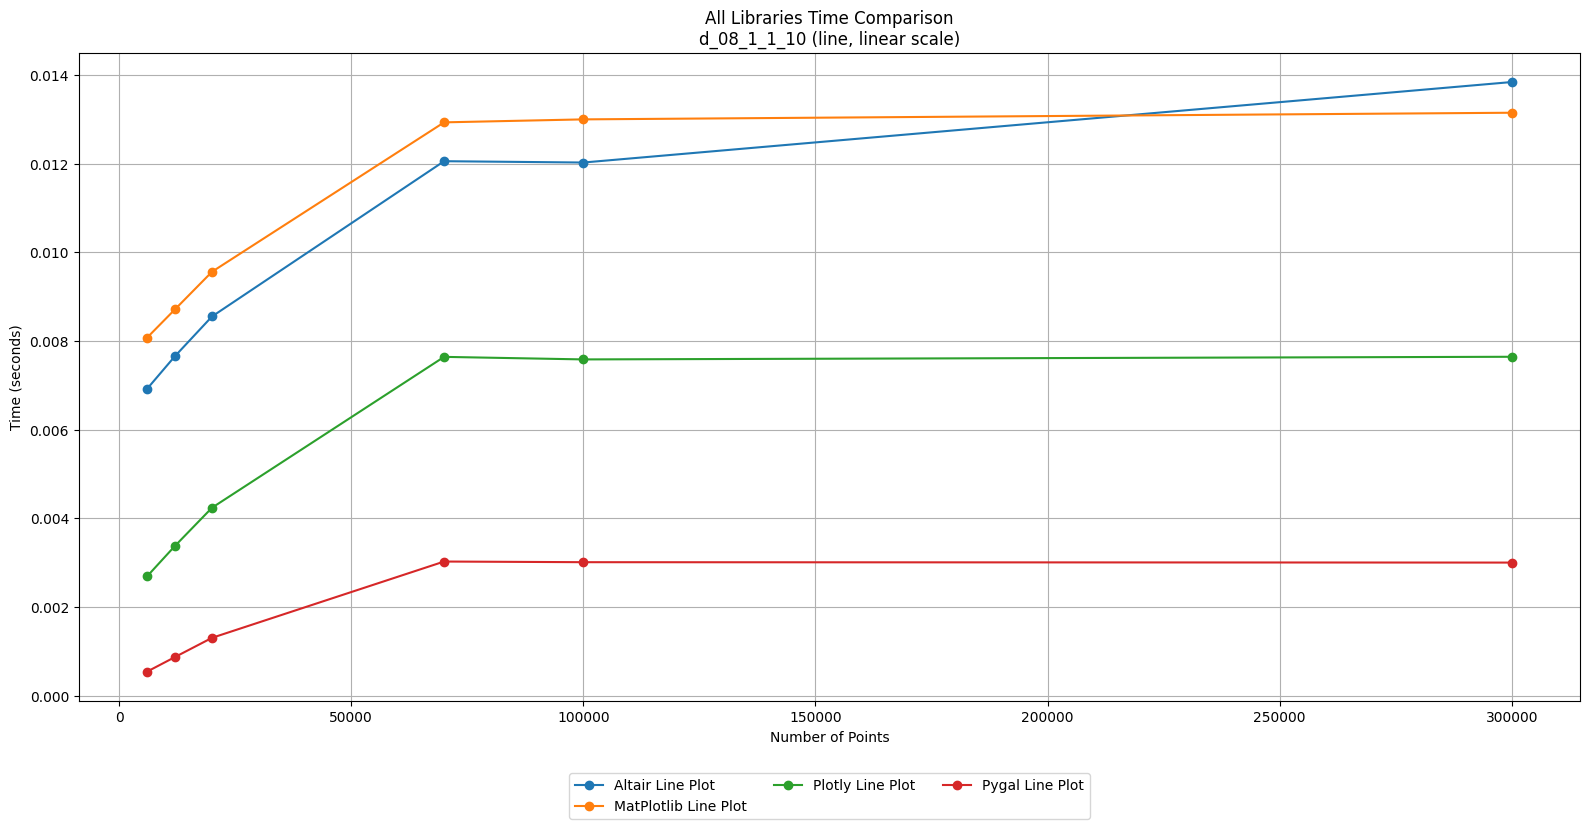
\includegraphics[width=1\textwidth]{anexo/exp/All Libraries Time Comparison/plots/All Libraries Time Comparison_d_08_1_1_10_linear_line.png}
        \caption[]{Gráfico de tiempo de ejecución de las diferentes bibliotecas al crear un gráfico para el input \textbf{d\_08\_1\_1\_10}.}
        \label{fig:all_libraries_time_comparison_plot_line_2}
    \end{figure}
}

\DeclareRobustCommand{\AllLibrariesTimeComparisonTwoPlotBar}{
    %insertar imagen
    \begin{figure}[H]
        \centering
        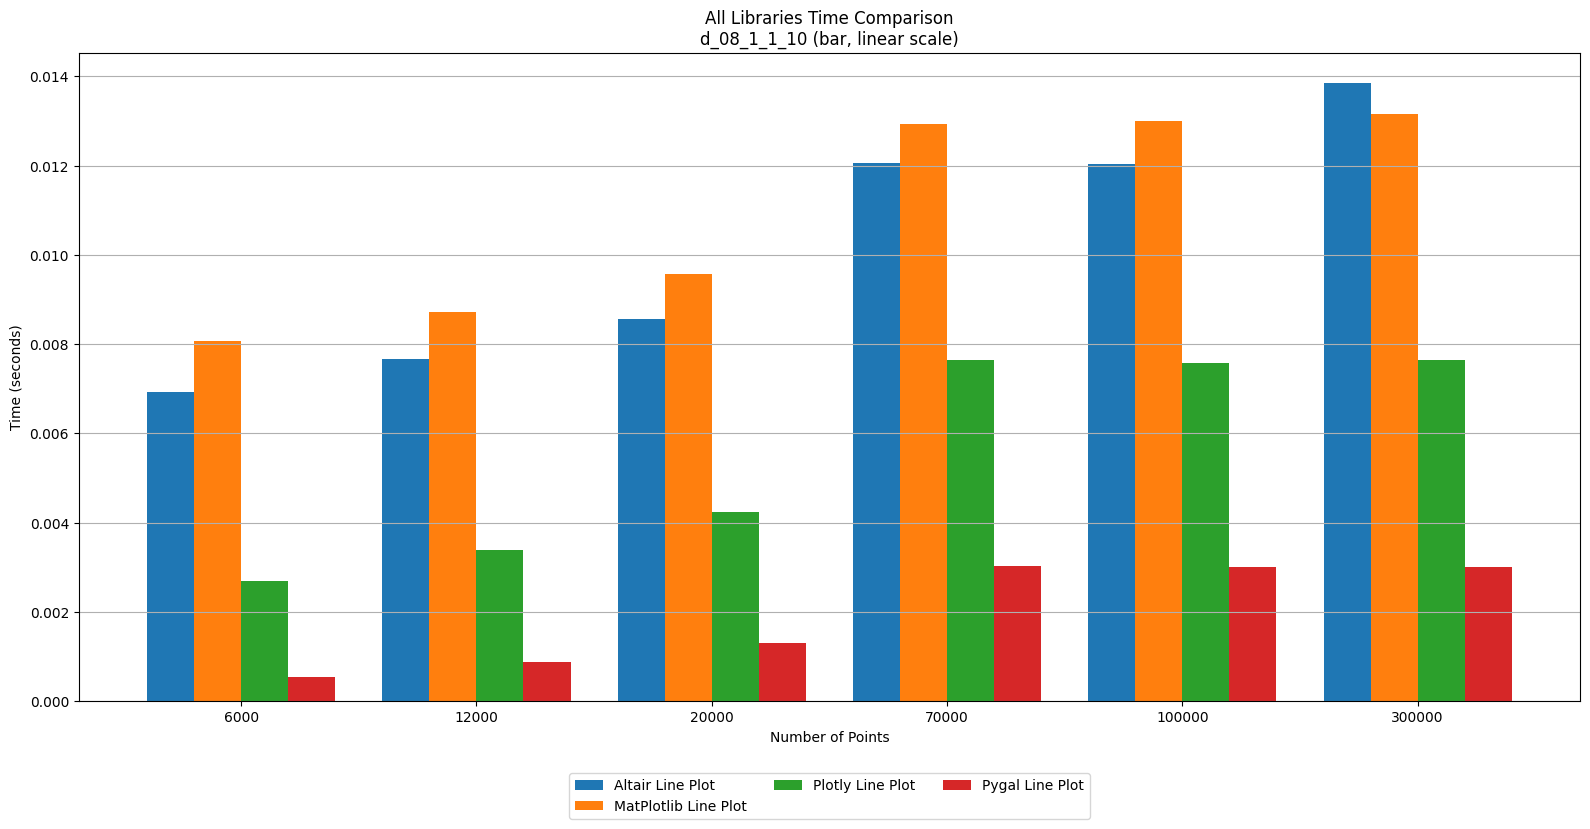
\includegraphics[width=1\textwidth]{anexo/exp/All Libraries Time Comparison/bar_plots/All Libraries Time Comparison_d_08_1_1_10_linear_bar.png}
        \caption[]{Gráfico de tiempo de ejecución de las diferentes bibliotecas al crear un gráfico para el input \textbf{d\_08\_1\_1\_10}.}
        \label{fig:all_libraries_time_comparison_plot_bar_2}
    \end{figure}
}

\DeclareRobustCommand{\AllLibrariesTimeComparisonThreePlotLine}{
    %insertar imagen
    \begin{figure}[H]
        \centering
        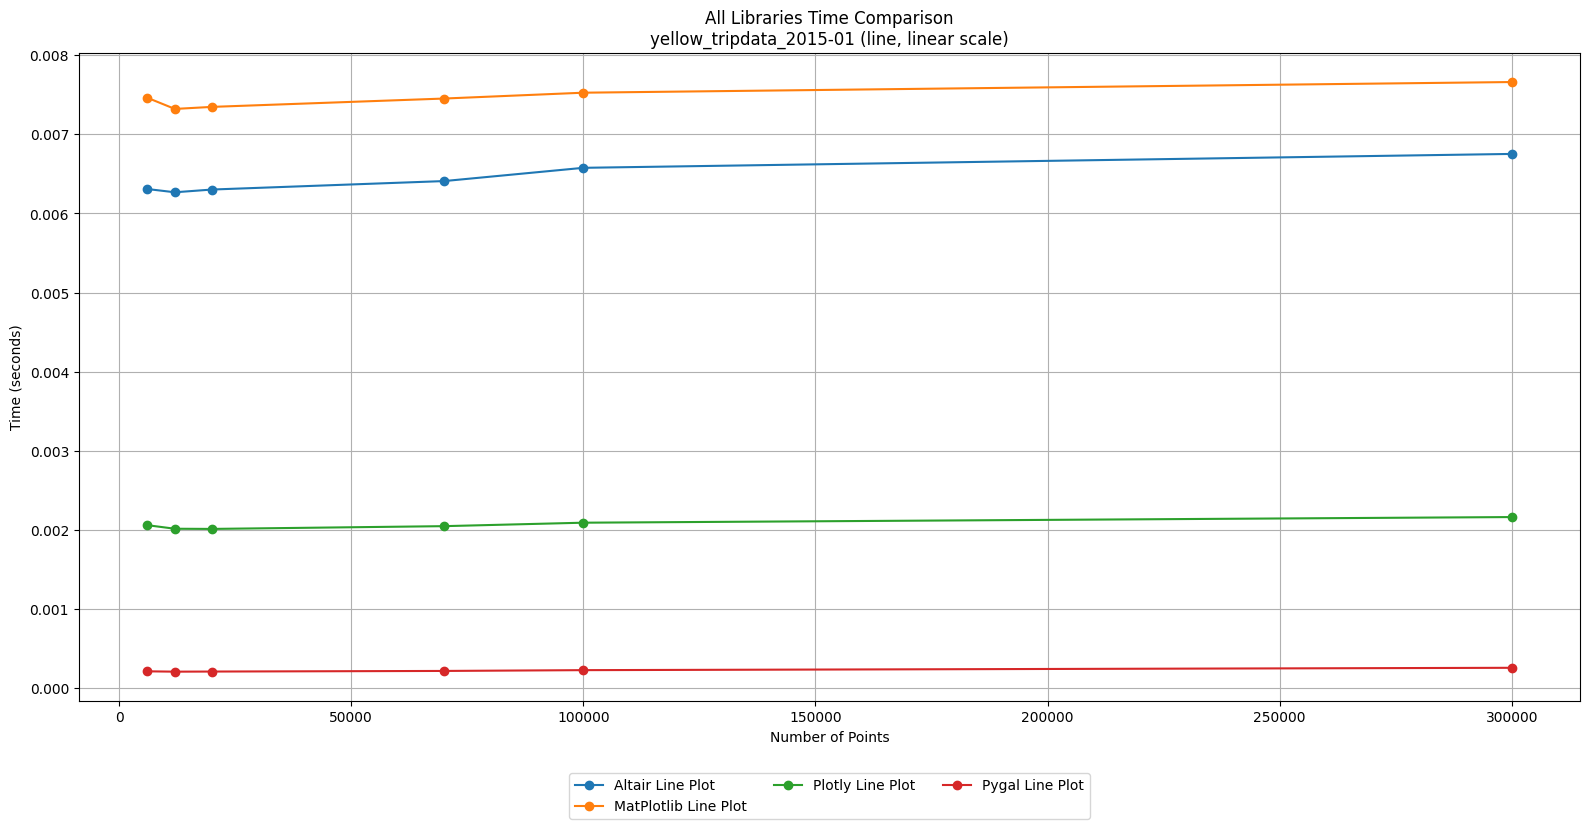
\includegraphics[width=1\textwidth]{anexo/exp/All Libraries Time Comparison/plots/All Libraries Time Comparison_yellow_tripdata_2015-01_linear_line.png}
        \caption[]{Gráfico de tiempo de ejecución de las diferentes bibliotecas al crear un gráfico para el input \textbf{yellow\_tripdata\_2015\_01}.}
        \label{fig:all_libraries_time_comparison_plot_line_3}
    \end{figure}
}

\DeclareRobustCommand{\AllLibrariesTimeComparisonThreePlotBar}{
    %insertar imagen
    \begin{figure}[H]
        \centering
        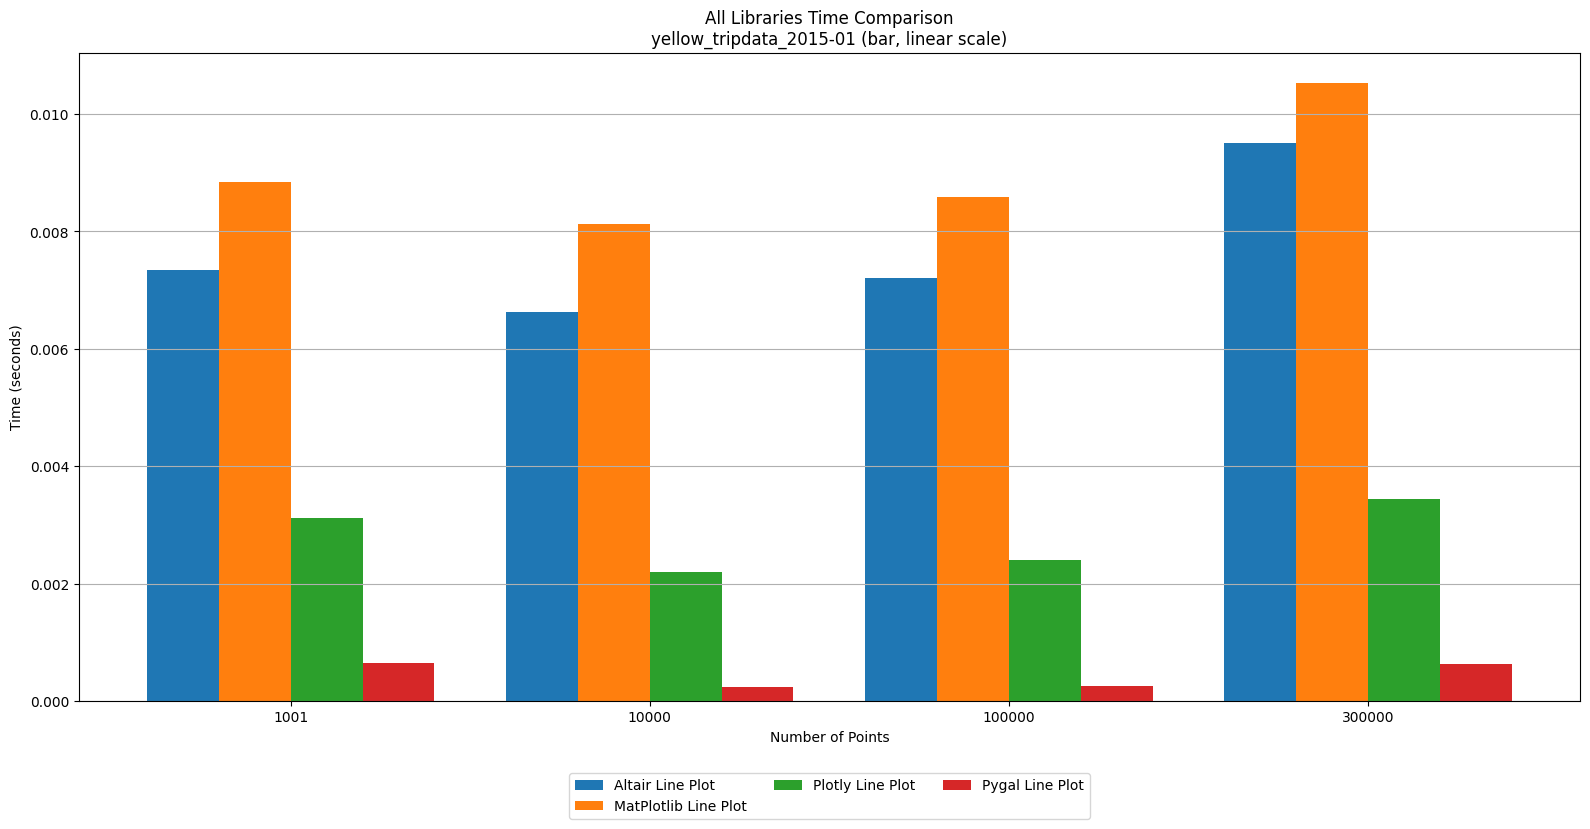
\includegraphics[width=1\textwidth]{anexo/exp/All Libraries Time Comparison/bar_plots/All Libraries Time Comparison_yellow_tripdata_2015-01_linear_bar.png}
        \caption[]{Gráfico de tiempo de ejecución de las diferentes bibliotecas al crear un gráfico para el input \textbf{yellow\_tripdata\_2015\_01}.}
        \label{fig:all_libraries_time_comparison_plot_bar_3}
    \end{figure}
}

Building Time Comparison
\DeclareRobustCommand{\BuildingTimeComparisonOnePlotLine}{
    %insertar imagen
    \begin{figure}[H]
        \centering
        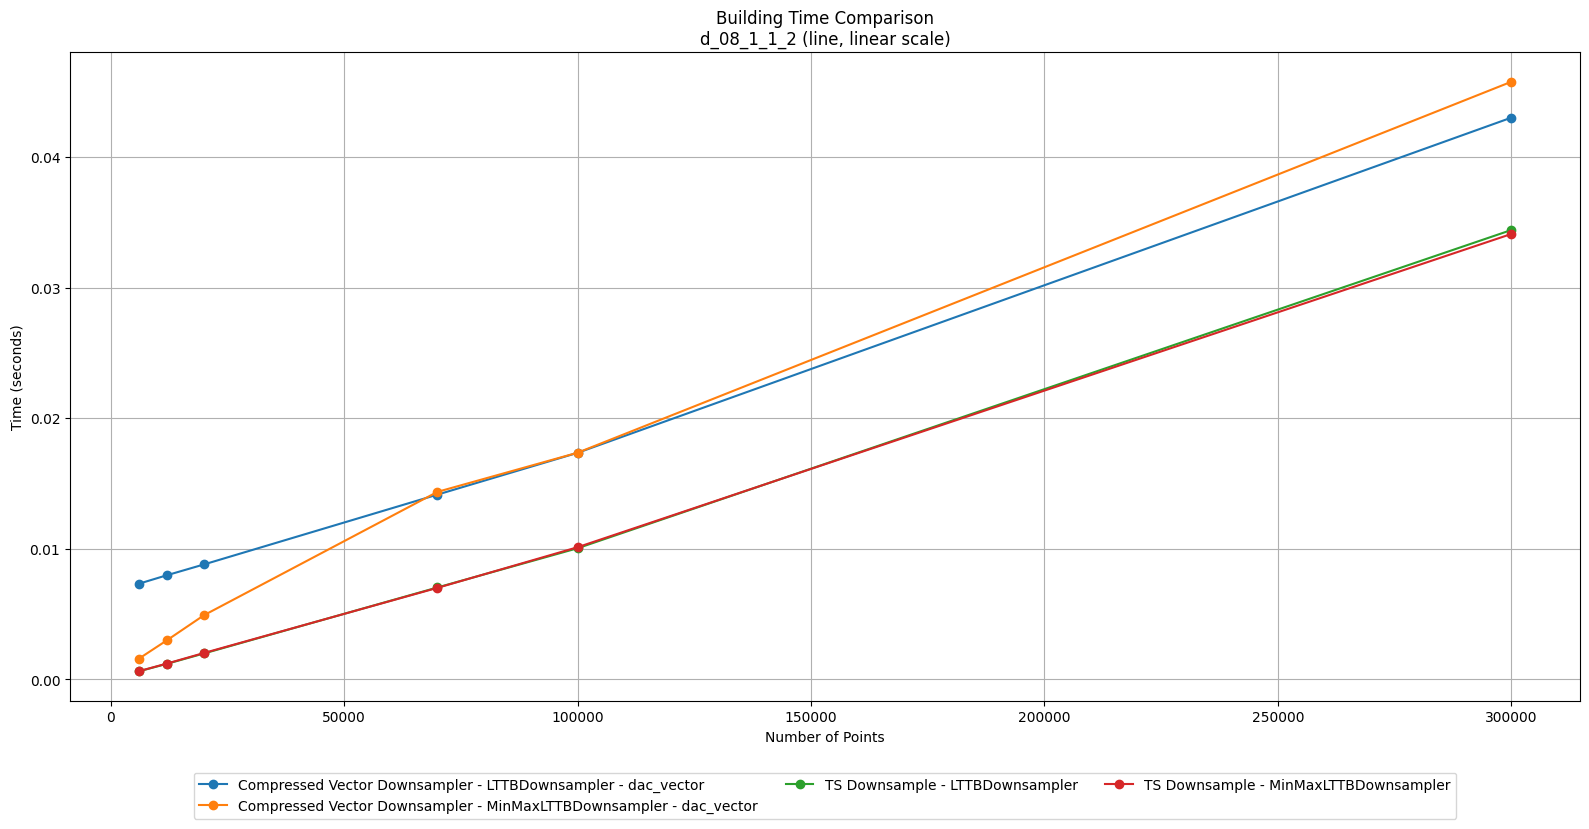
\includegraphics[width=1\textwidth]{anexo/exp/Building Time Comparison/plots/Building Time Comparison_d_08_1_1_2_linear_line.png}
        \caption[]{Gráfico de tiempo de construcción de las diferentes bibliotecas para el input \textbf{d\_08\_1\_1\_2}.}
        \label{fig:building_time_comparison_plot_line_1}
    \end{figure}
}

\DeclareRobustCommand{\BuildingTimeComparisonOnePlotBar}{
    %insertar imagen
    \begin{figure}[H]
        \centering
        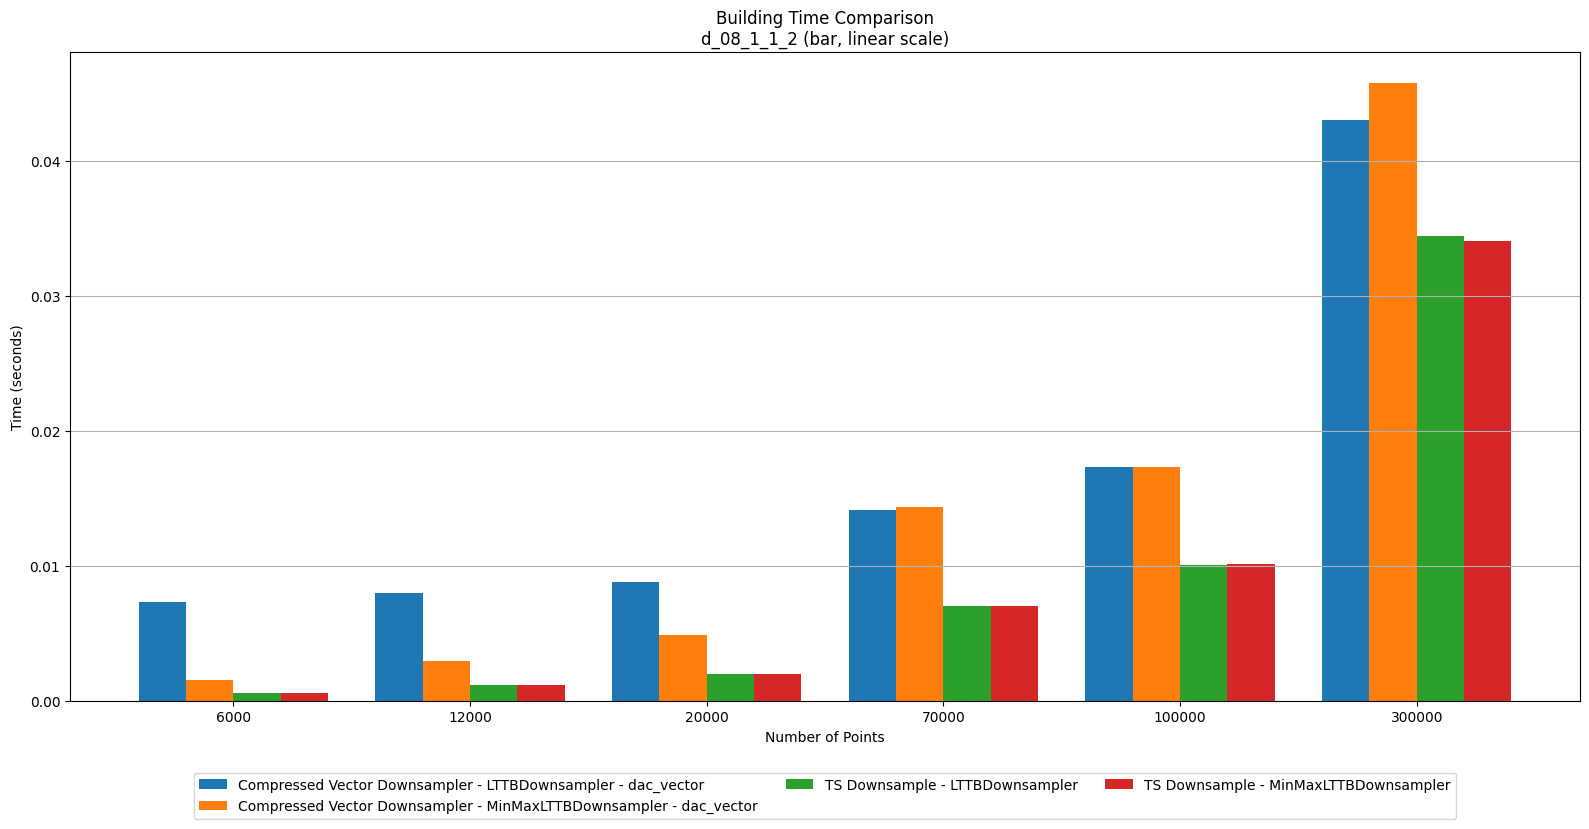
\includegraphics[width=1\textwidth]{anexo/exp/Building Time Comparison/bar_plots/Building Time Comparison_d_08_1_1_2_linear_bar.png}
        \caption[]{Gráfico de tiempo de construcción de las diferentes bibliotecas para el input \textbf{d\_08\_1\_1\_2}.}
        \label{fig:building_time_comparison_plot_bar_1}
    \end{figure}
}

\DeclareRobustCommand{\BuildingTimeComparisonTwoPlotLine}{
    %insertar imagen
    \begin{figure}[H]
        \centering
        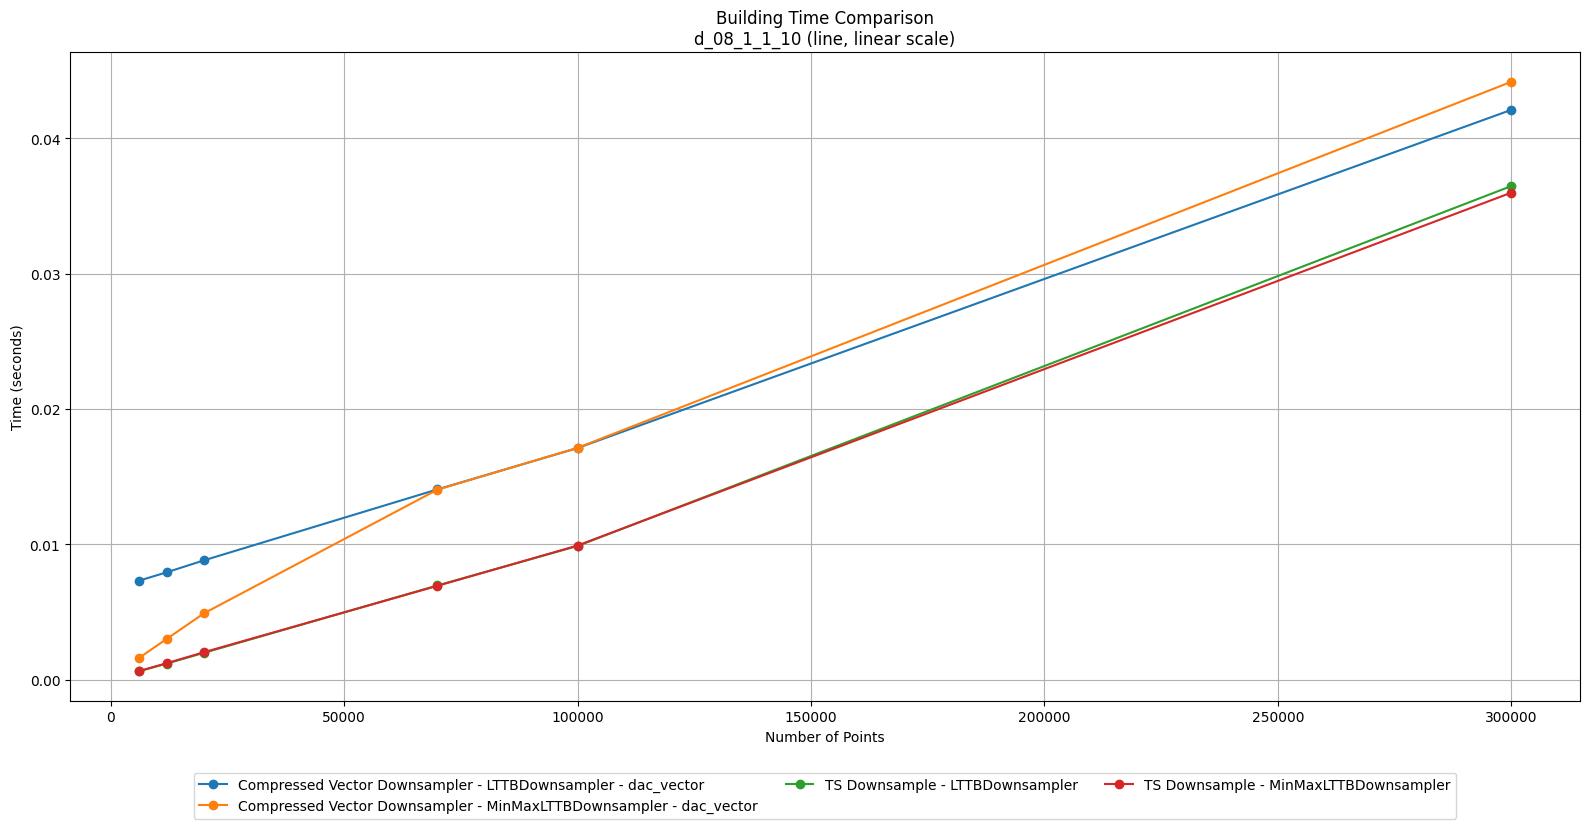
\includegraphics[width=1\textwidth]{anexo/exp/Building Time Comparison/plots/Building Time Comparison_d_08_1_1_10_linear_line.png}
        \caption[]{Gráfico de tiempo de construcción de las diferentes bibliotecas para el input \textbf{d\_08\_1\_1\_10}.}
        \label{fig:building_time_comparison_plot_line_2}
    \end{figure}
}

\DeclareRobustCommand{\BuildingTimeComparisonTwoPlotBar}{
    %insertar imagen
    \begin{figure}[H]
        \centering
        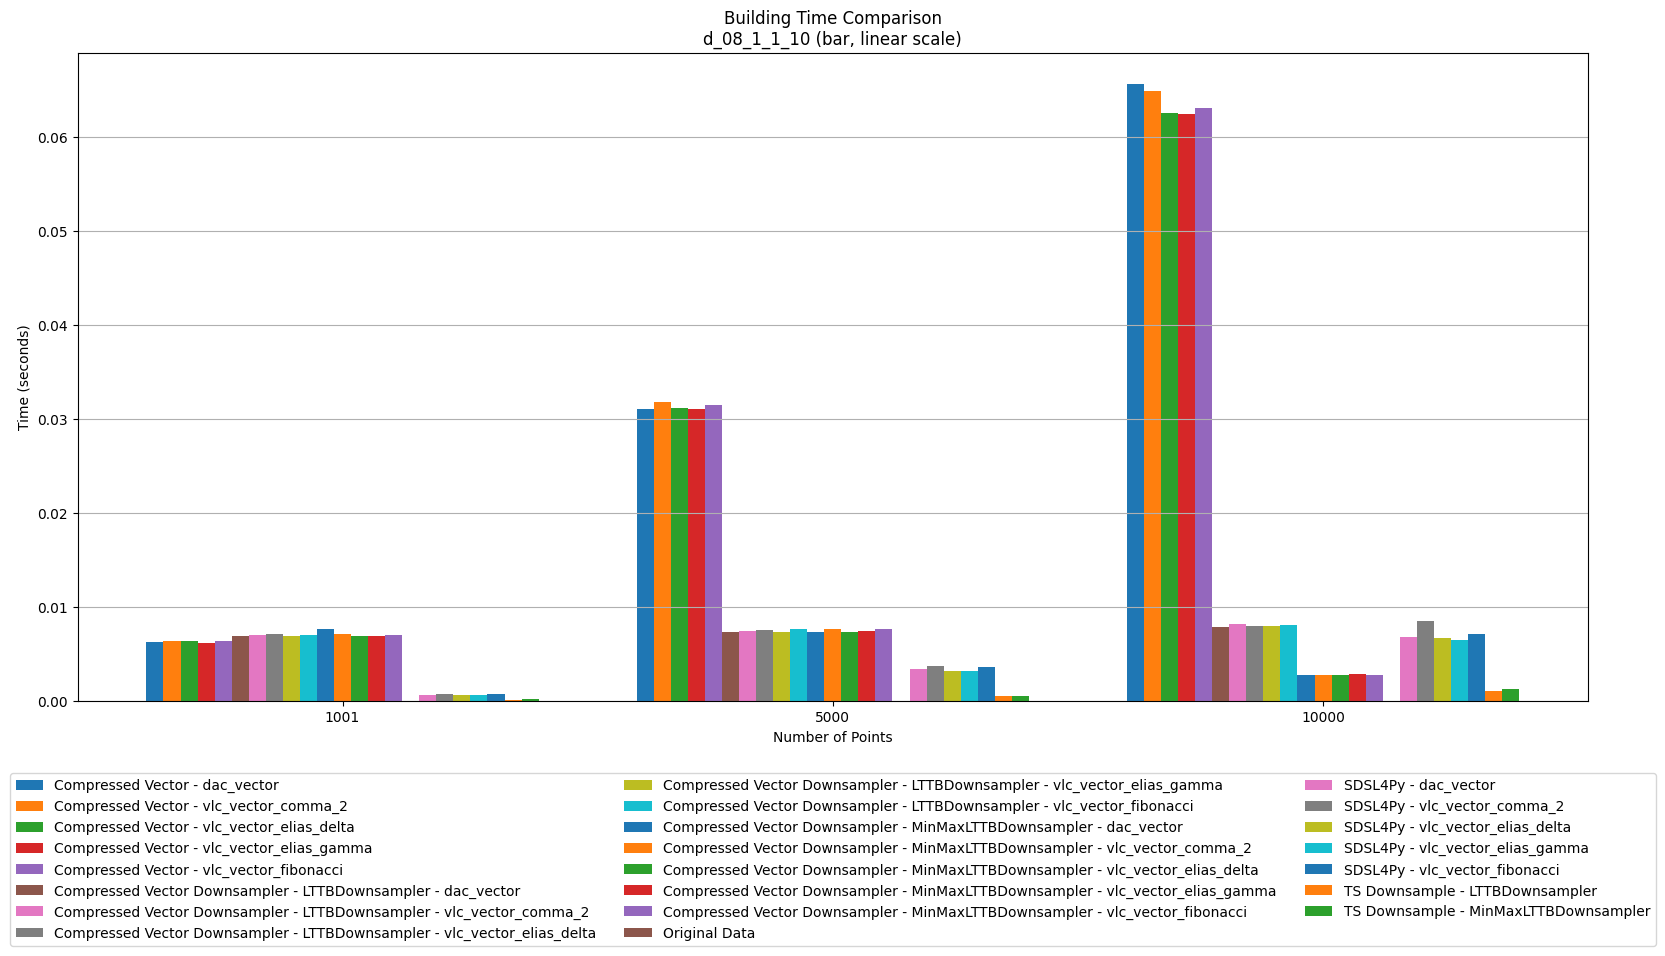
\includegraphics[width=1\textwidth]{anexo/exp/Building Time Comparison/bar_plots/Building Time Comparison_d_08_1_1_10_linear_bar.png}
        \caption[]{Gráfico de tiempo de construcción de las diferentes bibliotecas para el input \textbf{d\_08\_1\_1\_10}.}
        \label{fig:building_time_comparison_plot_bar_2}
    \end{figure}
}

\DeclareRobustCommand{\BuildingTimeComparisonThreePlotLine}{
    %insertar imagen
    \begin{figure}[H]
        \centering
        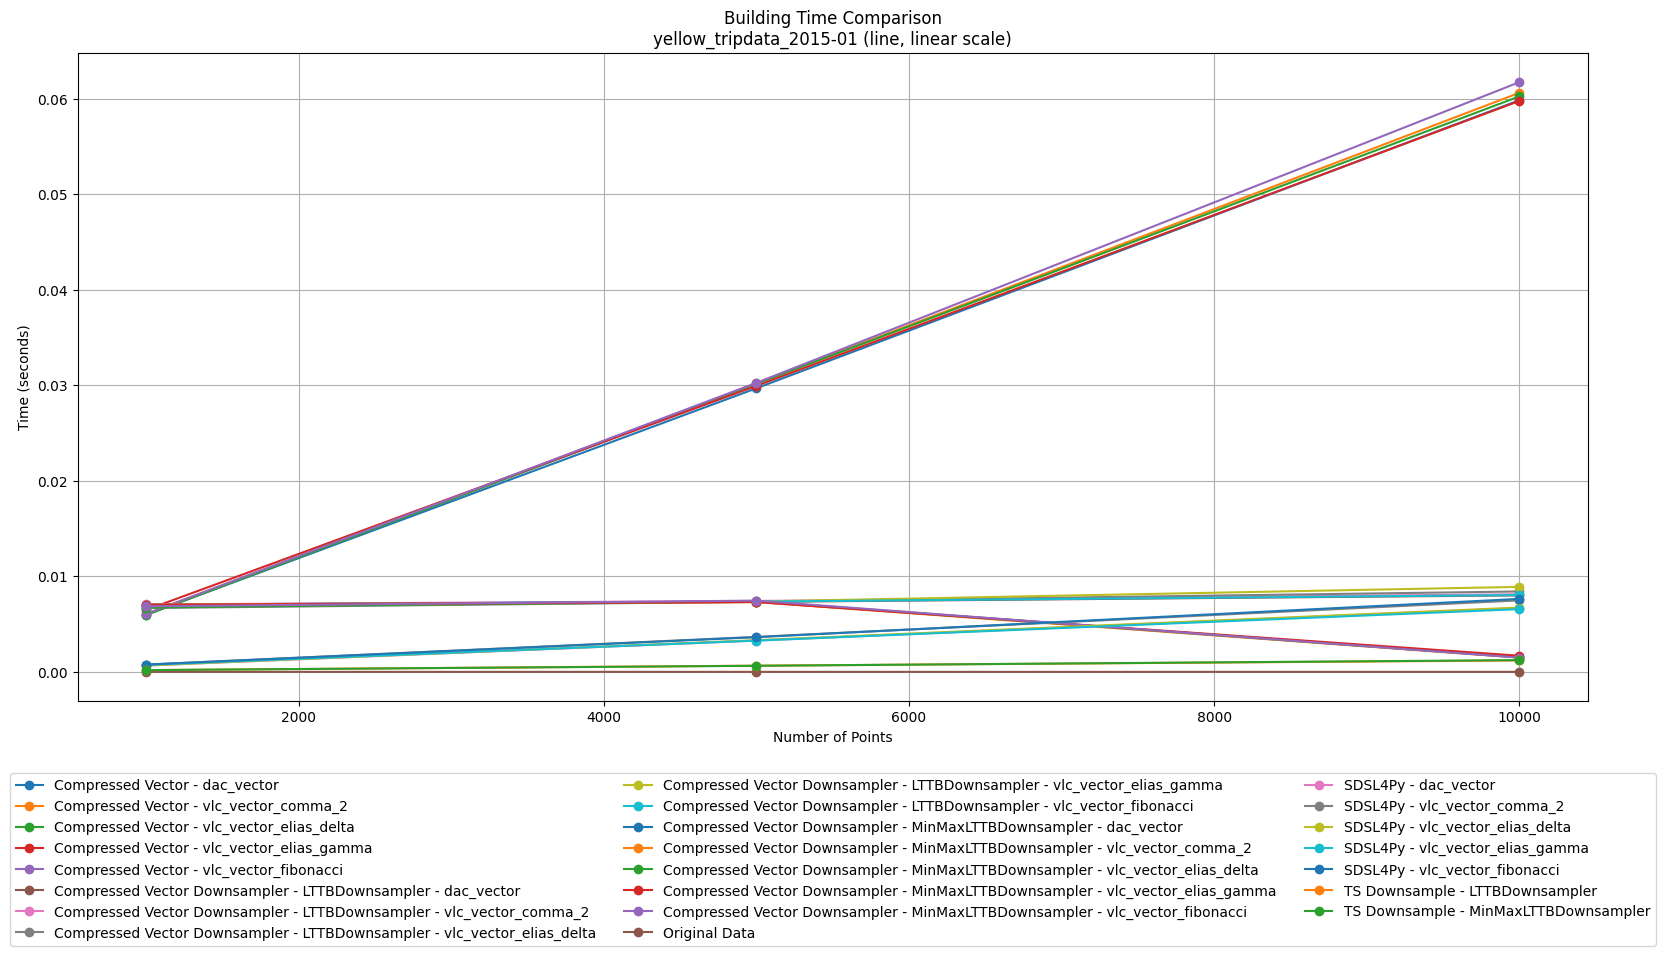
\includegraphics[width=1\textwidth]{anexo/exp/Building Time Comparison/plots/Building Time Comparison_yellow_tripdata_2015-01_linear_line.png}
        \caption[]{Gráfico de tiempo de construcción de las diferentes bibliotecas para el input \textbf{yellow\_tripdata\_2015\_01}.}
        \label{fig:building_time_comparison_plot_line_3}
    \end{figure}
}

\DeclareRobustCommand{\BuildingTimeComparisonThreePlotBar}{
    %insertar imagen
    \begin{figure}[H]
        \centering
        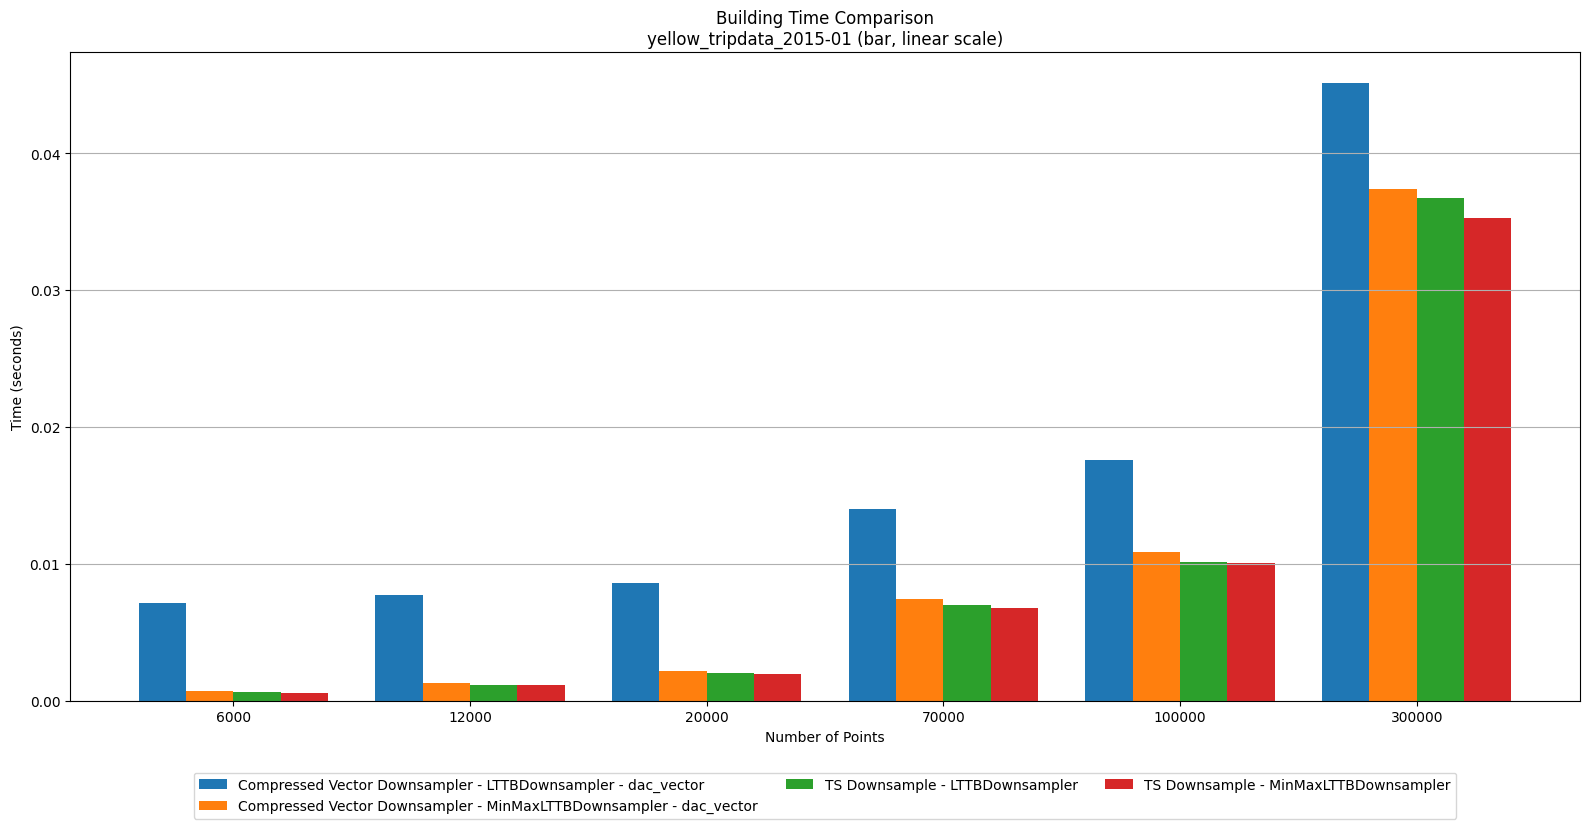
\includegraphics[width=1\textwidth]{anexo/exp/Building Time Comparison/bar_plots/Building Time Comparison_yellow_tripdata_2015-01_linear_bar.png}
        \caption[]{Gráfico de tiempo de construcción de las diferentes bibliotecas para el input \textbf{yellow\_tripdata\_2015\_01}.}
        \label{fig:building_time_comparison_plot_bar_3}
    \end{figure}
}




% Comparison of Space Used
\DeclareRobustCommand{\ComparisonOfSpaceUsedOnePlotLine}{
    %insertar imagen
    \begin{figure}[H]
        \centering
        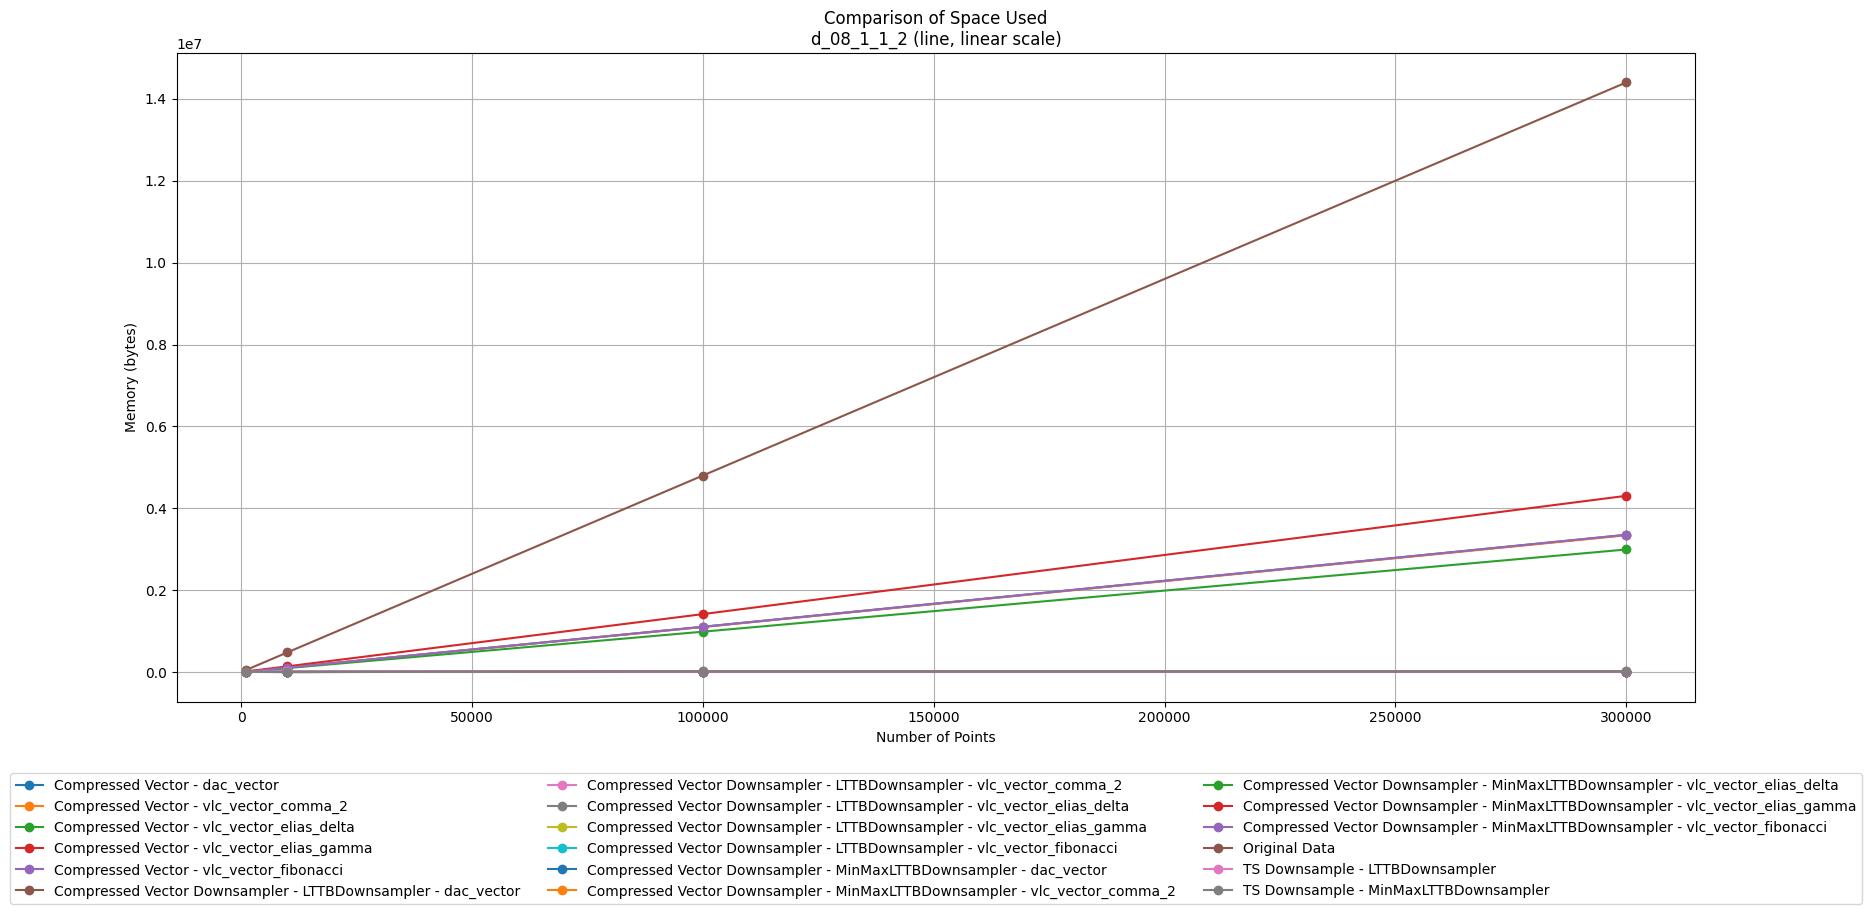
\includegraphics[width=1\textwidth]{anexo/exp/Comparison of Space Used/plots/Comparison of Space Used_d_08_1_1_2_linear_line.png}
        \caption[]{Gráfico de espacio usado por las diferentes bibliotecas para el input \textbf{d\_08\_1\_1\_2}.}
        \label{fig:comparison_of_space_used_plot_line_1}
    \end{figure}
}

\DeclareRobustCommand{\ComparisonOfSpaceUsedOnePlotBar}{
    %insertar imagen
    \begin{figure}[H]
        \centering
        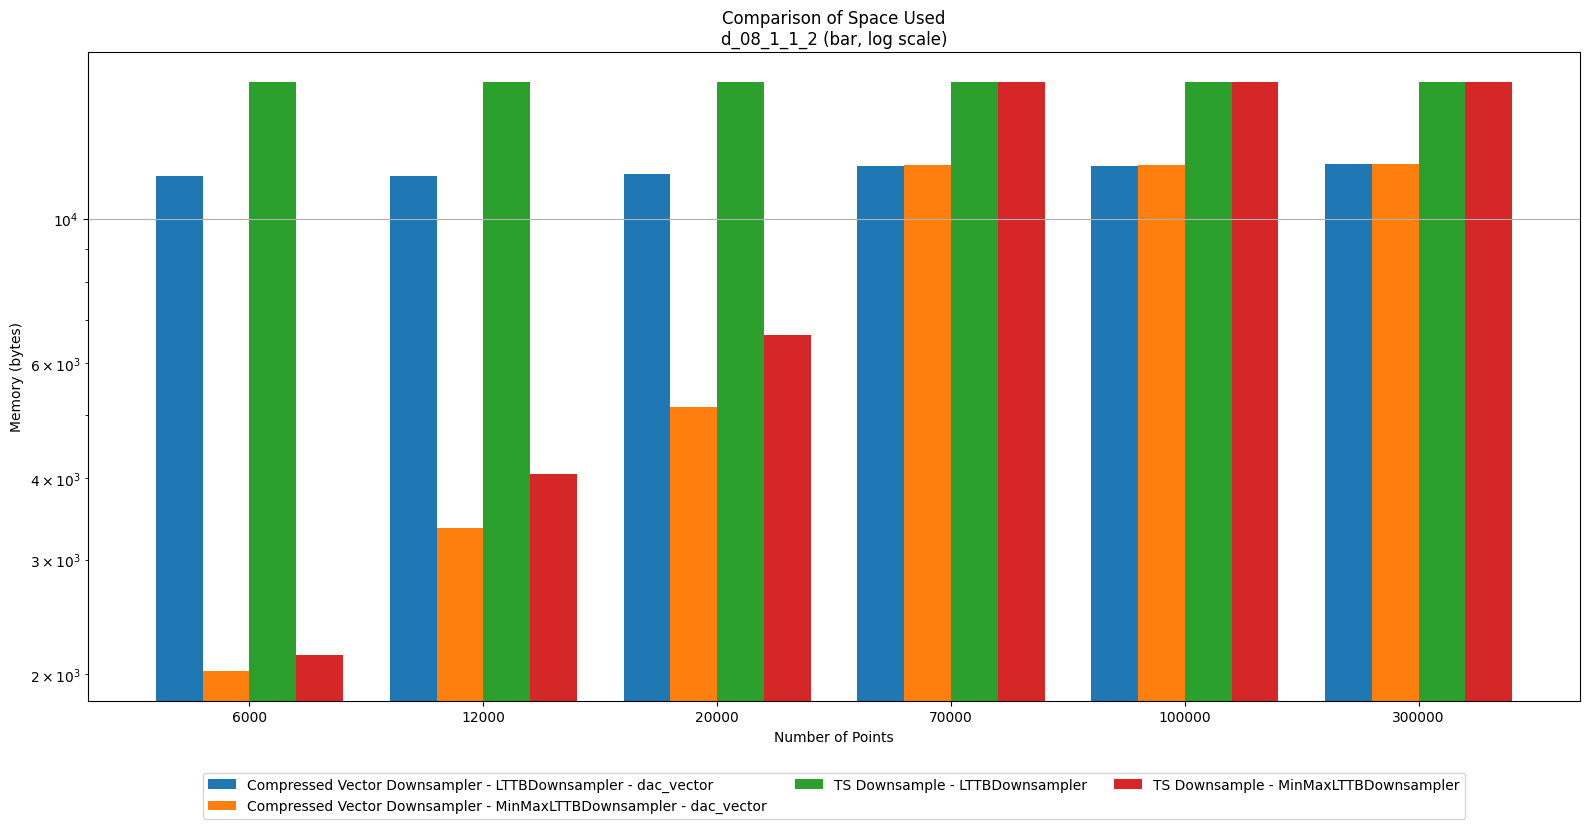
\includegraphics[width=1\textwidth]{anexo/exp/Comparison of Space Used/bar_plots/Comparison of Space Used_d_08_1_1_2_log_bar.png}
        \caption[]{Gráfico de espacio usado por las diferentes bibliotecas para el input \textbf{d\_08\_1\_1\_2}.}
        \label{fig:comparison_of_space_used_plot_bar_1}
    \end{figure}
    \begin{table}[H]
        \centering
        \resizebox{\textwidth}{!}{%
        \begin{tabular}{|l|c|c|c|c|c|c|}
        \hline\multicolumn{1}{|c|}{Option} & \multicolumn{6}{c|}{\textbf{Number of data points}} \\
        \cline{2-7}
         & \textbf{6000} & \textbf{12000} & \textbf{20000} & \textbf{70000} & \textbf{100000} & \textbf{300000} \\
        \hline
        Compressed Vector Downsample - dac\_vector & 1.66e+03 [B] & 2.68e+03 [B] & 4.07e+03 [B] & 9.49e+03 [B] & 9.48e+03 [B] & 9.54e+03 [B] \\
        Compressed Vector Downsample - vlc\_vector\_fibonacci & 1.24e+03 [B] & 2.26e+03 [B] & 3.65e+03 [B] & 8.89e+03 [B] & 8.88e+03 [B] & 9.04e+03 [B] \\
        Original Data & 1.06e+05 [B] & 2.16e+05 [B] & 3.46e+05 [B] & 1.12e+06 [B] & 1.60e+06 [B] & 5.20e+06 [B] \\
        TS Downsample & 2.14e+03 [B] & 4.06e+03 [B] & 6.62e+03 [B] & 1.62e+04 [B] & 1.62e+04 [B] & 1.62e+04 [B] \\
        \hline
        \end{tabular}
        }
        \label{tab:comparison of space used-d-08-1-1-2}
    \end{table}
    \begin{table}[H]
        \centering
        \caption{Comparison of Space Used\_d\_08\_1\_1\_2 – Tasa de compactación CVD vs TS vs Datos Originales}
        \label{tab:Comparison of Space Used\_d\_08\_1\_1\_2_cvd_compactacion}
        \begin{tabular}{rlrr}
        \toprule
        n\_size & Variante & Comp. vs TS (\%) & Comp. vs Original (\%) \\
        \midrule
        6000 & CVD - dac\_vector & 22.48 & 98.43 \\
        6000 & CVD - vlc\_vector\_fibonacci & 42.26 & 98.83 \\
        12000 & CVD - dac\_vector & 34.10 & 98.76 \\
        12000 & CVD - vlc\_vector\_fibonacci & 44.34 & 98.95 \\
        20000 & CVD - dac\_vector & 38.56 & 98.82 \\
        20000 & CVD - vlc\_vector\_fibonacci & 44.96 & 98.95 \\
        70000 & CVD - dac\_vector & 41.53 & 99.16 \\
        70000 & CVD - vlc\_vector\_fibonacci & 45.18 & 99.21 \\
        100000 & CVD - dac\_vector & 41.58 & 99.41 \\
        100000 & CVD - vlc\_vector\_fibonacci & 45.28 & 99.45 \\
        300000 & CVD - dac\_vector & 41.19 & 99.82 \\
        300000 & CVD - vlc\_vector\_fibonacci & 44.29 & 99.83 \\
        \bottomrule
        \end{tabular}
        
    \end{table}
}

\DeclareRobustCommand{\ComparisonOfSpaceUsedTwoPlotLine}{
    %insertar imagen
    \begin{figure}[H]
        \centering
        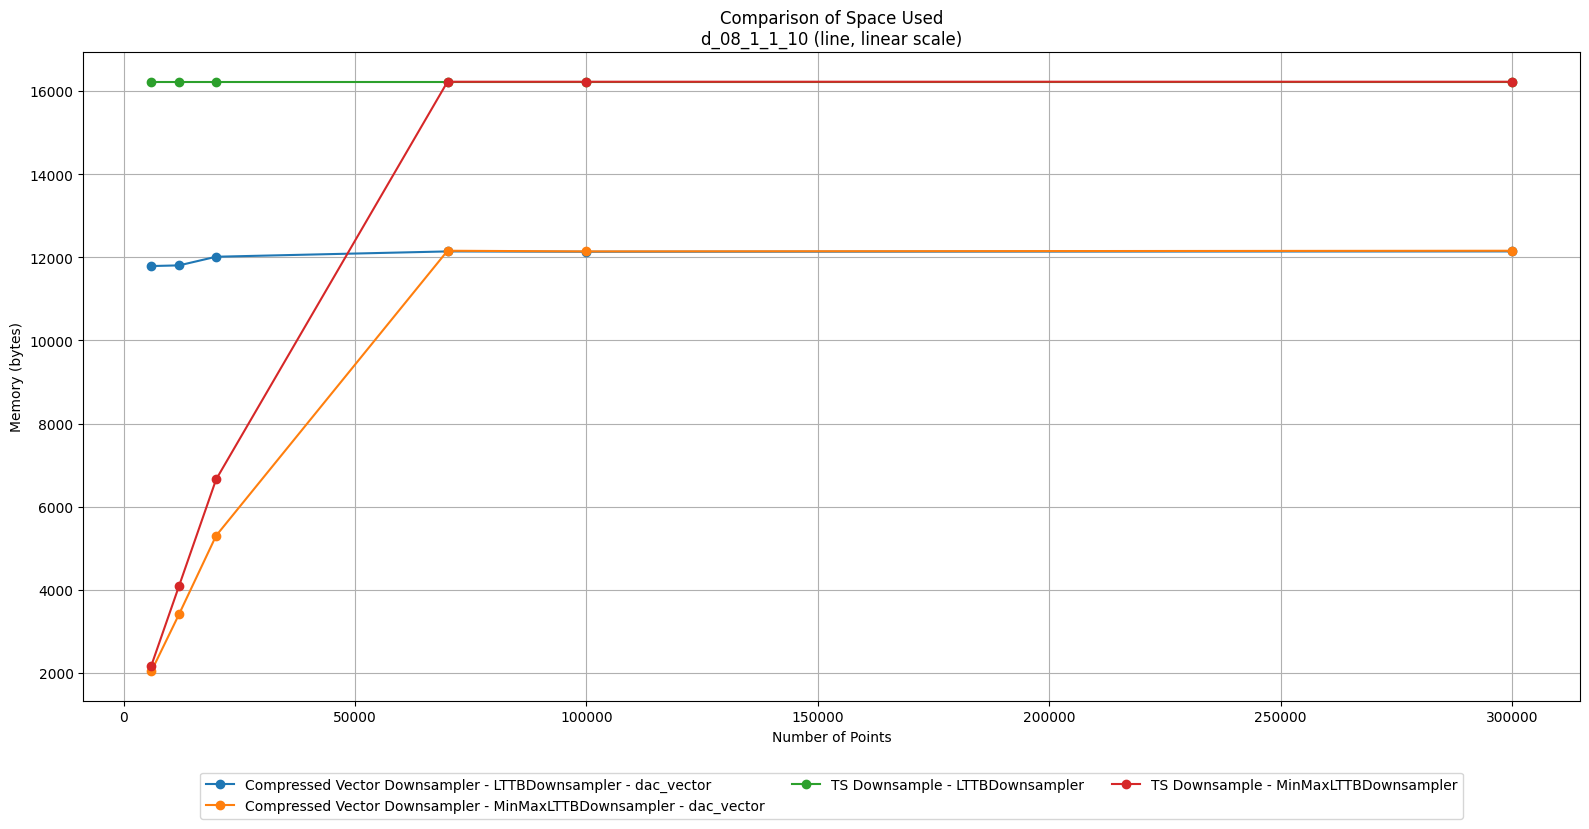
\includegraphics[width=1\textwidth]{anexo/exp/Comparison of Space Used/plots/Comparison of Space Used_d_08_1_1_10_linear_line.png}
        \caption[]{Gráfico de espacio usado por las diferentes bibliotecas para el input \textbf{d\_08\_1\_1\_10}.}
        \label{fig:comparison_of_space_used_plot_line_2}
    \end{figure}
}

\DeclareRobustCommand{\ComparisonOfSpaceUsedTwoPlotBar}{
    %insertar imagen
    \begin{figure}[H]
        \centering
        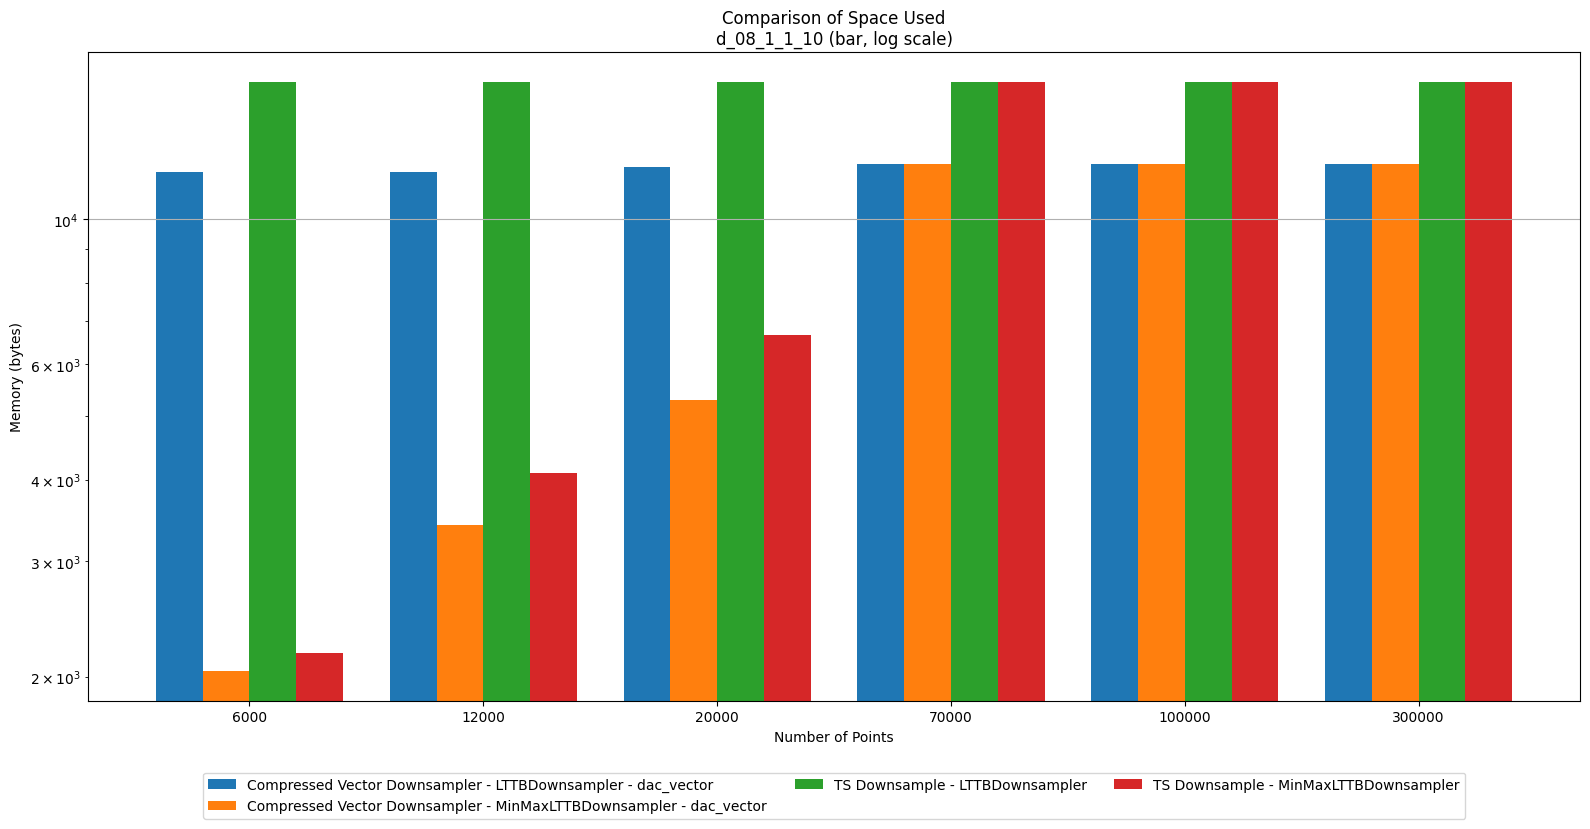
\includegraphics[width=1\textwidth]{anexo/exp/Comparison of Space Used/bar_plots/Comparison of Space Used_d_08_1_1_10_log_bar.png}
        \caption[]{Gráfico de espacio usado por las diferentes bibliotecas para el input \textbf{d\_08\_1\_1\_10}.}
        \label{fig:comparison_of_space_used_plot_bar_2}
    \end{figure}

    \begin{table}[H]
        \centering
        \resizebox{\textwidth}{!}{%
        \begin{tabular}{|l|c|c|c|c|c|c|}
        \hline\multicolumn{1}{|c|}{Option} & \multicolumn{6}{c|}{\textbf{Number of data points}} \\
        \cline{2-7}
         & \textbf{6000} & \textbf{12000} & \textbf{20000} & \textbf{70000} & \textbf{100000} & \textbf{300000} \\
        \hline
        Compressed Vector Downsample - dac\_vector & 1.67e+03 [B] & 2.73e+03 [B] & 4.21e+03 [B] & 9.57e+03 [B] & 9.55e+03 [B] & 9.57e+03 [B] \\
        Compressed Vector Downsample - vlc\_vector\_fibonacci & 1.28e+03 [B] & 2.33e+03 [B] & 3.77e+03 [B] & 9.15e+03 [B] & 9.13e+03 [B] & 9.17e+03 [B] \\
        Original Data & 1.06e+05 [B] & 2.16e+05 [B] & 3.46e+05 [B] & 1.12e+06 [B] & 1.60e+06 [B] & 5.20e+06 [B] \\
        TS Downsample & 2.18e+03 [B] & 4.10e+03 [B] & 6.66e+03 [B] & 1.62e+04 [B] & 1.62e+04 [B] & 1.62e+04 [B] \\
        \hline
        \end{tabular}
        }
        \label{tab:comparison of space used-d-08-1-1-10}
    \end{table}
        \begin{table}[H]
\centering
\caption{Comparison of Space Used\_d\_08\_1\_1\_10 – Tasa de compactación CVD vs TS vs Datos Originales}
\label{tab:Comparison of Space Used\_d\_08\_1\_1\_10_cvd_compactacion}
\begin{tabular}{rlrr}
\toprule
n\_size & Variante & Comp. vs TS (\%) & Comp. vs Original (\%) \\
\midrule
6000 & CVD - dac\_vector & 23.25 & 98.43 \\
6000 & CVD - vlc\_vector\_fibonacci & 41.27 & 98.80 \\
12000 & CVD - dac\_vector & 33.45 & 98.74 \\
12000 & CVD - vlc\_vector\_fibonacci & 43.02 & 98.92 \\
20000 & CVD - dac\_vector & 36.81 & 98.78 \\
20000 & CVD - vlc\_vector\_fibonacci & 43.42 & 98.91 \\
70000 & CVD - dac\_vector & 41.04 & 99.15 \\
70000 & CVD - vlc\_vector\_fibonacci & 43.60 & 99.19 \\
100000 & CVD - dac\_vector & 41.14 & 99.40 \\
100000 & CVD - vlc\_vector\_fibonacci & 43.75 & 99.43 \\
300000 & CVD - dac\_vector & 41.04 & 99.82 \\
300000 & CVD - vlc\_vector\_fibonacci & 43.45 & 99.82 \\
\bottomrule
\end{tabular}

\end{table}
}

\DeclareRobustCommand{\ComparisonOfSpaceUsedThreePlotLine}{
    %insertar imagen
    \begin{figure}[H]
        \centering
        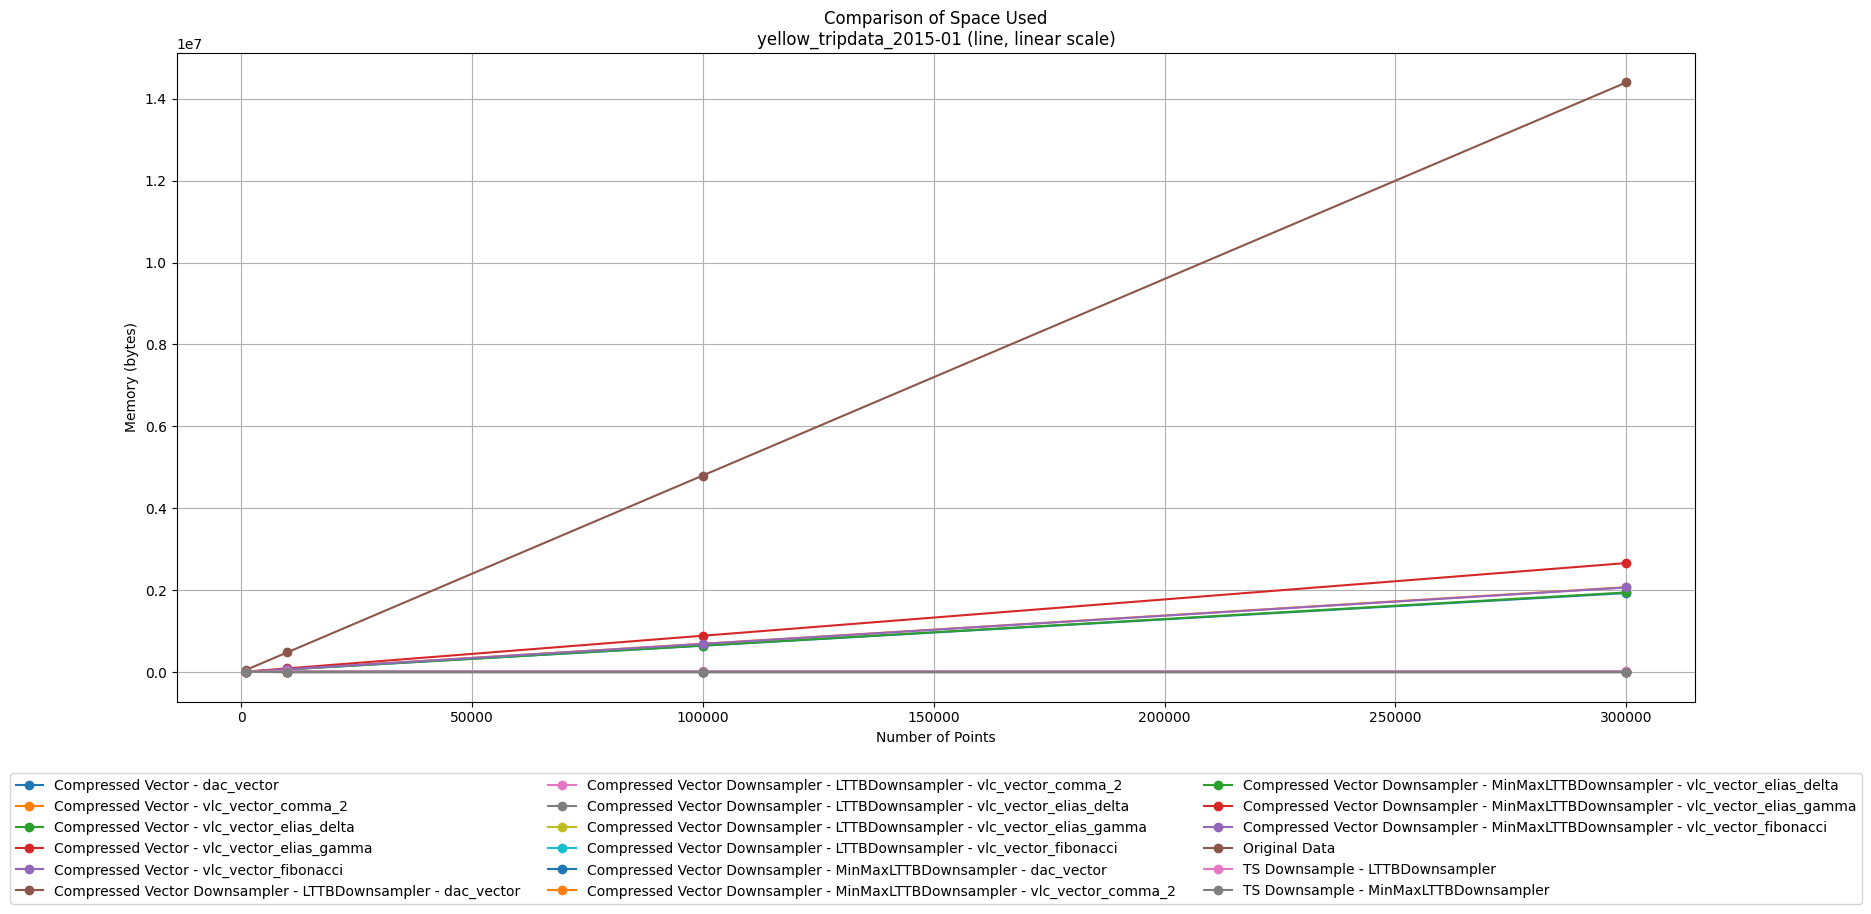
\includegraphics[width=1\textwidth]{anexo/exp/Comparison of Space Used/plots/Comparison of Space Used_yellow_tripdata_2015-01_linear_line.png}
        \caption[]{Gráfico de espacio usado por las diferentes bibliotecas para el input \textbf{yellow\_tripdata\_2015\_01}.}
        \label{fig:comparison_of_space_used_plot_line_3}
    \end{figure}
}

\DeclareRobustCommand{\ComparisonOfSpaceUsedThreePlotBar}{
    %insertar imagen
    \begin{figure}[H]
        \centering
        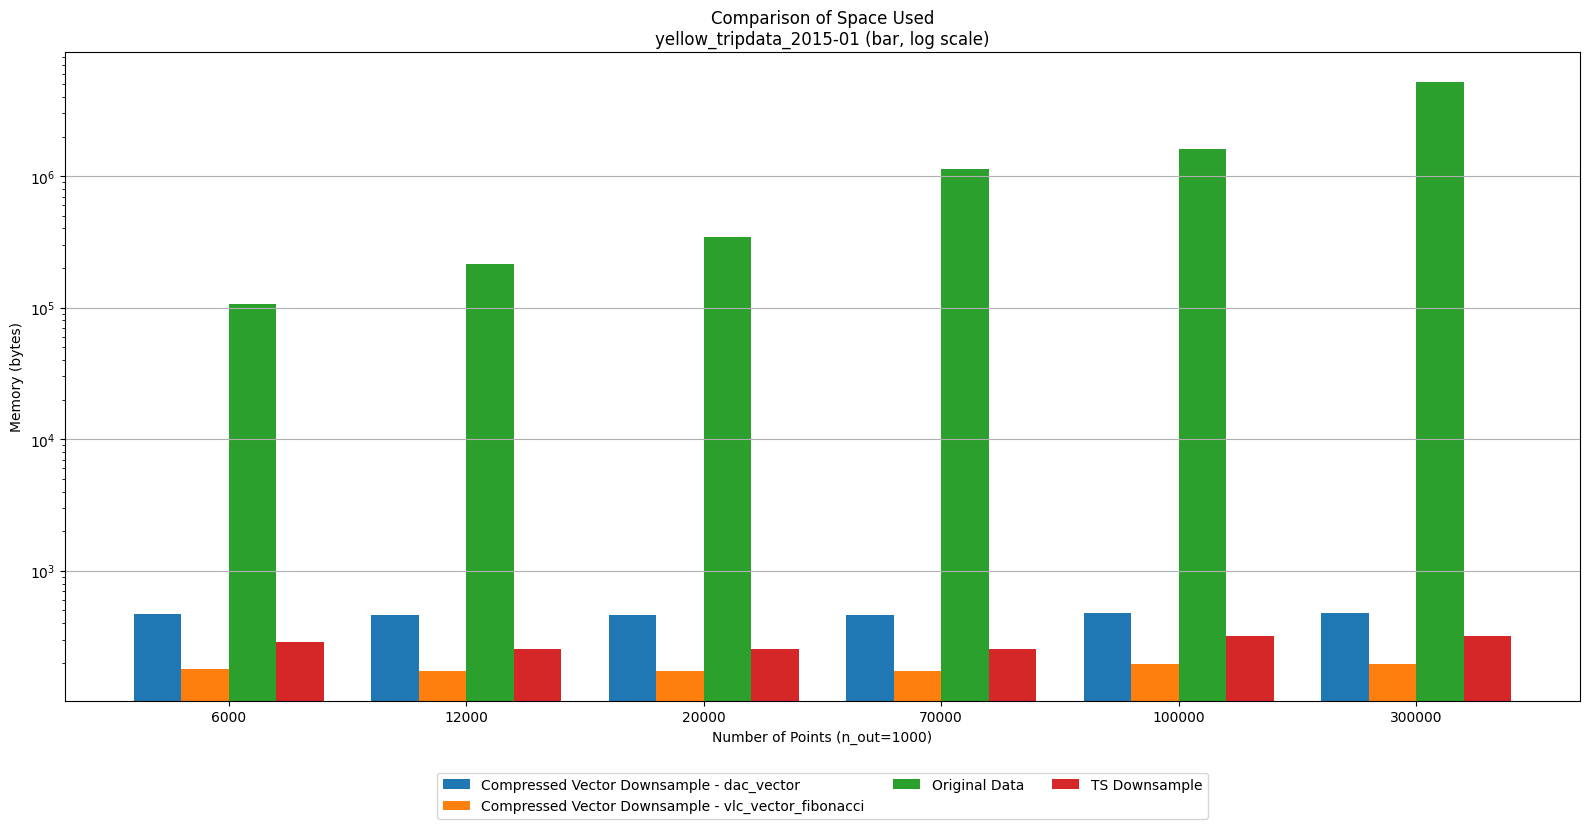
\includegraphics[width=1\textwidth]{anexo/exp/Comparison of Space Used/bar_plots/Comparison of Space Used_yellow_tripdata_2015-01_log_bar.png}
        \caption[]{Gráfico de espacio usado por las diferentes bibliotecas para el input \textbf{yellow\_tripdata\_2015\_01}.}
        \label{fig:comparison_of_space_used_plot_bar_3}
    \end{figure}
    \begin{table}[H]
        \centering
        \resizebox{\textwidth}{!}{%
        \begin{tabular}{|l|c|c|c|c|c|c|}
        \hline\multicolumn{1}{|c|}{Option} & \multicolumn{6}{c|}{\textbf{Number of data points}} \\
        \cline{2-7}
         & \textbf{6000} & \textbf{12000} & \textbf{20000} & \textbf{70000} & \textbf{100000} & \textbf{300000} \\
        \hline
        Compressed Vector Downsample - dac\_vector & 4.68e+02 [B] & 4.60e+02 [B] & 4.60e+02 [B] & 4.60e+02 [B] & 4.76e+02 [B] & 4.76e+02 [B] \\
        Compressed Vector Downsample - vlc\_vector\_fibonacci & 1.80e+02 [B] & 1.72e+02 [B] & 1.72e+02 [B] & 1.72e+02 [B] & 1.96e+02 [B] & 1.96e+02 [B] \\
        Original Data & 1.06e+05 [B] & 2.16e+05 [B] & 3.46e+05 [B] & 1.12e+06 [B] & 1.60e+06 [B] & 5.20e+06 [B] \\
        TS Downsample & 2.88e+02 [B] & 2.56e+02 [B] & 2.56e+02 [B] & 2.56e+02 [B] & 3.20e+02 [B] & 3.20e+02 [B] \\
        \hline
        \end{tabular}
        }
        \label{tab:comparison of space used-yellow-tripdata-2015-01}
    \end{table}
    \begin{table}[H]
\centering
\caption{Comparison of Space Used\_yellow\_tripdata\_2015-01 – Tasa de compactación CVD vs TS vs Datos Originales}
\label{tab:Comparison of Space Used\_yellow\_tripdata\_2015-01_cvd_compactacion}
\begin{tabular}{rlrr}
\toprule
n\_size & Variante & Comp. vs TS (\%) & Comp. vs Original (\%) \\
\midrule
6000 & CVD - dac\_vector & -62.50 & 99.56 \\
6000 & CVD - vlc\_vector\_fibonacci & 37.50 & 99.83 \\
12000 & CVD - dac\_vector & -79.69 & 99.79 \\
12000 & CVD - vlc\_vector\_fibonacci & 32.81 & 99.92 \\
20000 & CVD - dac\_vector & -79.69 & 99.87 \\
20000 & CVD - vlc\_vector\_fibonacci & 32.81 & 99.95 \\
70000 & CVD - dac\_vector & -79.69 & 99.96 \\
70000 & CVD - vlc\_vector\_fibonacci & 32.81 & 99.98 \\
100000 & CVD - dac\_vector & -48.75 & 99.97 \\
100000 & CVD - vlc\_vector\_fibonacci & 38.75 & 99.99 \\
300000 & CVD - dac\_vector & -48.75 & 99.99 \\
300000 & CVD - vlc\_vector\_fibonacci & 38.75 & 100.00 \\
\bottomrule
\end{tabular}

\end{table}
}



% ===========================
% CVD Decimal Places Access Time Comparison
% ===========================
\DeclareRobustCommand{\CVDDecimalPlacesAccessTimeComparisonOnePlotLine}{
    \begin{figure}[H]
        \centering
        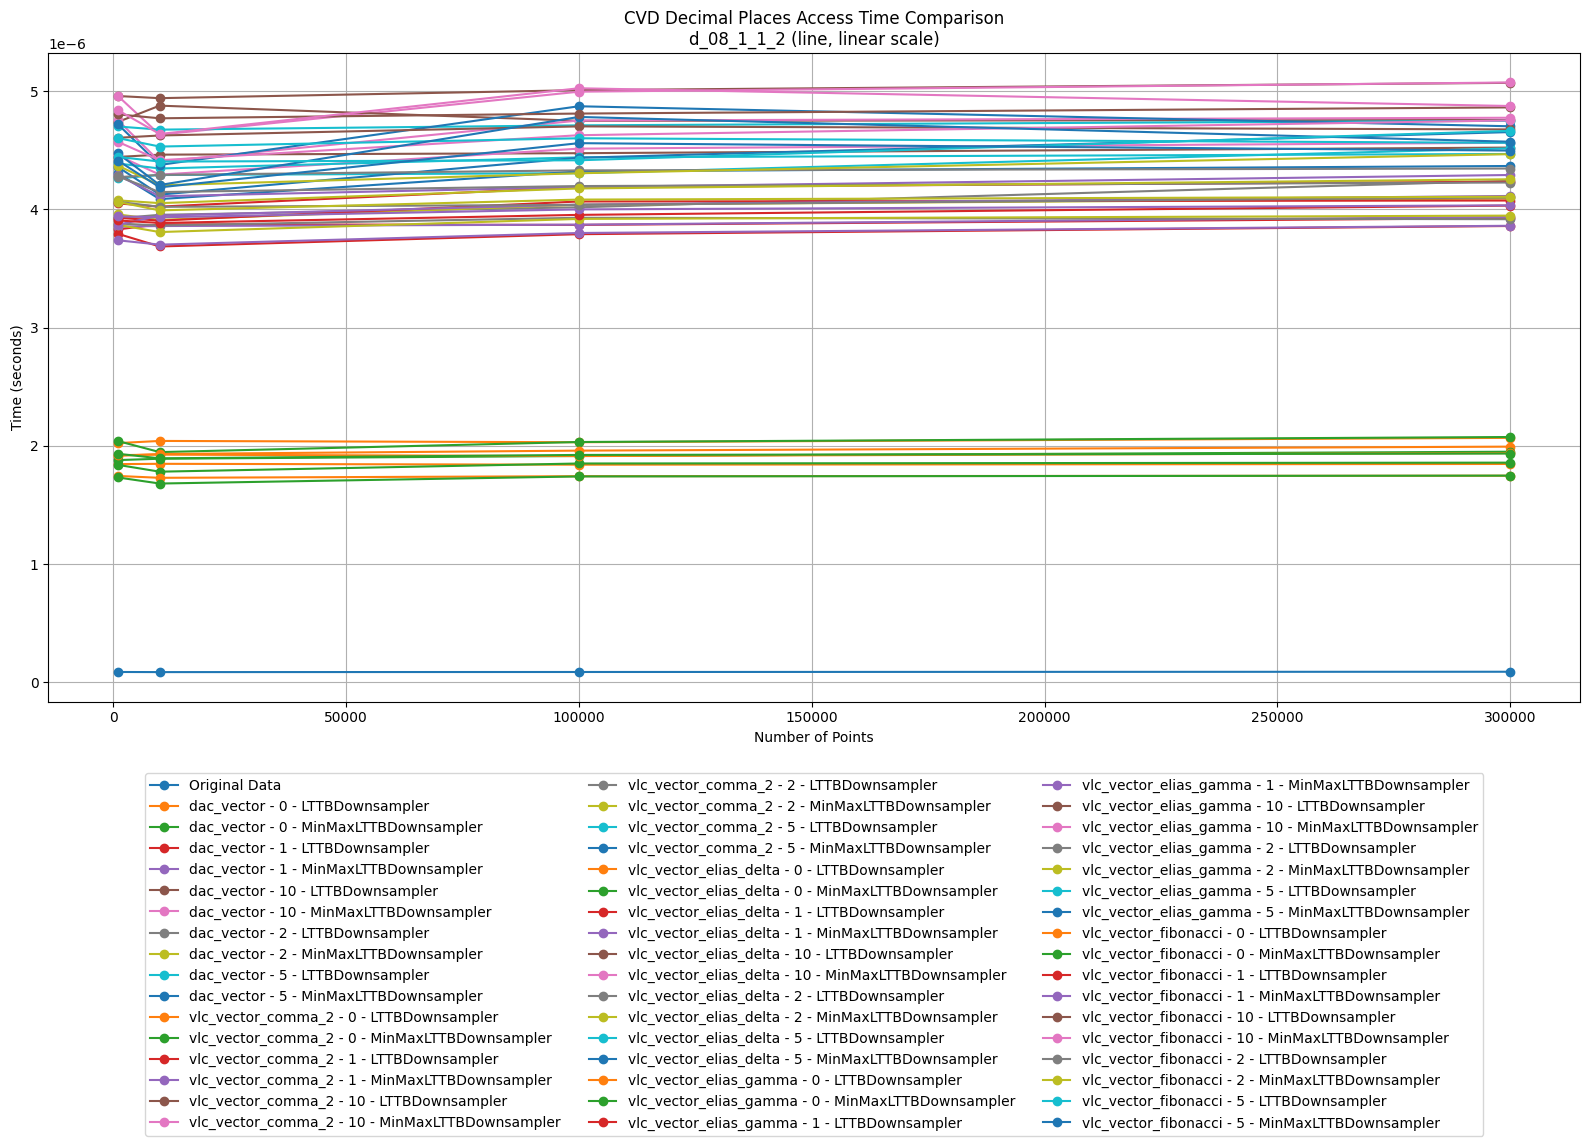
\includegraphics[width=1\textwidth]{anexo/exp/CVD Decimal Places Access Time Comparison/plots/CVD Decimal Places Access Time Comparison_d_08_1_1_2_linear_line.png}
        \caption[]{Gráfico de tiempo de acceso CVD con diferentes lugares decimales para el input \textbf{d\_08\_1\_1\_2}.}
        \label{fig:cvd_decimal_places_access_time_comparison_plot_line_1}
    \end{figure}
    \begin{figure}[H]
        \centering
        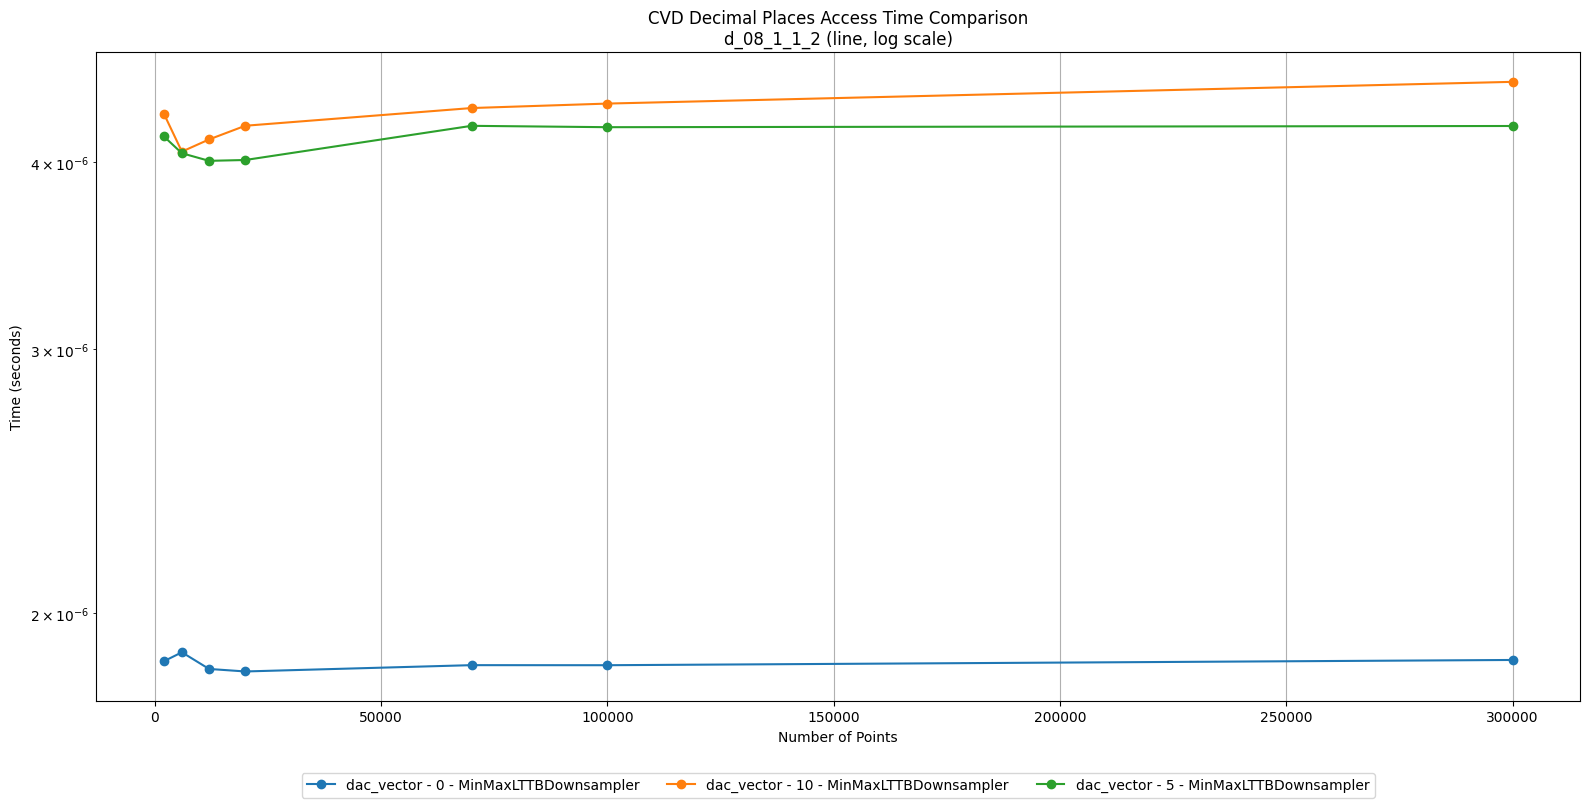
\includegraphics[width=1\textwidth]{anexo/exp/CVD Decimal Places Access Time Comparison/plots/CVD Decimal Places Access Time Comparison_d_08_1_1_2_log_line.png}
        \caption[]{Gráfico de tiempo de acceso CVD con diferentes lugares decimales para el input \textbf{d\_08\_1\_1\_2} en escala logarítmica.}
        \label{fig:cvd_decimal_places_access_time_comparison_plot_log_1}
    \end{figure}
}

\DeclareRobustCommand{\CVDDecimalPlacesAccessTimeComparisonTwoPlotLine}{
    \begin{figure}[H]
        \centering
        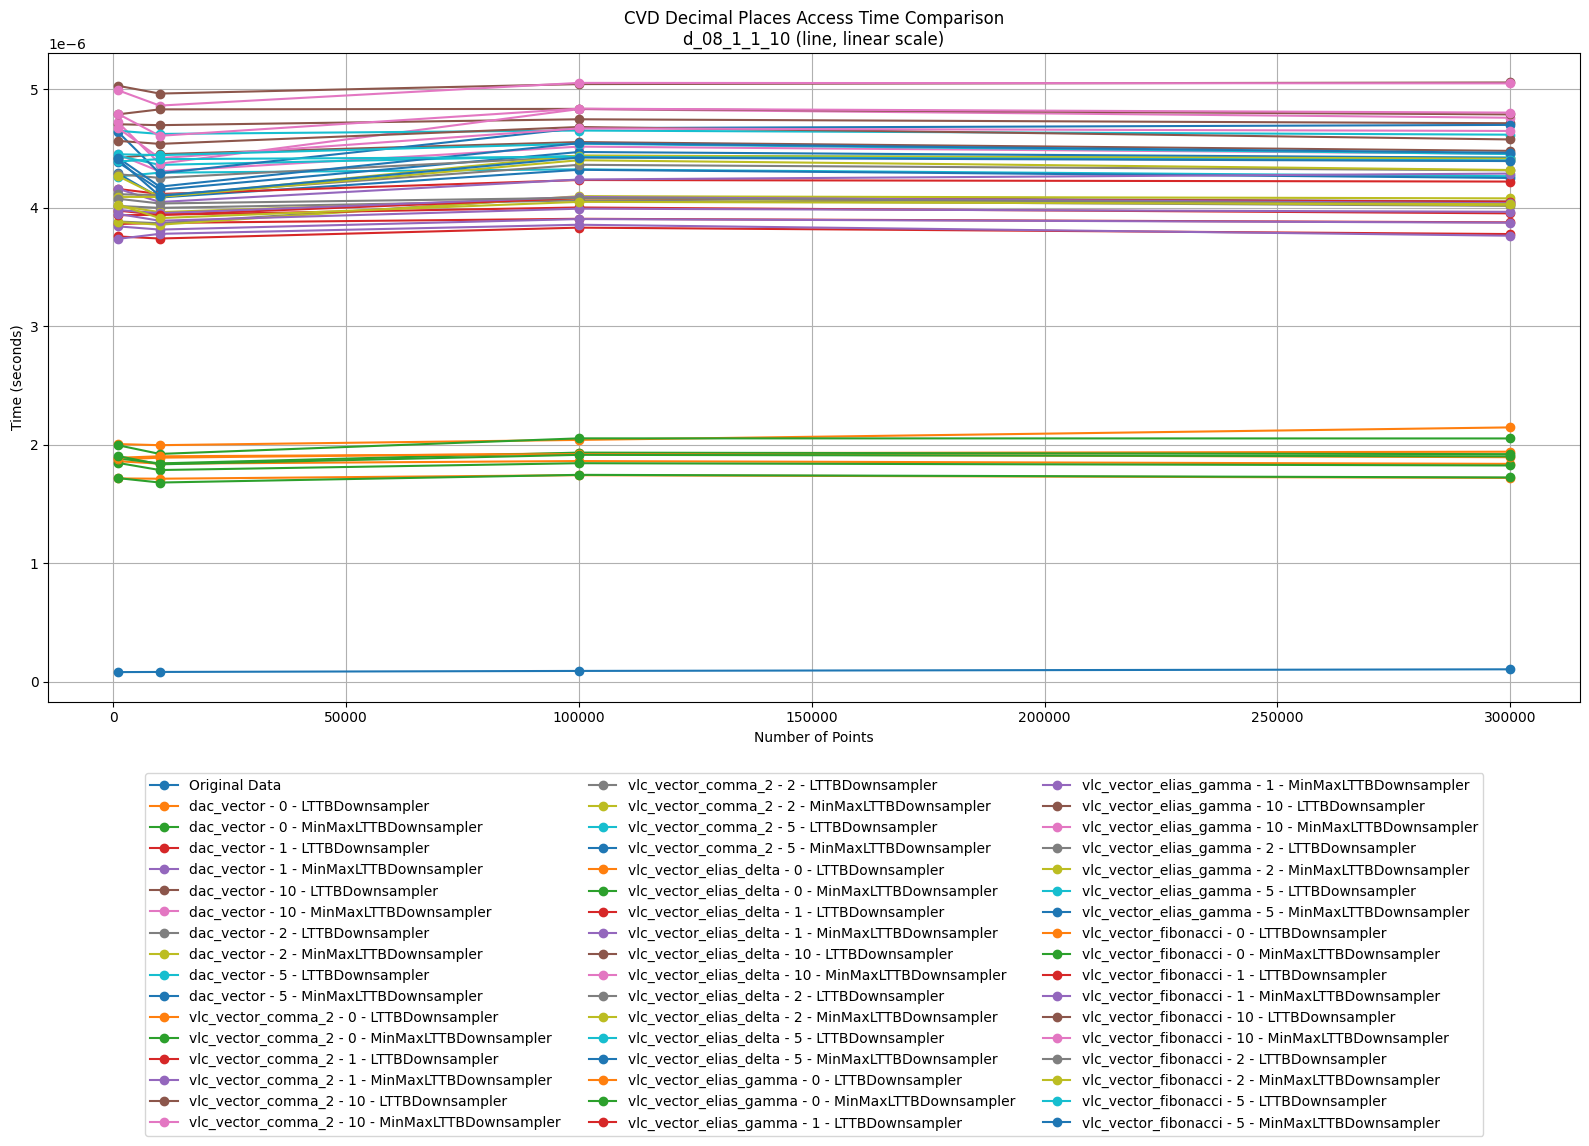
\includegraphics[width=1\textwidth]{anexo/exp/CVD Decimal Places Access Time Comparison/plots/CVD Decimal Places Access Time Comparison_d_08_1_1_10_linear_line.png}
        \caption[]{Gráfico de tiempo de acceso CVD con diferentes lugares decimales para el input \textbf{d\_08\_1\_1\_10}.}
        \label{fig:cvd_decimal_places_access_time_comparison_plot_line_2}
    \end{figure}
    \begin{figure}[H]
        \centering
        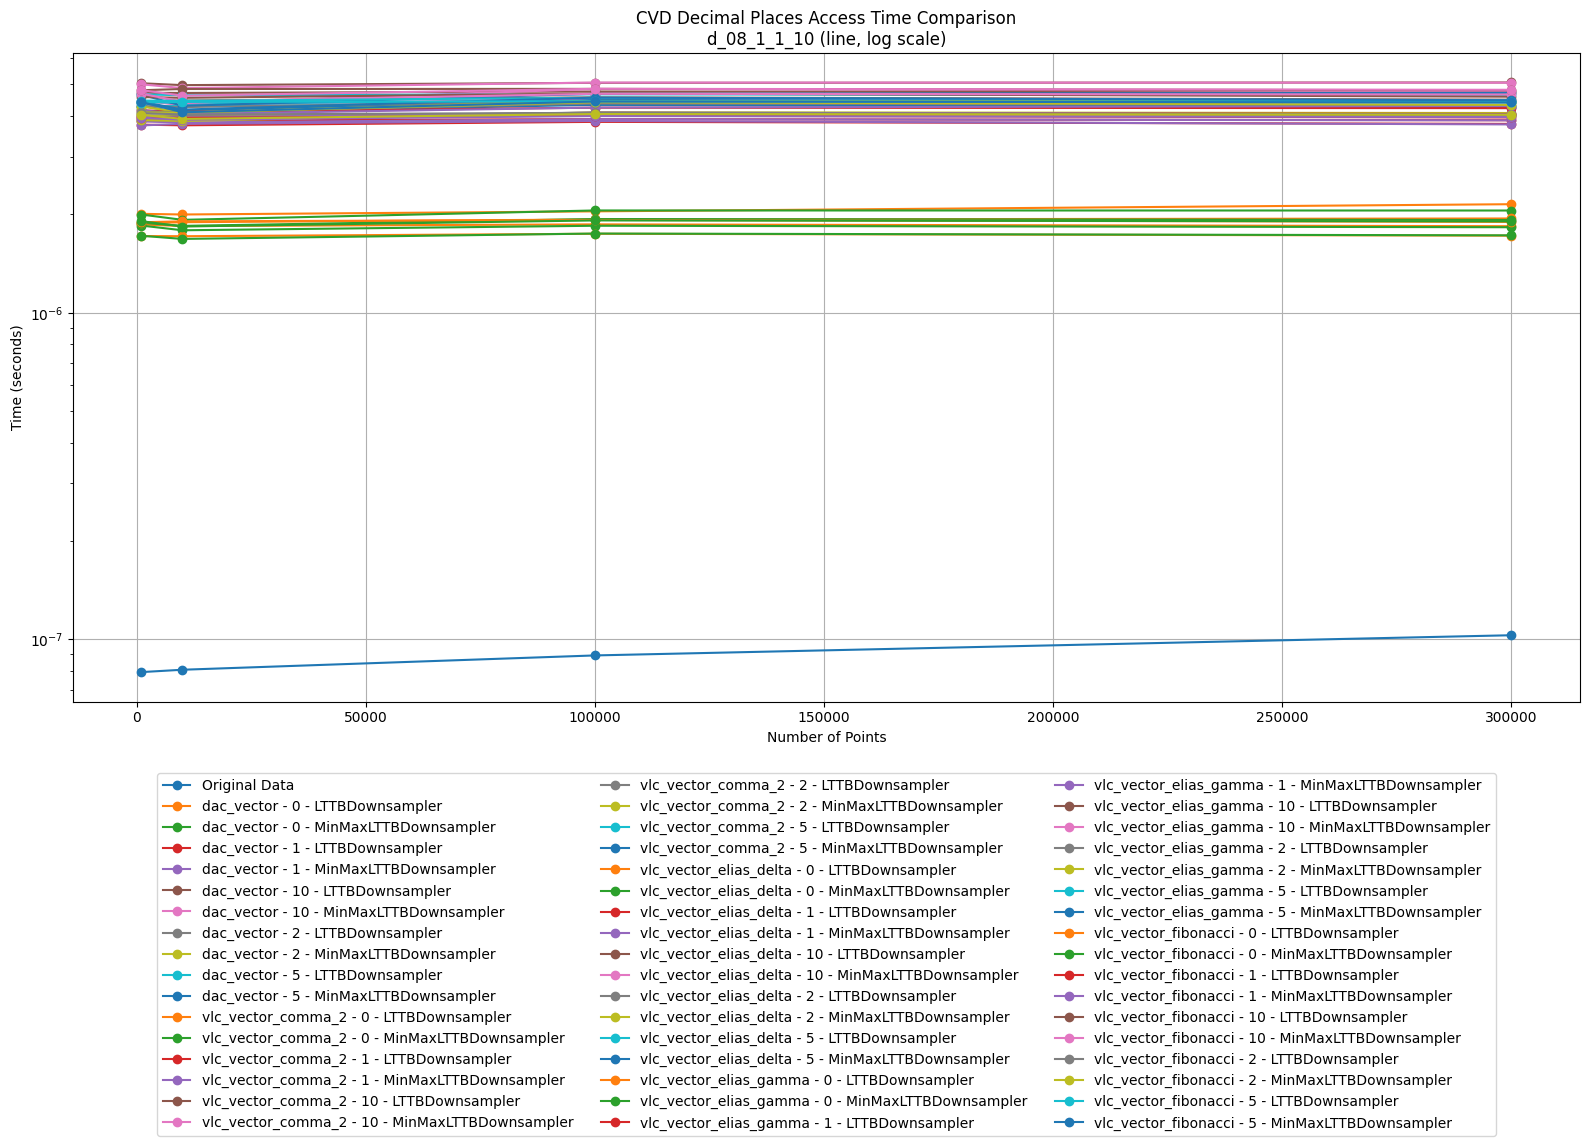
\includegraphics[width=1\textwidth]{anexo/exp/CVD Decimal Places Access Time Comparison/plots/CVD Decimal Places Access Time Comparison_d_08_1_1_10_log_line.png}
        \caption[]{Gráfico de tiempo de acceso CVD con diferentes lugares decimales para el input \textbf{d\_08\_1\_1\_10} en escala logarítmica.}
        \label{fig:cvd_decimal_places_access_time_comparison_plot_log_2}
    \end{figure}
}

\DeclareRobustCommand{\CVDDecimalPlacesAccessTimeComparisonThreePlotLine}{
    \begin{figure}[H]
        \centering
        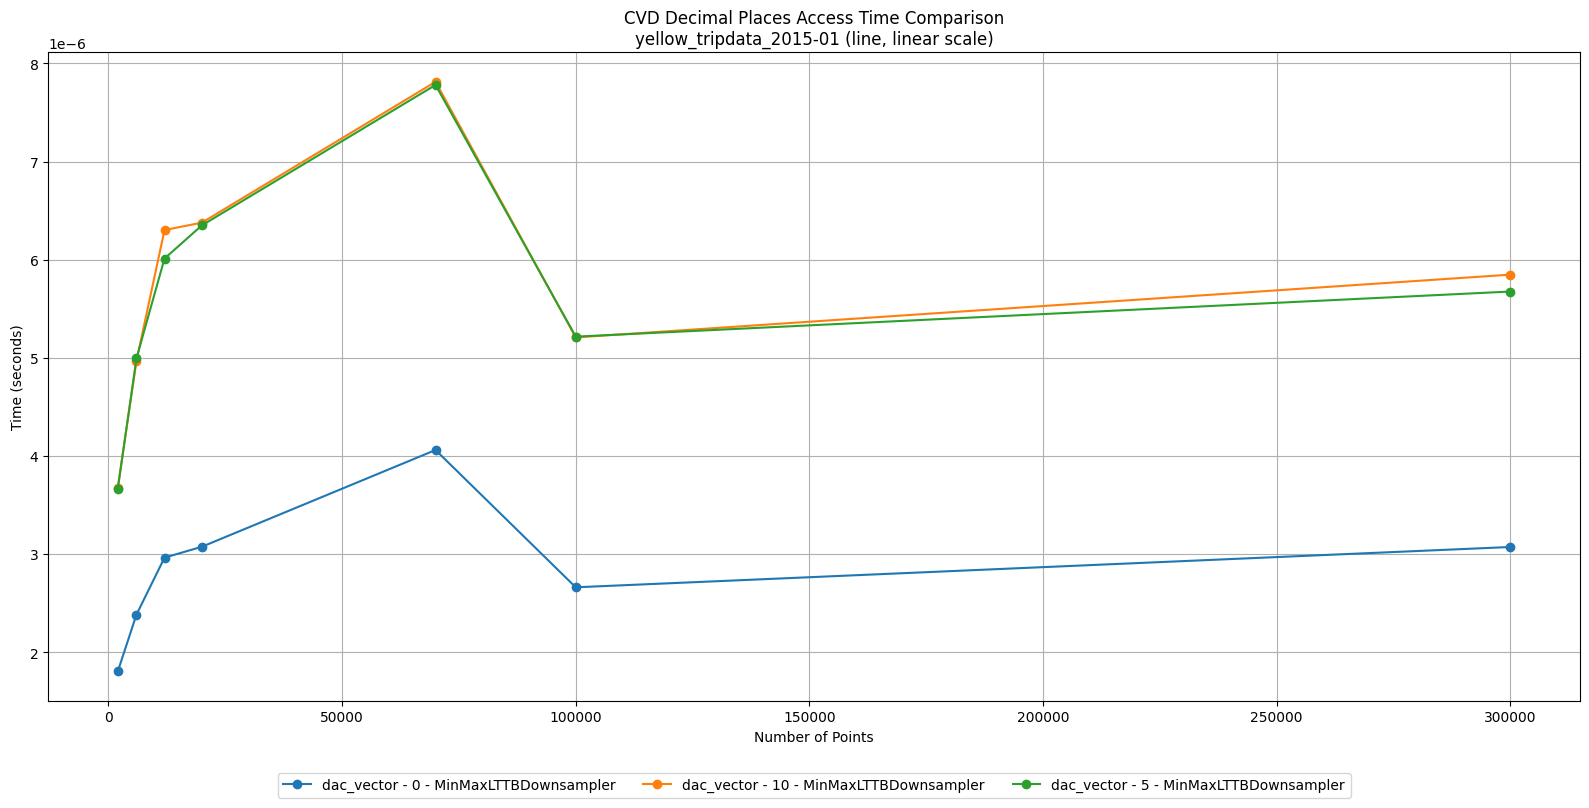
\includegraphics[width=1\textwidth]{anexo/exp/CVD Decimal Places Access Time Comparison/plots/CVD Decimal Places Access Time Comparison_yellow_tripdata_2015-01_linear_line.png}
        \caption[]{Gráfico de tiempo de acceso CVD con diferentes lugares decimales para el input \textbf{yellow\_tripdata\_2015\_01}.}
        \label{fig:cvd_decimal_places_access_time_comparison_plot_line_3}
    \end{figure}
    \begin{figure}[H]
        \centering
        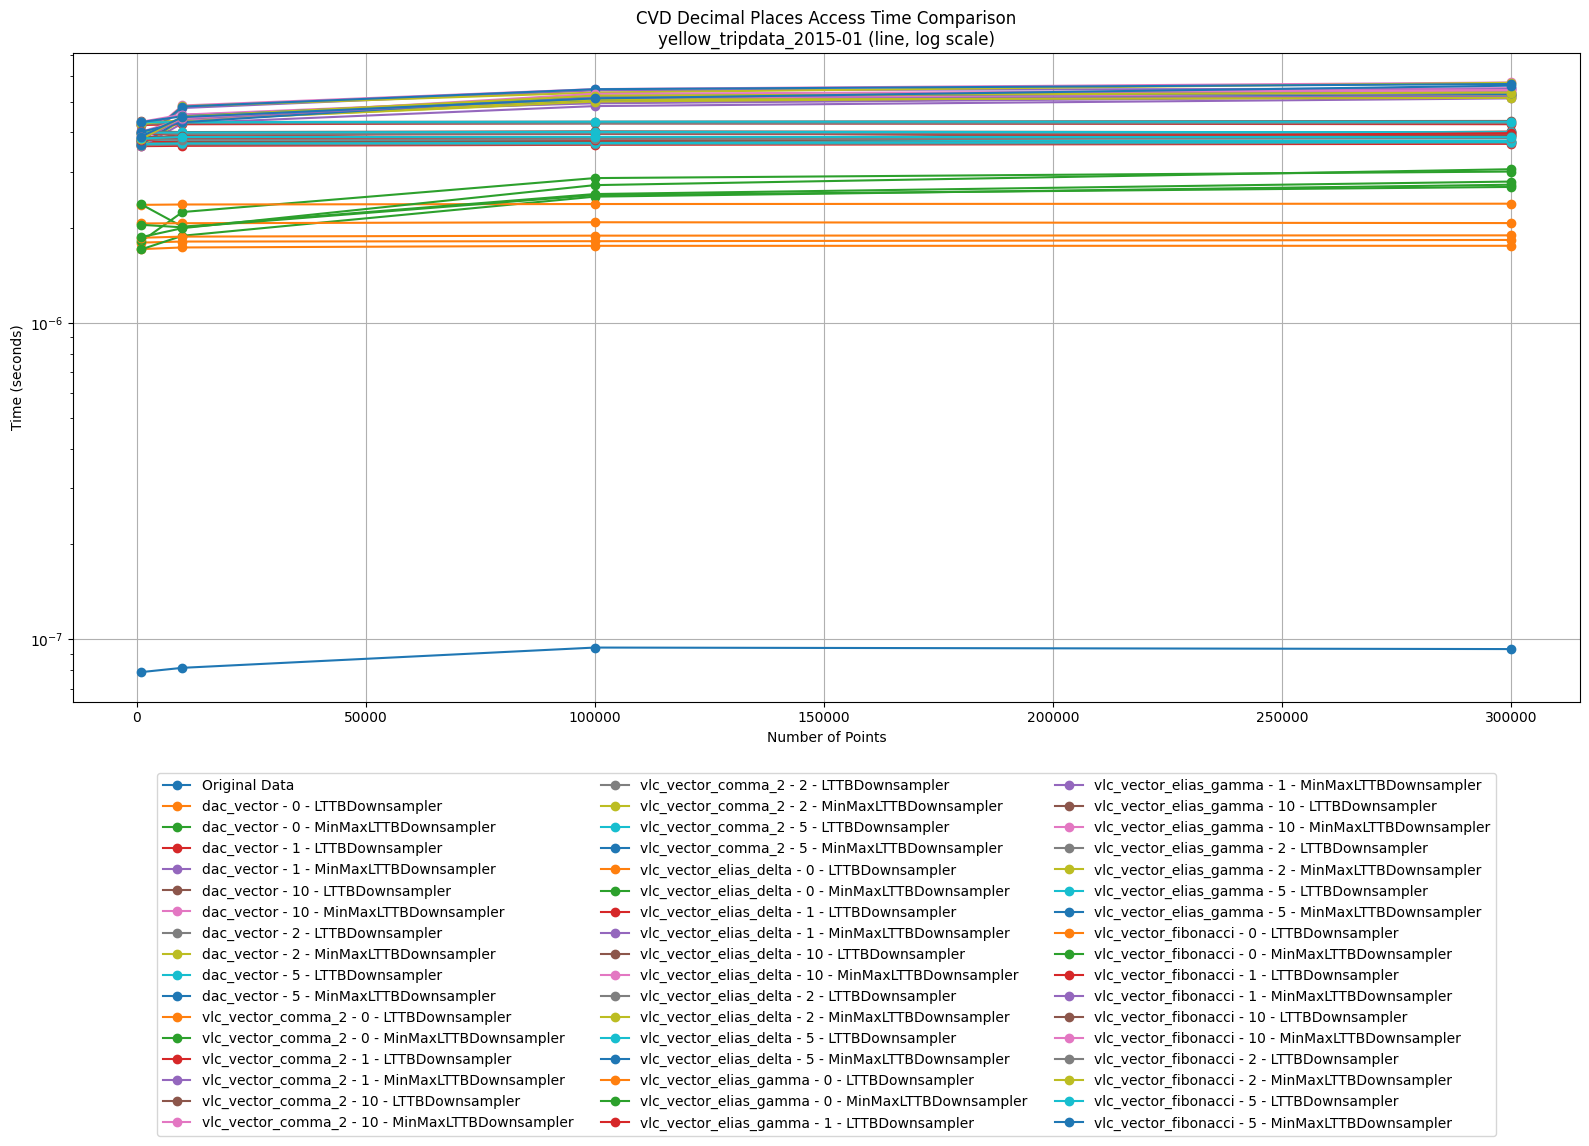
\includegraphics[width=1\textwidth]{anexo/exp/CVD Decimal Places Access Time Comparison/plots/CVD Decimal Places Access Time Comparison_yellow_tripdata_2015-01_log_line.png}
        \caption[]{Gráfico de tiempo de acceso CVD con diferentes lugares decimales para el input \textbf{yellow\_tripdata\_2015\_01} en escala logarítmica.}
        \label{fig:cvd_decimal_places_access_time_comparison_plot_log_3}
    \end{figure}
}


% ===========================
% CVD Decimal Places Build Time Comparison
% ===========================
\DeclareRobustCommand{\CVDDecimalPlacesBuildTimeComparisonOnePlotLine}{
    \begin{figure}[H]
        \centering
        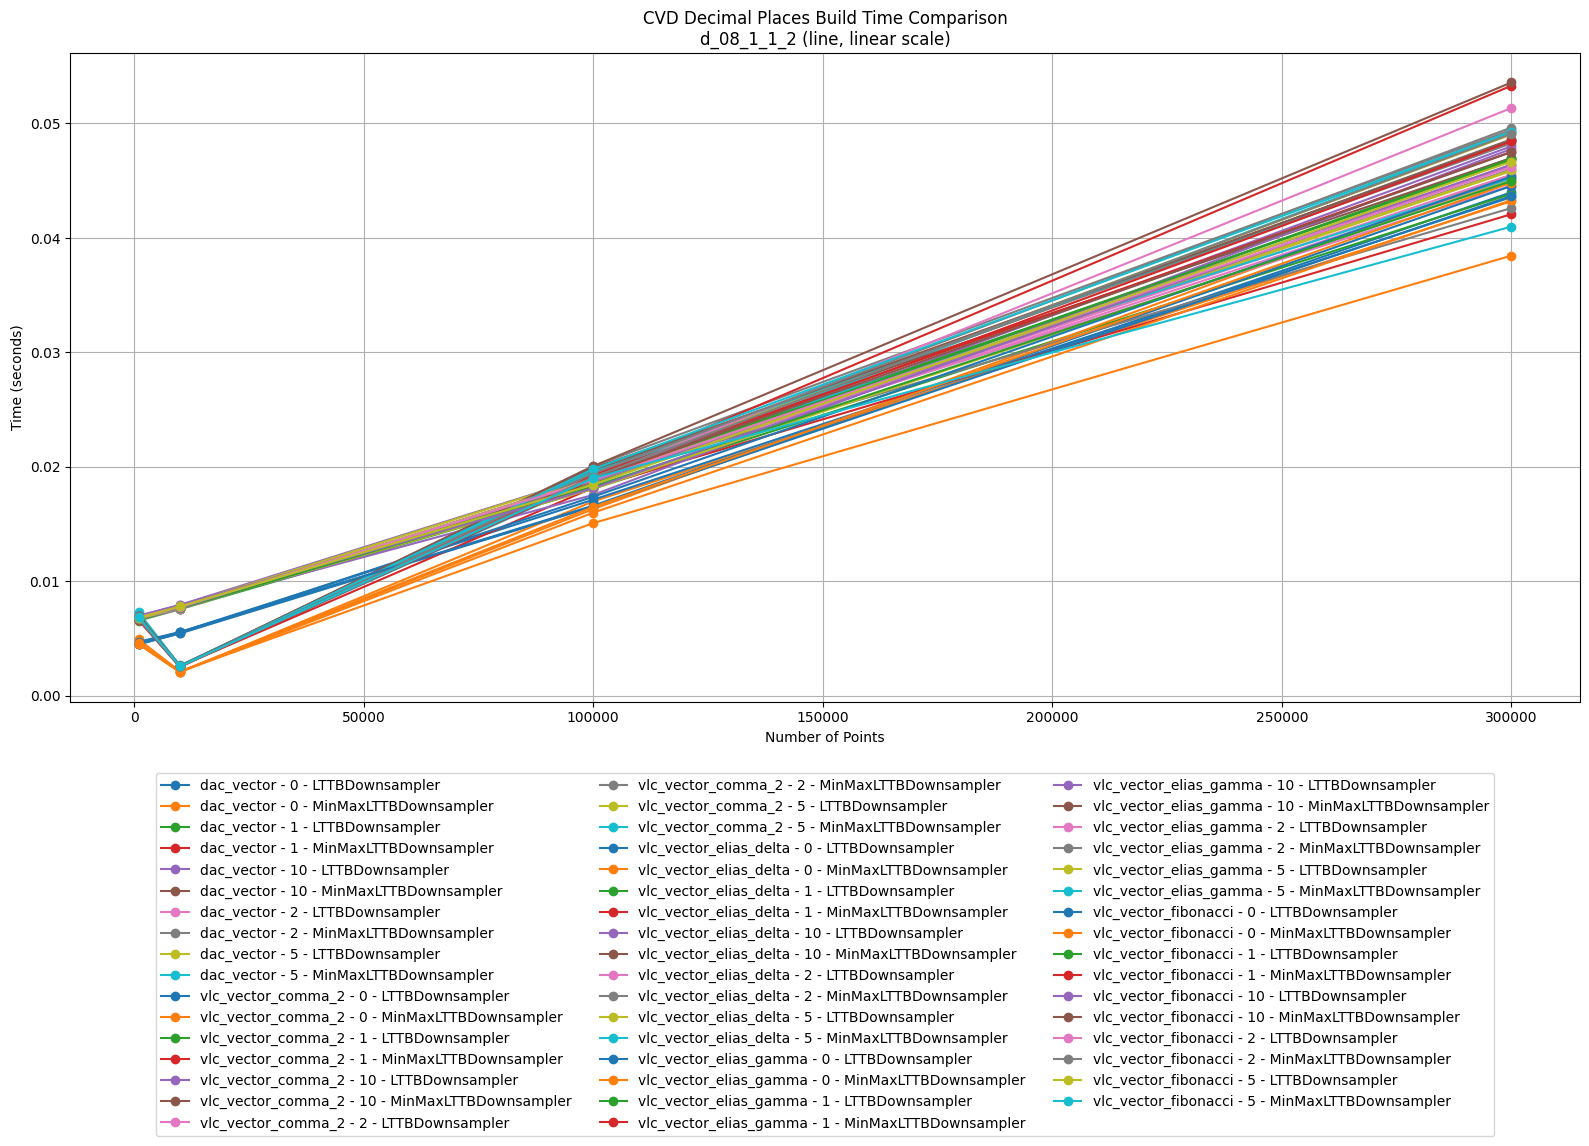
\includegraphics[width=1\textwidth]{anexo/exp/CVD Decimal Places Build Time Comparison/plots/CVD Decimal Places Build Time Comparison_d_08_1_1_2_linear_line.png}
        \caption[]{Gráfico de tiempo de construcción CVD con diferentes lugares decimales para el input \textbf{d\_08\_1\_1\_2}.}
        \label{fig:cvd_decimal_places_build_time_comparison_plot_line_1}
    \end{figure}
    \begin{figure}[H]
        \centering
        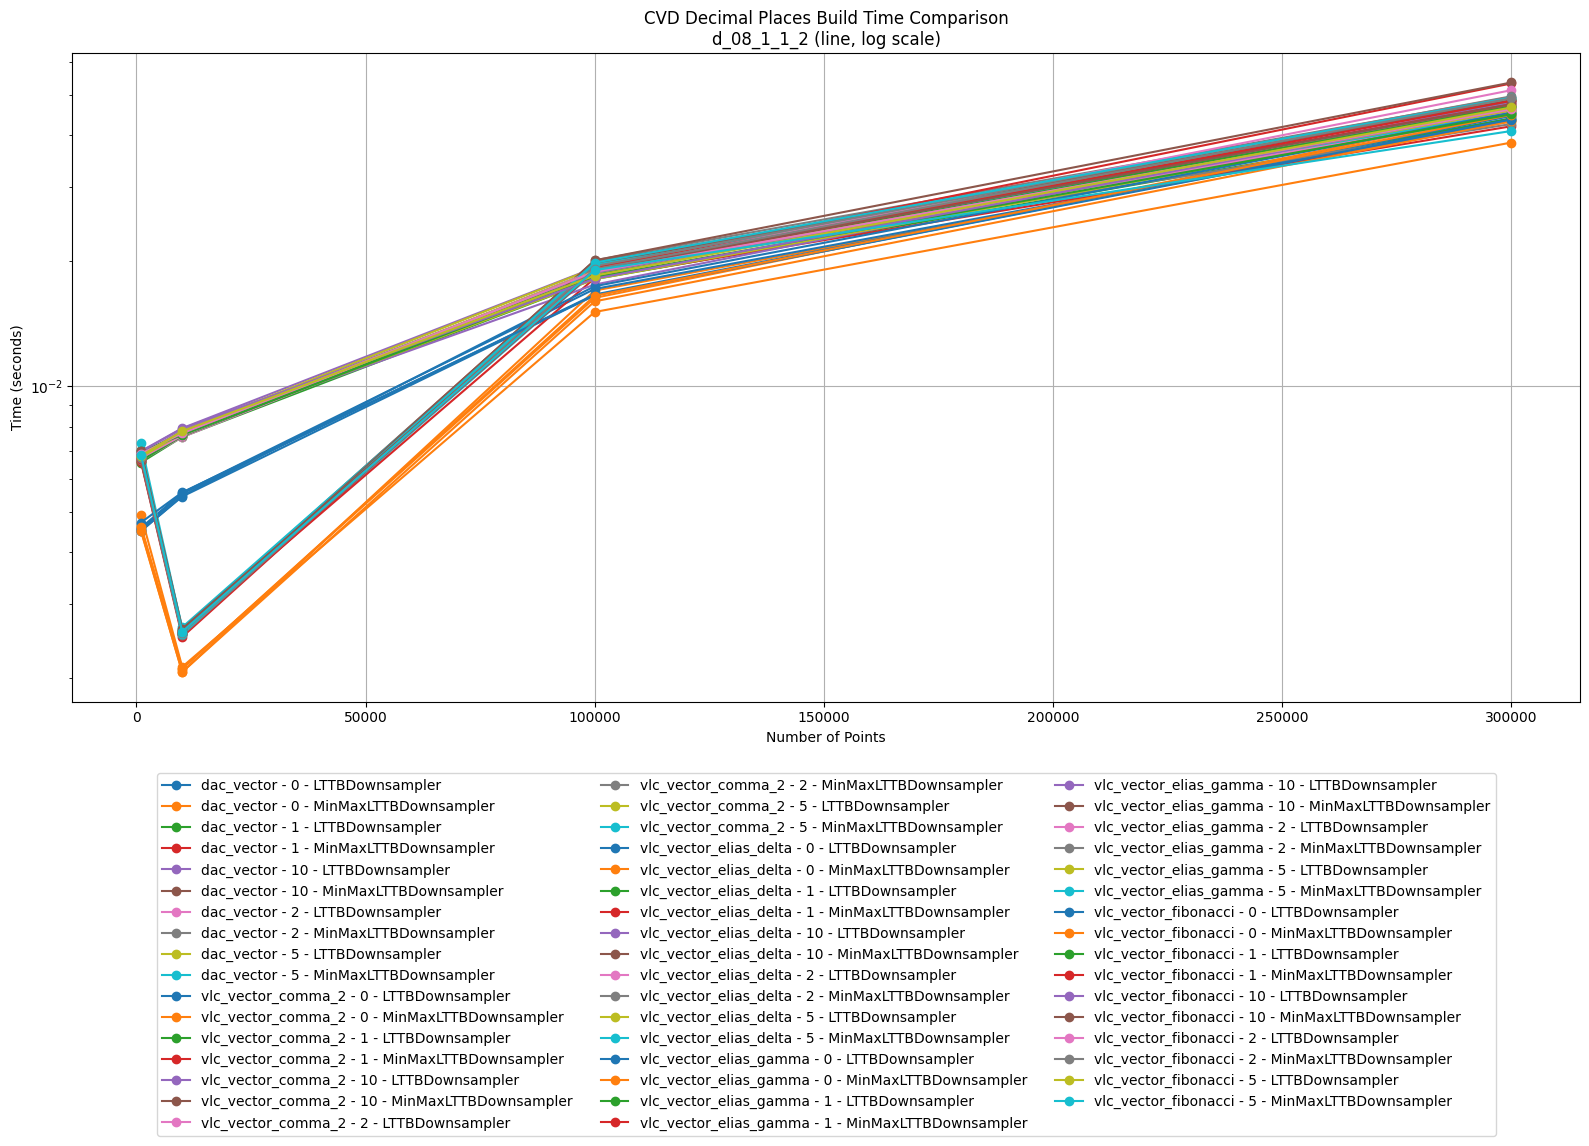
\includegraphics[width=1\textwidth]{anexo/exp/CVD Decimal Places Build Time Comparison/plots/CVD Decimal Places Build Time Comparison_d_08_1_1_2_log_line.png}
        \caption[]{Gráfico de tiempo de construcción CVD con diferentes lugares decimales para el input \textbf{d\_08\_1\_1\_2} en escala logarítmica.}
        \label{fig:cvd_decimal_places_build_time_comparison_plot_log_1}
    \end{figure}
}

\DeclareRobustCommand{\CVDDecimalPlacesBuildTimeComparisonTwoPlotLine}{
    \begin{figure}[H]
        \centering
        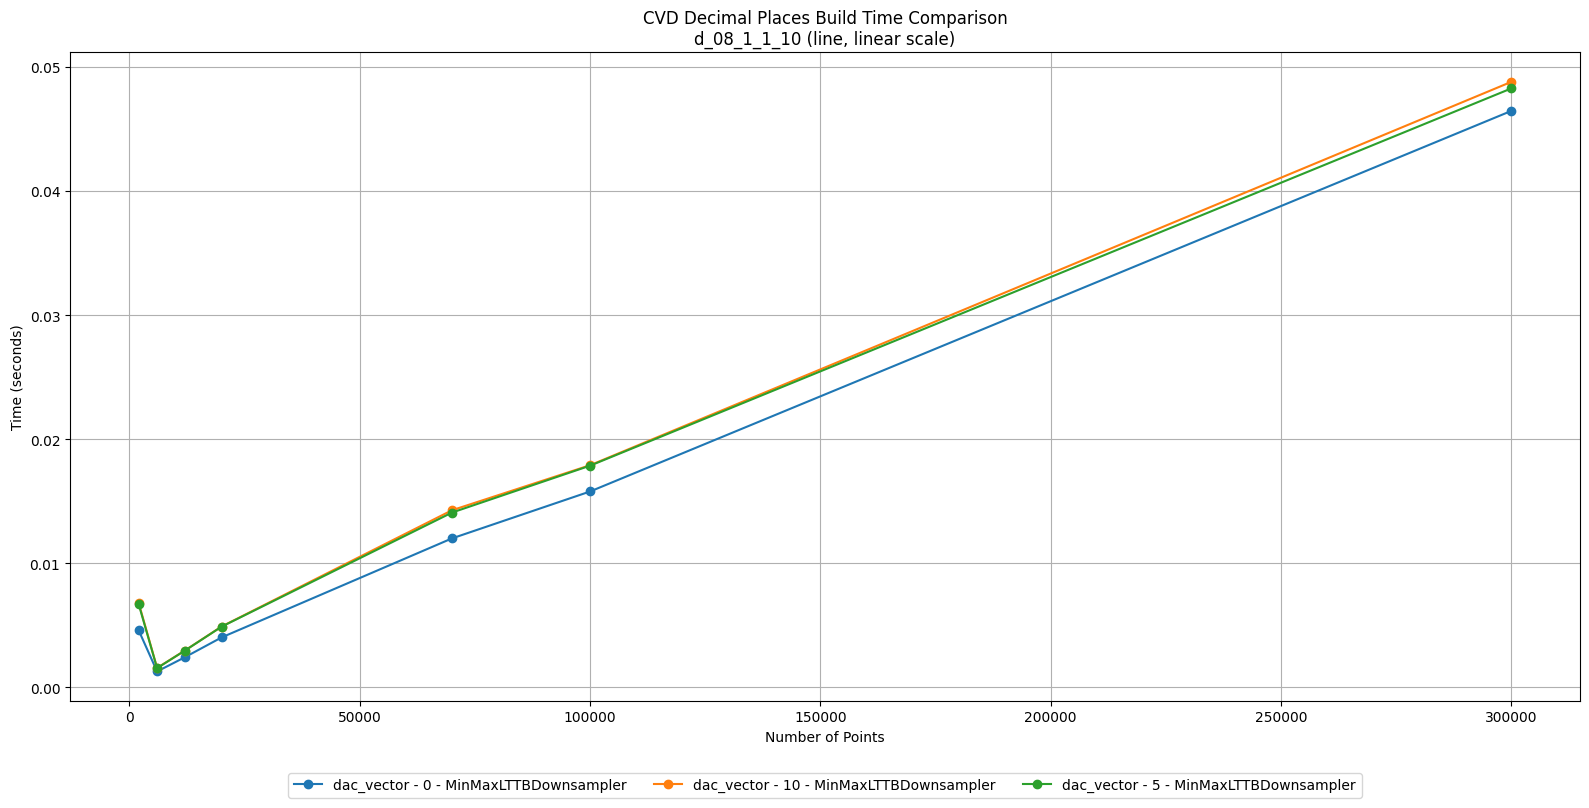
\includegraphics[width=1\textwidth]{anexo/exp/CVD Decimal Places Build Time Comparison/plots/CVD Decimal Places Build Time Comparison_d_08_1_1_10_linear_line.png}
        \caption[]{Gráfico de tiempo de construcción CVD con diferentes lugares decimales para el input \textbf{d\_08\_1\_1\_10}.}
        \label{fig:cvd_decimal_places_build_time_comparison_plot_line_2}
    \end{figure}
    \begin{figure}[H]
        \centering
        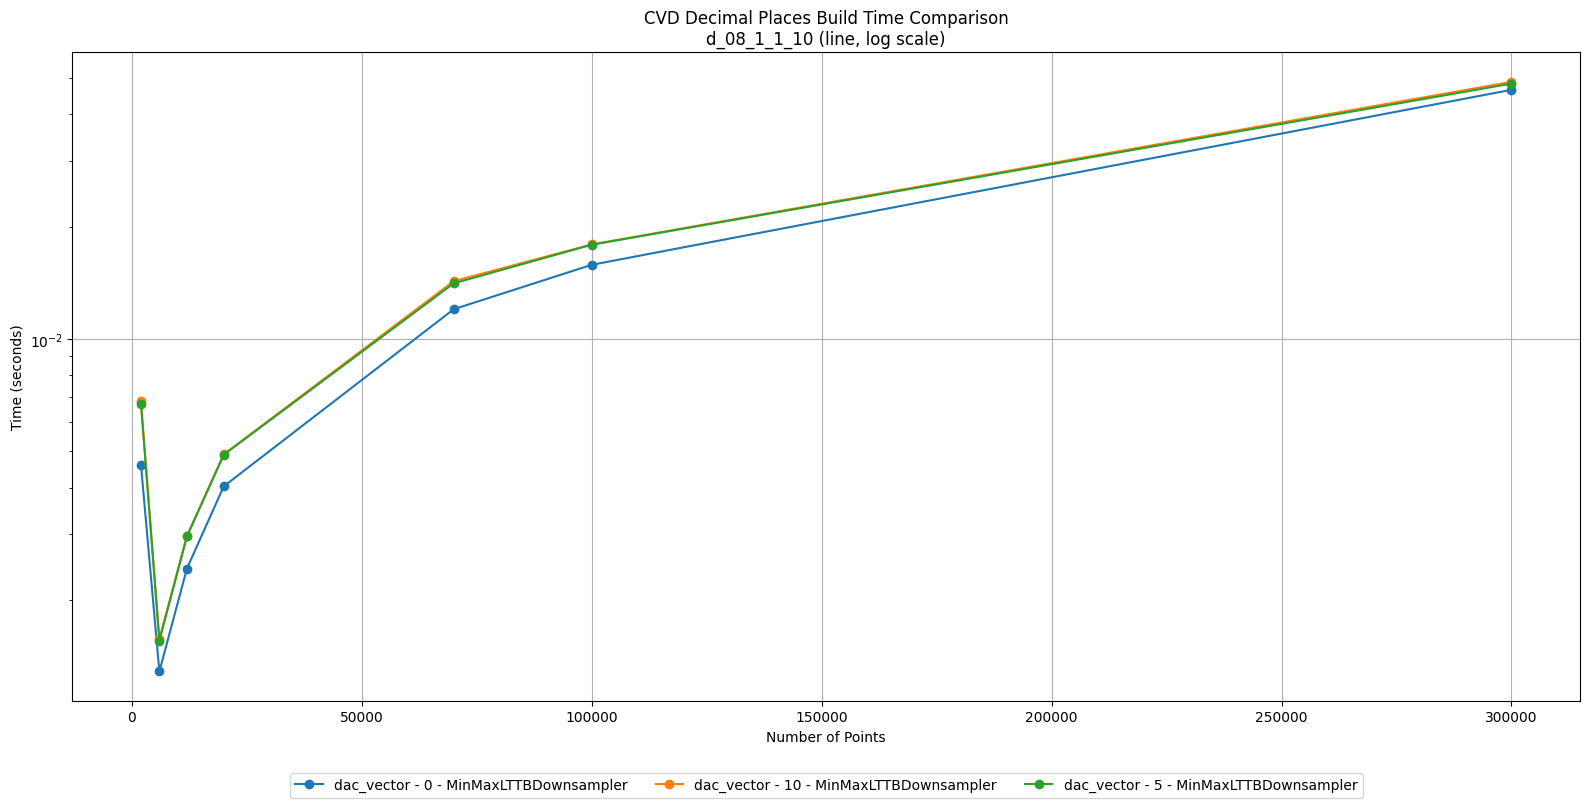
\includegraphics[width=1\textwidth]{anexo/exp/CVD Decimal Places Build Time Comparison/plots/CVD Decimal Places Build Time Comparison_d_08_1_1_10_log_line.png}
        \caption[]{Gráfico de tiempo de construcción CVD con diferentes lugares decimales para el input \textbf{d\_08\_1\_1\_10} en escala logarítmica.}
        \label{fig:cvd_decimal_places_build_time_comparison_plot_log_2}
    \end{figure}
}

\DeclareRobustCommand{\CVDDecimalPlacesBuildTimeComparisonThreePlotLine}{
    \begin{figure}[H]
        \centering
        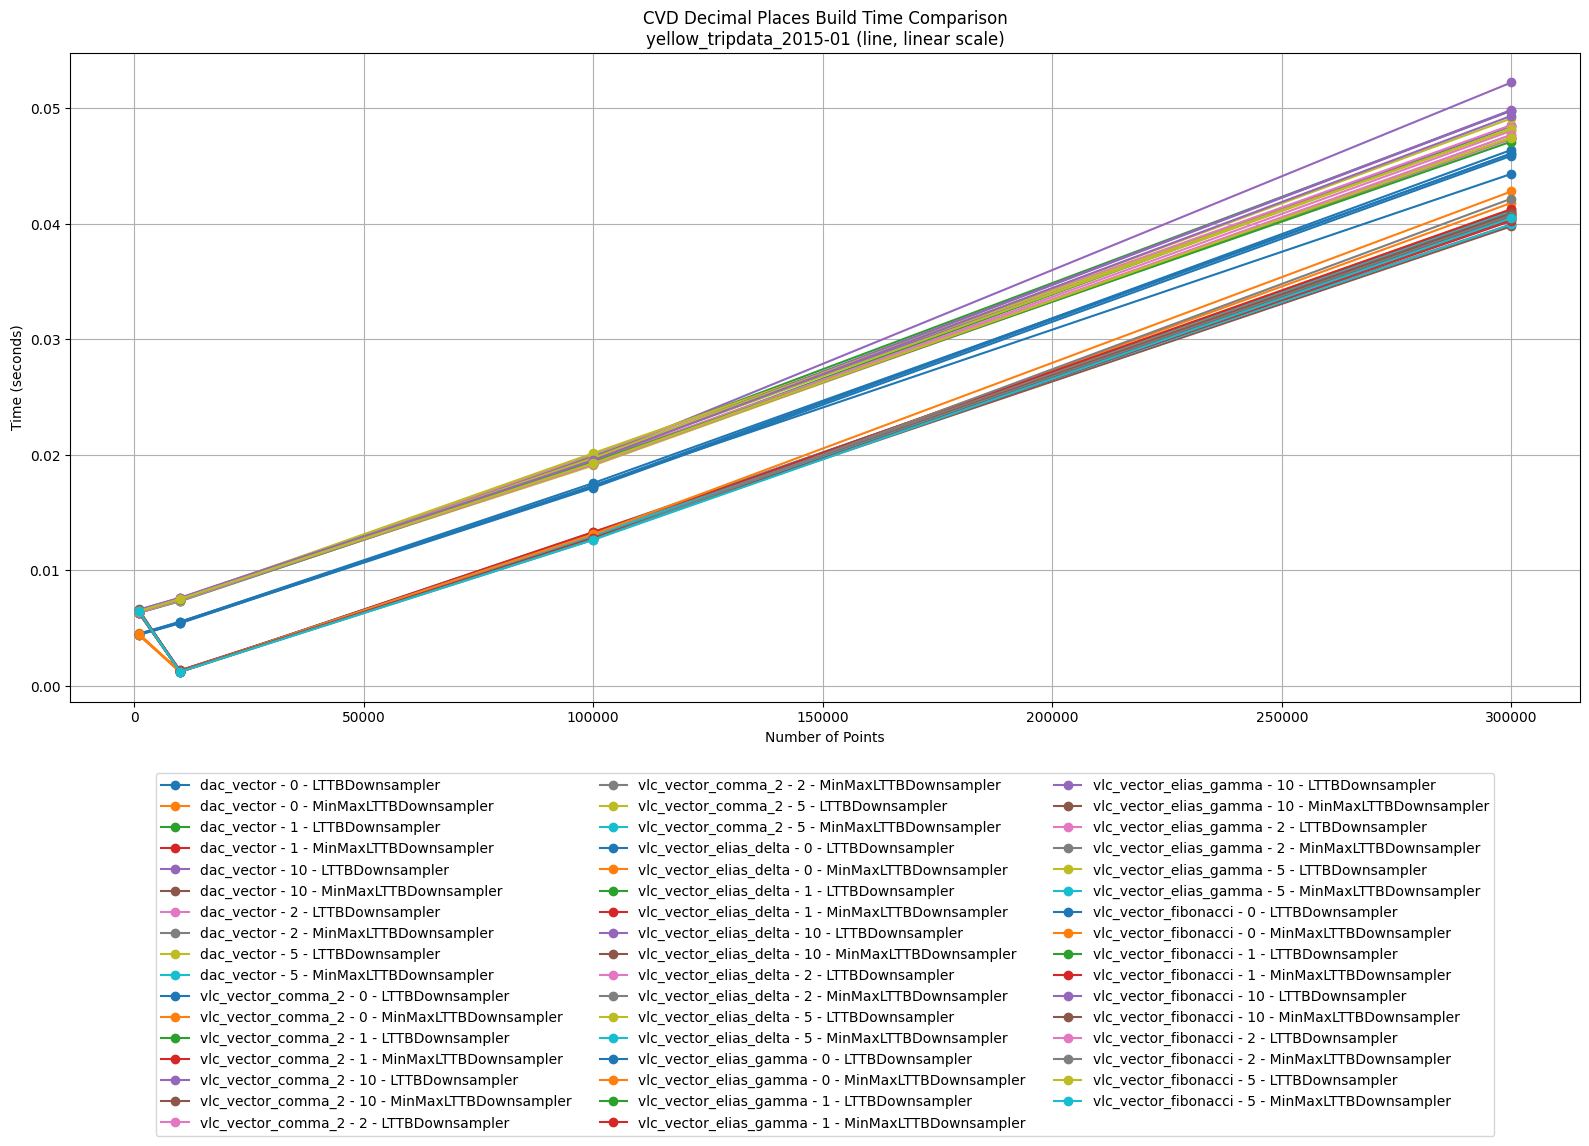
\includegraphics[width=1\textwidth]{anexo/exp/CVD Decimal Places Build Time Comparison/plots/CVD Decimal Places Build Time Comparison_yellow_tripdata_2015-01_linear_line.png}
        \caption[]{Gráfico de tiempo de construcción CVD con diferentes lugares decimales para el input \textbf{yellow\_tripdata\_2015\_01}.}
        \label{fig:cvd_decimal_places_build_time_comparison_plot_line_3}
    \end{figure}
    \begin{figure}[H]
        \centering
        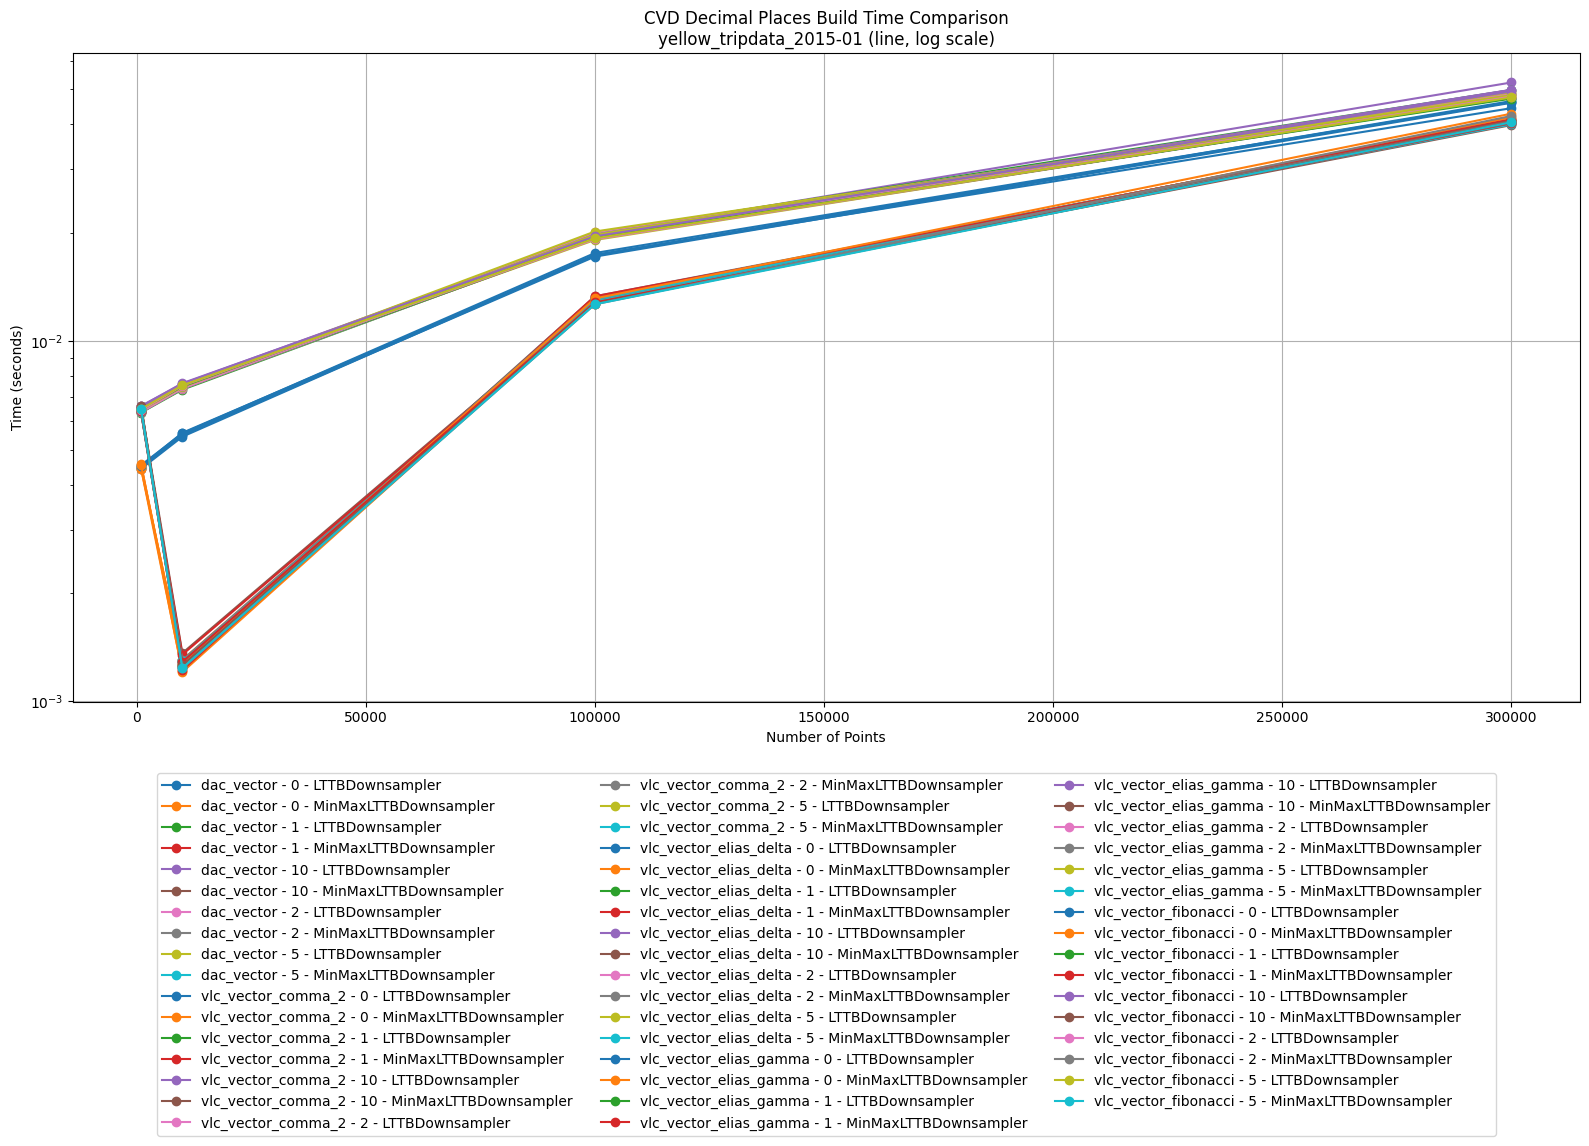
\includegraphics[width=1\textwidth]{anexo/exp/CVD Decimal Places Build Time Comparison/plots/CVD Decimal Places Build Time Comparison_yellow_tripdata_2015-01_log_line.png}
        \caption[]{Gráfico de tiempo de construcción CVD con diferentes lugares decimales para el input \textbf{yellow\_tripdata\_2015\_01} en escala logarítmica.}
        \label{fig:cvd_decimal_places_build_time_comparison_plot_log_3}
    \end{figure}
}


% ===========================
% CVD Decimal Places Size Comparison
% ===========================
\DeclareRobustCommand{\CVDDecimalPlacesSizeComparisonOnePlotLine}{
    \begin{figure}[H]
        \centering
        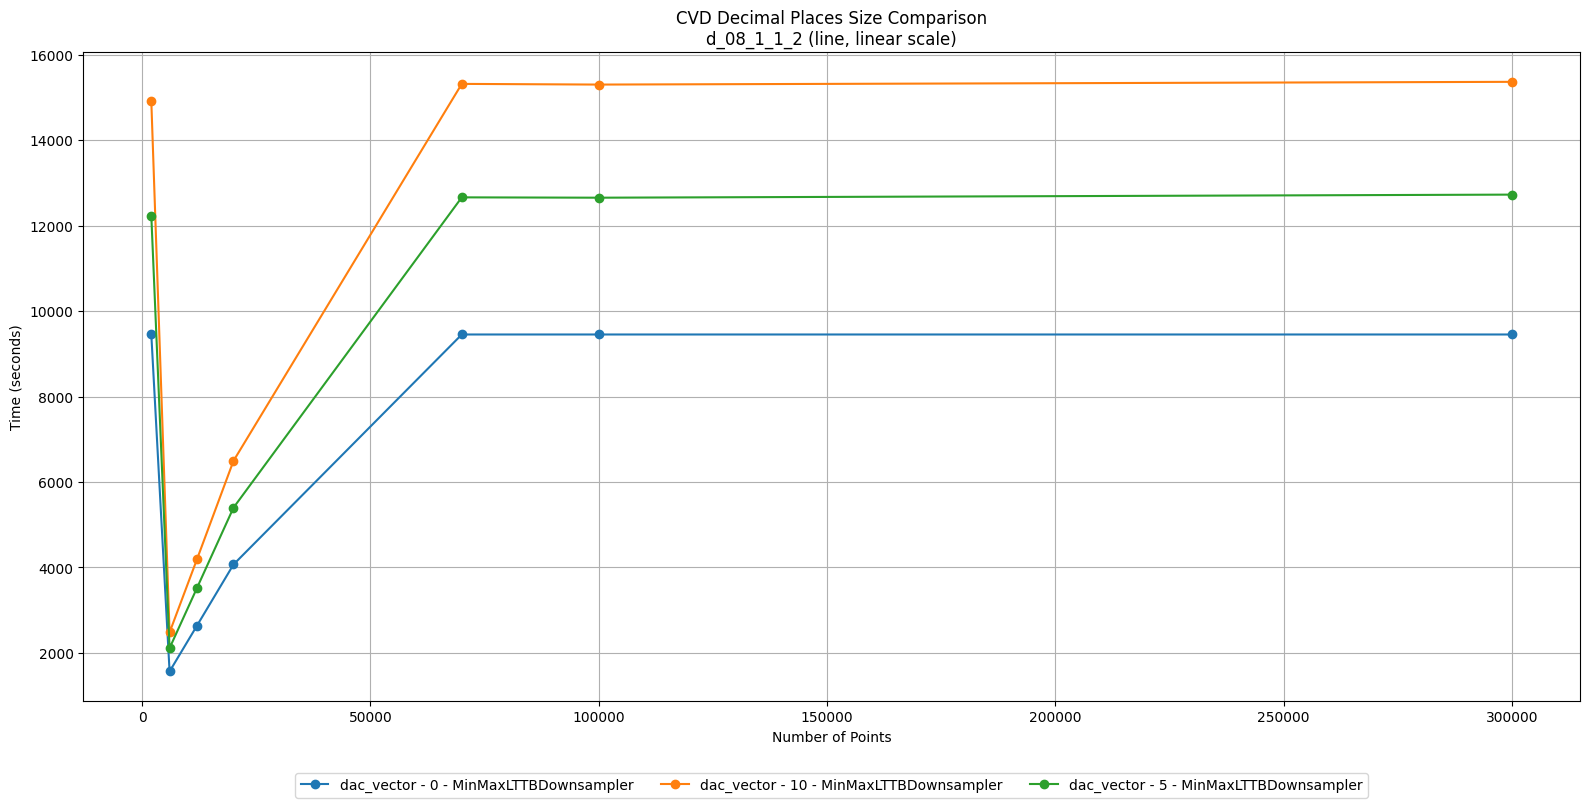
\includegraphics[width=1\textwidth]{anexo/exp/CVD Decimal Places Size Comparison/plots/CVD Decimal Places Size Comparison_d_08_1_1_2_linear_line.png}
        \caption[]{Gráfico de tamaño CVD con diferentes lugares decimales para el input \textbf{d\_08\_1\_1\_2}.}
        \label{fig:cvd_decimal_places_size_comparison_plot_line_1}
    \end{figure}
    \begin{figure}[H]
        \centering
        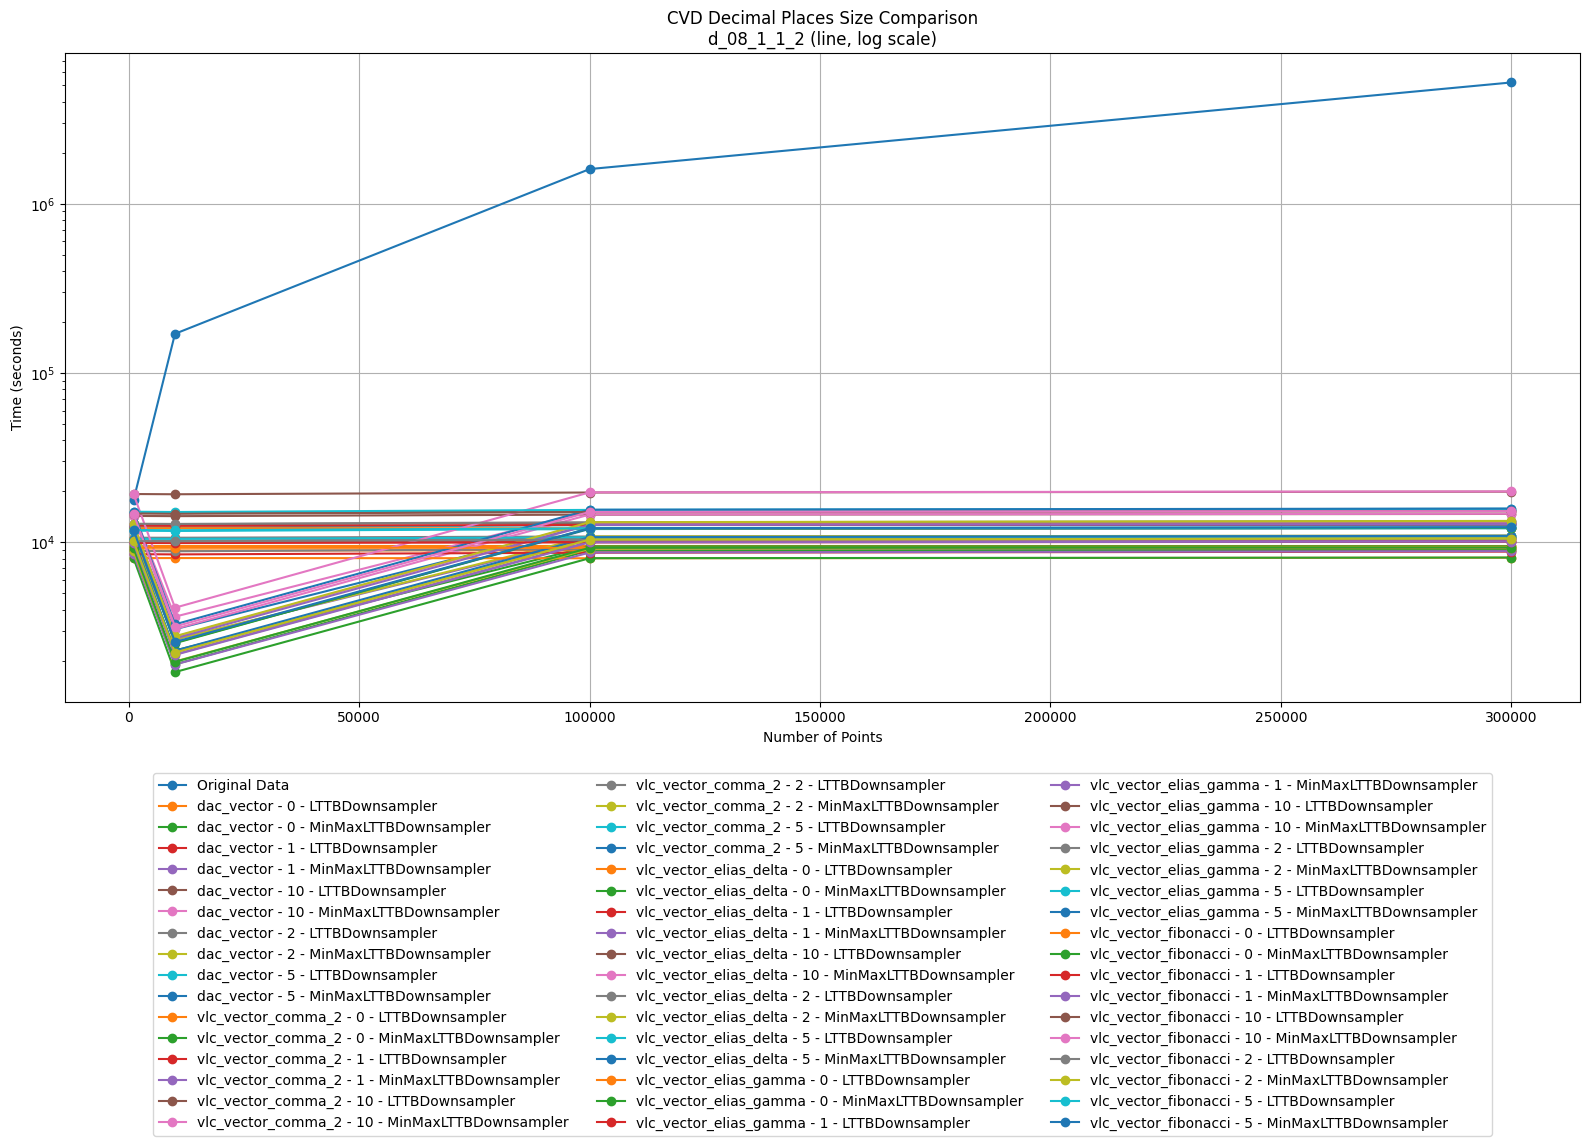
\includegraphics[width=1\textwidth]{anexo/exp/CVD Decimal Places Size Comparison/plots/CVD Decimal Places Size Comparison_d_08_1_1_2_log_line.png}
        \caption[]{Gráfico de tamaño CVD con diferentes lugares decimales para el input \textbf{d\_08\_1\_1\_2} en escala logarítmica.}
        \label{fig:cvd_decimal_places_size_comparison_plot_log_1}
    \end{figure}
}

\DeclareRobustCommand{\CVDDecimalPlacesSizeComparisonTwoPlotLine}{
    \begin{figure}[H]
        \centering
        \includegraphics[width=1\textwidth]{anexo/exp/CVD Decimal Places Size Comparison/plots/CVD Decimal Places Size Comparison_d_08_1_1_10_linear_line.png}
        \caption[]{Gráfico de tamaño CVD con diferentes lugares decimales para el input \textbf{d\_08\_1\_1\_10}.}
        \label{fig:cvd_decimal_places_size_comparison_plot_line_2}
    \end{figure}
    \begin{figure}[H]
        \centering
        \includegraphics[width=1\textwidth]{anexo/exp/CVD Decimal Places Size Comparison/plots/CVD Decimal Places Size Comparison_d_08_1_1_10_log_line.png}
        \caption[]{Gráfico de tamaño CVD con diferentes lugares decimales para el input \textbf{d\_08\_1\_1\_10} en escala logarítmica.}
        \label{fig:cvd_decimal_places_size_comparison_plot_log_2}
    \end{figure}
}

\DeclareRobustCommand{\CVDDecimalPlacesSizeComparisonThreePlotLine}{
    \begin{figure}[H]
        \centering
        \includegraphics[width=1\textwidth]{anexo/exp/CVD Decimal Places Size Comparison/plots/CVD Decimal Places Size Comparison_yellow_tripdata_2015-01_linear_line.png}
        \caption[]{Gráfico de tamaño CVD con diferentes lugares decimales para el input \textbf{yellow\_tripdata\_2015\_01}.}
        \label{fig:cvd_decimal_places_size_comparison_plot_line_3}
    \end{figure}
    \begin{figure}[H]
        \centering
        \includegraphics[width=1\textwidth]{anexo/exp/CVD Decimal Places Size Comparison/plots/CVD Decimal Places Size Comparison_yellow_tripdata_2015-01_log_line.png}
        \caption[]{Gráfico de tamaño CVD con diferentes lugares decimales para el input \textbf{yellow\_tripdata\_2015\_01} en escala logarítmica.}
        \label{fig:cvd_decimal_places_size_comparison_plot_log_3}
    \end{figure}
}





% PyGal Plotting Memory Allocation
\DeclareRobustCommand{\PyGalMemoryAllocationOnePlotLine}{
    %insertar imagen
    \begin{figure}[H]
        \centering
        \includegraphics[width=1\textwidth]{anexo/exp/Pygal Plotting Memory Allocation/plots/Pygal Plotting Memory Allocation_d_08_1_1_2_log_line.png}
        \caption[]{Gráfico de memoria asignada por PyGal para el input \textbf{d\_08\_1\_1\_2}.}
        \label{fig:pygal_memory_allocation_plot_line_1}
    \end{figure}
}

\DeclareRobustCommand{\PyGalMemoryAllocationOnePlotBar}{
    %insertar imagen
    \begin{figure}[H]
        \centering
        \includegraphics[width=1\textwidth]{anexo/exp/Pygal Plotting Memory Allocation/bar_plots/Pygal Plotting Memory Allocation_d_08_1_1_2_log_bar.png}
        \caption[]{Gráfico de memoria asignada por PyGal para el input \textbf{d\_08\_1\_1\_2}.}
        \label{fig:pygal_memory_allocation_plot_bar_1}
    \end{figure}
\begin{table}[H]
\centering
\resizebox{\textwidth}{!}{%
\begin{tabular}{|l|c|c|c|c|c|c|}
\hline\multicolumn{1}{|c|}{Option} & \multicolumn{6}{c|}{\textbf{Number of data points}} \\
\cline{2-7}
 & \textbf{6000} & \textbf{12000} & \textbf{20000} & \textbf{70000} & \textbf{100000} & \textbf{300000} \\
\hline
Compressed Vector Downsample - dac\_vector & 9.38e+02 [kb] & 1.75e+03 [kb] & 2.81e+03 [kb] & 6.88e+03 [kb] & 6.88e+03 [kb] & 6.88e+03 [kb] \\
Compressed Vector Downsample - vlc\_vector\_fibonacci & 9.38e+02 [kb] & 1.75e+03 [kb] & 2.81e+03 [kb] & 6.88e+03 [kb] & 6.88e+03 [kb] & 6.88e+03 [kb] \\
Original Data & 4.02e+04 [kb] & 8.03e+04 [kb] & 1.34e+05 [kb] & 4.70e+05 [kb] & 6.71e+05 [kb] & 2.01e+06 [kb] \\
TS Downsample & 9.37e+02 [kb] & 1.75e+03 [kb] & 2.81e+03 [kb] & 6.88e+03 [kb] & 6.88e+03 [kb] & 6.88e+03 [kb] \\
\hline
\end{tabular}
}
\label{tab:pygal plotting memory allocation-d-08-1-1-2}
\end{table}
   \begin{table}[H]
\centering
\caption{\textit{d\_08\_1\_1\_2} – Memoria por elemento}
\label{tab:d\_08\_1\_1\_2_mem_por_elemento_sin_original}
\begin{tabular}{rrrr}
\toprule
 & CVD - dac\_vector & CVD - vlc\_vector\_fibonacci & TS Downsample \\
n\_size &  &  &  \\
\midrule
6000 & 0.94 & 0.94 & 0.94 \\
12000 & 1.75 & 1.75 & 1.75 \\
20000 & 2.81 & 2.81 & 2.81 \\
70000 & 6.88 & 6.88 & 6.88 \\
100000 & 6.88 & 6.88 & 6.88 \\
300000 & 6.88 & 6.88 & 6.88 \\
\bottomrule
\end{tabular}

\end{table}
}

\DeclareRobustCommand{\PyGalMemoryAllocationTwoPlotLine}{
    %insertar imagen
    \begin{figure}[H]
        \centering
        \includegraphics[width=1\textwidth]{anexo/exp/PyGal Plotting Memory Allocation/plots/PyGal Plotting Memory Allocation_d_08_1_1_10_linear_line.png}
        \caption[]{Gráfico de memoria asignada por PyGal para el input \textbf{d\_08\_1\_1\_10}.}
        \label{fig:pygal_memory_allocation_plot_line_2}
    \end{figure}
}

\DeclareRobustCommand{\PyGalMemoryAllocationTwoPlotBar}{
    %insertar imagen
    \begin{figure}[H]
        \centering
        \includegraphics[width=1\textwidth]{anexo/exp/Pygal Plotting Memory Allocation/bar_plots/Pygal Plotting Memory Allocation_d_08_1_1_10_log_bar.png}
        \caption[]{Gráfico de memoria asignada por PyGal para el input \textbf{d\_08\_1\_1\_10}.}
        \label{fig:pygal_memory_allocation_plot_bar_2}
    \end{figure}

\begin{table}[H]
\centering
\resizebox{\textwidth}{!}{%
\begin{tabular}{|l|c|c|c|c|c|c|}
\hline\multicolumn{1}{|c|}{Option} & \multicolumn{6}{c|}{\textbf{Number of data points}} \\
\cline{2-7}
 & \textbf{6000} & \textbf{12000} & \textbf{20000} & \textbf{70000} & \textbf{100000} & \textbf{300000} \\
\hline
Compressed Vector Downsample - dac_vector & 9.36e+02 [kb] & 1.74e+03 [kb] & 2.83e+03 [kb] & 6.88e+03 [kb] & 6.88e+03 [kb] & 6.89e+03 [kb] \\
Compressed Vector Downsample - vlc_vector_fibonacci & 9.36e+02 [kb] & 1.75e+03 [kb] & 2.83e+03 [kb] & 6.88e+03 [kb] & 6.88e+03 [kb] & 6.89e+03 [kb] \\
Original Data & 4.01e+04 [kb] & 8.01e+04 [kb] & 1.33e+05 [kb] & 4.70e+05 [kb] & 6.71e+05 [kb] & 2.02e+06 [kb] \\
TS Downsample & 9.36e+02 [kb] & 1.74e+03 [kb] & 2.83e+03 [kb] & 6.88e+03 [kb] & 6.88e+03 [kb] & 6.90e+03 [kb] \\
\hline
\end{tabular}
}
\label{tab:pygal plotting memory allocation-d-08-1-1-10}
\end{table}
\begin{table}[H]
\centering
\caption{\textit{d\_08\_1\_1\_10} – Memoria por elemento}
\label{tab:d\_08\_1\_1\_10_mem_por_elemento_sin_original}
\begin{tabular}{rrrr}
\toprule
 & CVD - dac\_vector & CVD - vlc\_vector\_fibonacci & TS Downsample \\
n\_size &  &  &  \\
\midrule
6000 & 0.94 & 0.94 & 0.94 \\
12000 & 1.74 & 1.75 & 1.74 \\
20000 & 2.83 & 2.83 & 2.83 \\
70000 & 6.88 & 6.88 & 6.88 \\
100000 & 6.88 & 6.88 & 6.88 \\
300000 & 6.89 & 6.89 & 6.90 \\
\bottomrule
\end{tabular}

\end{table}
}

\DeclareRobustCommand{\PyGalMemoryAllocationThreePlotLine}{
    %insertar imagen
    \begin{figure}[H]
        \centering
        \includegraphics[width=1\textwidth]{anexo/exp/PyGal Plotting Memory Allocation/plots/PyGal Plotting Memory Allocation_yellow_tripdata_2015-01_linear_line.png}
        \caption[]{Gráfico de memoria asignada por PyGal para el input \textbf{yellow\_tripdata\_2015\_01}.}
        \label{fig:pygal_memory_allocation_plot_line_3}
    \end{figure}
}

\DeclareRobustCommand{\PyGalMemoryAllocationThreePlotBar}{
    %insertar imagen
    \begin{figure}[H]
        \centering
        \includegraphics[width=1\textwidth]{anexo/exp/Pygal Plotting Memory Allocation/bar_plots/Pygal Plotting Memory Allocation_yellow_tripdata_2015-01_log_bar.png}
        \caption[]{Gráfico de memoria asignada por PyGal para el input \textbf{yellow\_tripdata\_2015\_01}.}
        \label{fig:pygal_memory_allocation_plot_bar_3}
    \end{figure}
\begin{table}[H]
\centering
\resizebox{\textwidth}{!}{%
\begin{tabular}{|l|c|c|c|c|c|c|}
\hline\multicolumn{1}{|c|}{Option} & \multicolumn{6}{c|}{\textbf{Number of data points}} \\
\cline{2-7}
 & \textbf{6000} & \textbf{12000} & \textbf{20000} & \textbf{70000} & \textbf{100000} & \textbf{300000} \\
\hline
Compressed Vector Downsample - dac_vector & 1.33e+02 [kb] & 1.09e+02 [kb] & 1.09e+02 [kb] & 1.09e+02 [kb] & 1.53e+02 [kb] & 1.52e+02 [kb] \\
Compressed Vector Downsample - vlc_vector_fibonacci & 1.33e+02 [kb] & 1.09e+02 [kb] & 1.10e+02 [kb] & 1.09e+02 [kb] & 1.53e+02 [kb] & 1.53e+02 [kb] \\
Original Data & 4.00e+04 [kb] & 7.99e+04 [kb] & 1.33e+05 [kb] & 4.65e+05 [kb] & 6.64e+05 [kb] & 2.00e+06 [kb] \\
TS Downsample & 1.32e+02 [kb] & 1.09e+02 [kb] & 1.09e+02 [kb] & 1.08e+02 [kb] & 1.53e+02 [kb] & 1.53e+02 [kb] \\
\hline
\end{tabular}
}
\label{tab:pygal plotting memory allocation-yellow-tripdata-2015-01}
\end{table}
\begin{table}[H]
\centering
\caption{\textit{yellow\_tripdata\_2015-01} – Memoria por elemento}
\label{tab:yellow\_tripdata\_2015-01_mem_por_elemento_sin_original}
\begin{tabular}{rrrr}
\toprule
 & CVD - dac\_vector & CVD - vlc\_vector\_fibonacci & TS Downsample \\
n\_size &  &  &  \\
\midrule
6000 & 0.13 & 0.13 & 0.13 \\
12000 & 0.11 & 0.11 & 0.11 \\
20000 & 0.11 & 0.11 & 0.11 \\
70000 & 0.11 & 0.11 & 0.11 \\
100000 & 0.15 & 0.15 & 0.15 \\
300000 & 0.15 & 0.15 & 0.15 \\
\bottomrule
\end{tabular}

\end{table}
}

% PyGal Plot Time
\DeclareRobustCommand{\PyGalPlotTimeOnePlotLine}{
    %insertar imagen
    \begin{figure}[H]
        \centering
        \includegraphics[width=1\textwidth]{anexo/exp/PyGal Plot Time/plots/PyGal Plot Time_d_08_1_1_2_linear_line.png}
        \caption[]{Gráfico de tiempo de renderización PyGal para el input \textbf{d\_08\_1\_1\_2}.}
        \label{fig:pygal_plot_time_plot_line_1}
    \end{figure}
    \begin{figure}[H]
        \centering
        \includegraphics[width=1\textwidth]{anexo/exp/PyGal Plot Time/plots/PyGal Plot Time_d_08_1_1_2_log_line.png}
        \caption[]{Gráfico de tiempo de renderización PyGal para el input \textbf{d\_08\_1\_1\_2} en escala logarítmica.}
        \label{fig:pygal_plot_time_plot_line_1_log}
    \end{figure}
}

\DeclareRobustCommand{\PyGalPlotTimeOnePlotBar}{
    %insertar imagen
    \begin{figure}[H]
        \centering
        \includegraphics[width=1\textwidth]{anexo/exp/PyGal Plot Time/bar_plots/PyGal Plot Time_d_08_1_1_2_linear_bar.png}
        \caption[]{Gráfico de tiempo de renderización PyGal para el input \textbf{d\_08\_1\_1\_2}.}
        \label{fig:pygal_plot_time_plot_bar_1}
    \end{figure}
}

\DeclareRobustCommand{\PyGalPlotTimeTwoPlotLine}{
    %insertar imagen
    \begin{figure}[H]
        \centering
        \includegraphics[width=1\textwidth]{anexo/exp/PyGal Plot Time/plots/PyGal Plot Time_d_08_1_1_10_linear_line.png}
        \caption[]{Gráfico de tiempo de renderización PyGal para el input \textbf{d\_08\_1\_1\_10}.}
        \label{fig:pygal_plot_time_plot_line_2}
    \end{figure}
    \begin{figure}[H]
        \centering
        \includegraphics[width=1\textwidth]{anexo/exp/PyGal Plot Time/plots/PyGal Plot Time_d_08_1_1_10_log_line.png}
        \caption[]{Gráfico de tiempo de renderización PyGal para el input \textbf{d\_08\_1\_1\_10} en escala logarítmica.}
        \label{fig:pygal_plot_time_plot_line_2_log}
    \end{figure}
}

\DeclareRobustCommand{\PyGalPlotTimeTwoPlotBar}{
    %insertar imagen
    \begin{figure}[H]
        \centering
        \includegraphics[width=1\textwidth]{anexo/exp/PyGal Plot Time/bar_plots/PyGal Plot Time_d_08_1_1_10_linear_bar.png}
        \caption[]{Gráfico de tiempo de renderización PyGal para el input \textbf{d\_08\_1\_1\_10}.}
        \label{fig:pygal_plot_time_plot_bar_2}
    \end{figure}
}

\DeclareRobustCommand{\PyGalPlotTimeThreePlotLine}{
    %insertar imagen
    \begin{figure}[H]
        \centering
        \includegraphics[width=1\textwidth]{anexo/exp/PyGal Plot Time/plots/PyGal Plot Time_yellow_tripdata_2015-01_linear_line.png}
        \caption[]{Gráfico de tiempo de renderización PyGal para el input \textbf{yellow\_tripdata\_2015\_01}.}
        \label{fig:pygal_plot_time_plot_line_3}
    \end{figure}
    \begin{figure}[H]
        \centering
        \includegraphics[width=1\textwidth]{anexo/exp/PyGal Plot Time/plots/PyGal Plot Time_yellow_tripdata_2015-01_log_line.png}
        \caption[]{Gráfico de tiempo de renderización PyGal para el input \textbf{yellow\_tripdata\_2015\_01}.}
        \label{fig:pygal_plot_time_plot_line_3_log}
    \end{figure}
}

\DeclareRobustCommand{\PyGalPlotTimeThreePlotBar}{
    %insertar imagen
    \begin{figure}[H]
        \centering
        \includegraphics[width=1\textwidth]{anexo/exp/PyGal Plot Time/bar_plots/PyGal Plot Time_yellow_tripdata_2015-01_linear_bar.png}
        \caption[]{Gráfico de tiempo de renderización PyGal para el input \textbf{yellow\_tripdata\_2015\_01}.}
        \label{fig:pygal_plot_time_plot_bar_3}
    \end{figure}
}

\DeclareRobustCommand{\SDSLFourPyAccessTimeComparisonOnePlotBar}{
    \begin{figure}[H]
        \centering
        \includegraphics[width=1\textwidth]{anexo/exp/SDSL4Py Access Time Comparison/bar_plots/SDSL4Py Access Time Comparison_d_08_1_1_2_log_bar.png}
        \caption[]{Gráfico de tiempo de acceso SDSL4Py en escala logarítmica para el input \textbf{d\_08\_1\_1\_2}.}
        \label{fig:sdsl4py_access_time_comparison_plot_log_bar_1}
    \end{figure}
}

\DeclareRobustCommand{\SDSLFourPyAccessTimeComparisonTwoPlotBar}{
    \begin{figure}[H]
        \centering
        \includegraphics[width=1\textwidth]{anexo/exp/SDSL4Py Access Time Comparison/bar_plots/SDSL4Py Access Time Comparison_d_08_1_1_10_log_bar.png}
        \caption[]{Gráfico de tiempo de acceso SDSL4Py en escala logarítmica para el input \textbf{d\_08\_1\_1\_10}.}
        \label{fig:sdsl4py_access_time_comparison_plot_log_bar_2}
    \end{figure}
}

\DeclareRobustCommand{\SDSLFourPyAccessTimeComparisonThreePlotBar}{
    \begin{figure}[H]
        \centering
        \includegraphics[width=1\textwidth]{anexo/exp/SDSL4Py Access Time Comparison/bar_plots/SDSL4Py Access Time Comparison_yellow_tripdata_2015-01_log_bar.png}
        \caption[]{Gráfico de tiempo de acceso SDSL4Py en escala logarítmica para el input \textbf{yellow\_tripdata\_2015\_01}.}
        \label{fig:sdsl4py_access_time_comparison_plot_log_bar_3}
    \end{figure}
}

\DeclareRobustCommand{\SDSLFourPyCompressionSpaceComparisonOnePlotBar}{
    \begin{figure}[H]
        \centering
        \includegraphics[width=1\textwidth]{anexo/exp/SDSL4Py Compression Space Comparison/bar_plots/SDSL4Py Compression Space Comparison_d_08_1_1_2_log_bar.png}
        \caption[]{Gráfico de espacio de compresión SDSL4Py en escala logarítmica para el input \textbf{d\_08\_1\_1\_2}.}
        \label{fig:sdsl4py_compression_space_comparison_plot_log_bar_1}
    \end{figure}
}

\DeclareRobustCommand{\SDSLFourPyCompressionSpaceComparisonTwoPlotBar}{
    \begin{figure}[H]
        \centering
        \includegraphics[width=1\textwidth]{anexo/exp/SDSL4Py Compression Space Comparison/bar_plots/SDSL4Py Compression Space Comparison_d_08_1_1_10_log_bar.png}
        \caption[]{Gráfico de espacio de compresión SDSL4Py en escala logarítmica para el input \textbf{d\_08\_1\_1\_10}.}
        \label{fig:sdsl4py_compression_space_comparison_plot_log_bar_2}
    \end{figure}
}

\DeclareRobustCommand{\SDSLFourPyCompressionSpaceComparisonThreePlotBar}{
    \begin{figure}[H]
        \centering
        \includegraphics[width=1\textwidth]{anexo/exp/SDSL4Py Compression Space Comparison/bar_plots/SDSL4Py Compression Space Comparison_yellow_tripdata_2015-01_log_bar.png}
        \caption[]{Gráfico de espacio de compresión SDSL4Py en escala logarítmica para el input \textbf{yellow\_tripdata\_2015\_01}.}
        \label{fig:sdsl4py_compression_space_comparison_plot_log_bar_3}
    \end{figure}
}
\DeclareRobustCommand{\SDSLFourPyCompressionTimeComparisonOnePlotBar}{
    \begin{figure}[H]
        \centering
        \includegraphics[width=1\textwidth]{anexo/exp/SDSL4Py Compression Time Comparison/bar_plots/SDSL4Py Compression Time Comparison_d_08_1_1_2_log_bar.png}
        \caption[]{Gráfico de tiempo de compresión SDSL4Py en escala logarítmica para el input \textbf{d\_08\_1\_1\_2}.}
        \label{fig:sdsl4py_compression_time_comparison_plot_log_bar_1}
    \end{figure}
}

\DeclareRobustCommand{\SDSLFourPyCompressionTimeComparisonTwoPlotBar}{
    \begin{figure}[H]
        \centering
        \includegraphics[width=1\textwidth]{anexo/exp/SDSL4Py Compression Time Comparison/bar_plots/SDSL4Py Compression Time Comparison_d_08_1_1_10_log_bar.png}
        \caption[]{Gráfico de tiempo de compresión SDSL4Py en escala logarítmica para el input \textbf{d\_08\_1\_1\_10}.}
        \label{fig:sdsl4py_compression_time_comparison_plot_log_bar_2}
    \end{figure}
}

\DeclareRobustCommand{\SDSLFourPyCompressionTimeComparisonThreePlotBar}{
    \begin{figure}[H]
        \centering
        \includegraphics[width=1\textwidth]{anexo/exp/SDSL4Py Compression Time Comparison/bar_plots/SDSL4Py Compression Time Comparison_yellow_tripdata_2015-01_log_bar.png}
        \caption[]{Gráfico de tiempo de compresión SDSL4Py en escala logarítmica para el input \textbf{yellow\_tripdata\_2015\_01}.}
        \label{fig:sdsl4py_compression_time_comparison_plot_log_bar_3}
    \end{figure}
}


% Vega-Altair Plot Time Comparison
\DeclareRobustCommand{\VegaAltairPlotTimeComparisonOnePlotLine}{
    %insertar imagen
    \begin{figure}[H]
        \centering
        \includegraphics[width=1\textwidth]{anexo/exp/Vega-Altair Plot Time Comparison/plots/Vega-Altair Plot Time Comparison_d_08_1_1_2_linear_line.png}
        \caption[]{Gráfico de tiempo de renderización Vega-Altair para el input \textbf{d\_08\_1\_1\_2}.}
        \label{fig:vega_altair_plot_time_comparison_plot_line_1}
    \end{figure}
    \begin{figure}[H]
        \centering
        \includegraphics[width=1\textwidth]{anexo/exp/Vega-Altair Plot Time Comparison/plots/Vega-Altair Plot Time Comparison_d_08_1_1_2_log_line.png}
        \caption[]{Gráfico de tiempo de renderización Vega-Altair para el input \textbf{d\_08\_1\_1\_2} en escala logarítmica.}
        \label{fig:vega_altair_plot_time_comparison_plot_line_1}
    \end{figure}
}

\DeclareRobustCommand{\VegaAltairPlotTimeComparisonOnePlotBar}{
    %insertar imagen
    \begin{figure}[H]
        \centering
        \includegraphics[width=1\textwidth]{anexo/exp/Vega-Altair Plot Time Comparison/bar_plots/Vega-Altair Plot Time Comparison_d_08_1_1_2_linear_bar.png}
        \caption[]{Gráfico de tiempo de renderización Vega-Altair para el input \textbf{d\_08\_1\_1\_2}.}
        \label{fig:vega_altair_plot_time_comparison_plot_bar_1}
    \end{figure}
}

\DeclareRobustCommand{\VegaAltairPlotTimeComparisonTwoPlotLine}{
    %insertar imagen
    \begin{figure}[H]
        \centering
        \includegraphics[width=1\textwidth]{anexo/exp/Vega-Altair Plot Time Comparison/plots/Vega-Altair Plot Time Comparison_d_08_1_1_10_linear_line.png}
        \caption[]{Gráfico de tiempo de renderización Vega-Altair para el input \textbf{d\_08\_1\_1\_10}.}
        \label{fig:vega_altair_plot_time_comparison_plot_line_2}
    \end{figure}
}

\DeclareRobustCommand{\VegaAltairPlotTimeComparisonTwoPlotBar}{
    %insertar imagen
    \begin{figure}[H]
        \centering
        \includegraphics[width=1\textwidth]{anexo/exp/Vega-Altair Plot Time Comparison/bar_plots/Vega-Altair Plot Time Comparison_d_08_1_1_10_linear_bar.png}
        \caption[]{Gráfico de tiempo de renderización Vega-Altair para el input \textbf{d\_08\_1\_1\_10}.}
        \label{fig:vega_altair_plot_time_comparison_plot_bar_2}
    \end{figure}
}

\DeclareRobustCommand{\VegaAltairPlotTimeComparisonThreePlotLine}{
    %insertar imagen
    \begin{figure}[H]
        \centering
        \includegraphics[width=1\textwidth]{anexo/exp/Vega-Altair Plot Time Comparison/plots/Vega-Altair Plot Time Comparison_yellow_tripdata_2015-01_linear_line.png}
        \caption[]{Gráfico de tiempo de renderización Vega-Altair para el input \textbf{yellow\_tripdata\_2015\_01}.}
        \label{fig:vega_altair_plot_time_comparison_plot_line_3}
    \end{figure}
}

\DeclareRobustCommand{\VegaAltairPlotTimeComparisonThreePlotBar}{
    %insertar imagen
    \begin{figure}[H]
        \centering
        \includegraphics[width=1\textwidth]{anexo/exp/Vega-Altair Plot Time Comparison/bar_plots/Vega-Altair Plot Time Comparison_yellow_tripdata_2015-01_linear_bar.png}
        \caption[]{Gráfico de tiempo de renderización Vega-Altair para el input \textbf{yellow\_tripdata\_2015\_01}.}
        \label{fig:vega_altair_plot_time_comparison_plot_bar_3}
    \end{figure}
}

% Vega-Altair Plotting + Building Comparison
\DeclareRobustCommand{\VegaAltairPlottingBuildingComparisonOnePlotLine}{
    %insertar imagen
    \begin{figure}[H]
        \centering
        \includegraphics[width=1\textwidth]{anexo/exp/Vega-Altair Plotting + Building Comparison/plots/Vega-Altair Plotting + Building Comparison_d_08_1_1_2_linear_line.png}
        \caption[]{Gráfico de tiempo de renderización y construcción Vega-Altair para el input \textbf{d\_08\_1\_1\_2}.}
        \label{fig:vega_altair_plotting_building_comparison_plot_line_1}
    \end{figure}
}

\DeclareRobustCommand{\VegaAltairPlottingBuildingComparisonOnePlotBar}{
    %insertar imagen
    \begin{figure}[H]
        \centering
        \includegraphics[width=1\textwidth]{anexo/exp/Vega-Altair Plotting + Building Comparison/bar_plots/Vega-Altair Plotting + Building Comparison_d_08_1_1_2_linear_bar.png}
        \caption[]{Gráfico de tiempo de renderización y construcción Vega-Altair para el input \textbf{d\_08\_1\_1\_2}.}
        \label{fig:vega_altair_plotting_building_comparison_plot_bar_1}
    \end{figure}
}

\DeclareRobustCommand{\VegaAltairPlottingBuildingComparisonTwoPlotLine}{
    %insertar imagen
    \begin{figure}[H]
        \centering
        \includegraphics[width=1\textwidth]{anexo/exp/Vega-Altair Plotting + Building Comparison/plots/Vega-Altair Plotting + Building Comparison_d_08_1_1_10_linear_line.png}
        \caption[]{Gráfico de tiempo de renderización y construcción Vega-Altair para el input \textbf{d\_08\_1\_1\_10}.}
        \label{fig:vega_altair_plotting_building_comparison_plot_line_2}
    \end{figure}
}

\DeclareRobustCommand{\VegaAltairPlottingBuildingComparisonTwoPlotBar}{
    %insertar imagen
    \begin{figure}[H]
        \centering
        \includegraphics[width=1\textwidth]{anexo/exp/Vega-Altair Plotting + Building Comparison/bar_plots/Vega-Altair Plotting + Building Comparison_d_08_1_1_10_linear_bar.png}
        \caption[]{Gráfico de tiempo de renderización y construcción Vega-Altair para el input \textbf{d\_08\_1\_1\_10}.}
        \label{fig:vega_altair_plotting_building_comparison_plot_bar_2}
    \end{figure}
}

\DeclareRobustCommand{\VegaAltairPlottingBuildingComparisonThreePlotLine}{
    %insertar imagen
    \begin{figure}[H]
        \centering
        \includegraphics[width=1\textwidth]{anexo/exp/Vega-Altair Plotting + Building Comparison/plots/Vega-Altair Plotting + Building Comparison_yellow_tripdata_2015-01_linear_line.png}
        \caption[]{Gráfico de tiempo de renderización y construcción Vega-Altair para el input \textbf{yellow\_tripdata\_2015\_01}.}
        \label{fig:vega_altair_plotting_building_comparison_plot_line_3}
    \end{figure}
}

\DeclareRobustCommand{\VegaAltairPlottingBuildingComparisonThreePlotBar}{
    %insertar imagen
    \begin{figure}[H]
        \centering
        \includegraphics[width=1\textwidth]{anexo/exp/Vega-Altair Plotting + Building Comparison/bar_plots/Vega-Altair Plotting + Building Comparison_yellow_tripdata_2015-01_linear_bar.png}
        \caption[]{Gráfico de tiempo de renderización y construcción Vega-Altair para el input \textbf{yellow\_tripdata\_2015\_01}.}
        \label{fig:vega_altair_plotting_building_comparison_plot_bar_3}
    \end{figure}
}

% VEGA ALTAIR MEMORY ALLOCATION

\DeclareRobustCommand{\VegaAltairMemoryAllocationOnePlotLine}{
    %insertar imagen
    \begin{figure}[H]
        \centering
        \includegraphics[width=1\textwidth]{anexo/exp/Vega-Altair Plotting Memory Allocation/plots/Vega-Altair Plotting Memory Allocation_d_08_1_1_2_log_line.png}
        \caption[]{Gráfico de tiempo de renderización y construcción Vega-Altair para el input \textbf{d\_08\_1\_1\_2}.}
        \label{fig:vega_altair_plotting_building_comparison_plot_line_1}
    \end{figure}
}

\DeclareRobustCommand{\VegaAltairMemoryAllocationOnePlotBar}{
    %insertar imagen
    \begin{figure}[H]
        \centering
        \includegraphics[width=1\textwidth]{anexo/exp/Vega-Altair Plotting Memory Allocation/bar_plots/Vega-Altair Plotting Memory Allocation_d_08_1_1_2_log_bar.png}
        \caption[]{Gráfico de tiempo de renderización y construcción Vega-Altair para el input \textbf{d\_08\_1\_1\_2}.}
        \label{fig:vega_altair_plotting_building_comparison_plot_bar_1}
    \end{figure}
\begin{table}[H]
\centering
\caption{\textit{d\_08\_1\_1\_2} – Memoria por elemento [KB]}
\label{tab:Vega-Altair Plotting Memory Allocation\_d\_08\_1\_1\_2_mem_por_elemento_sin_original}
\begin{tabular}{rrrr}
\toprule
 & CVD - dac\_vector & CVD - vlc\_vector\_fibonacci & TS Downsample \\
n\_size &  &  &  \\
\midrule
6000 & 0.16 & 0.16 & 0.16 \\
12000 & 0.16 & 0.16 & 0.16 \\
20000 & 0.17 & 0.17 & 0.16 \\
70000 & 0.18 & 0.18 & 0.17 \\
100000 & 0.18 & 0.18 & 0.17 \\
300000 & 0.19 & 0.18 & 0.17 \\
\bottomrule
\end{tabular}

\end{table}
}

\DeclareRobustCommand{\VegaAltairMemoryAllocationTwoPlotLine}{
    %insertar imagen
    \begin{figure}[H]
        \centering
        \includegraphics[width=1\textwidth]{anexo/exp/Vega-Altair Plotting Memory Allocation/plots/Vega-Altair Plotting Memory Allocation_d_08_1_1_10_log_line.png}
        \caption[]{Gráfico de tiempo de renderización y construcción Vega-Altair para el input \textbf{d\_08\_1\_1\_10}.}
        \label{fig:vega_altair_plotting_building_comparison_plot_line_2}
    \end{figure}
}

\DeclareRobustCommand{\VegaAltairMemoryAllocationTwoPlotBar}{
    %insertar imagen
    \begin{figure}[H]
        \centering
        \includegraphics[width=1\textwidth]{anexo/exp/Vega-Altair Plotting Memory Allocation/bar_plots/Vega-Altair Plotting Memory Allocation_d_08_1_1_10_log_bar.png}
        \caption[]{Gráfico de asignación de memoria con la biblioteca Vega-Altair para el input \textbf{d\_08\_1\_1\_10}.}
        \label{fig:vega_altair_plotting_building_comparison_plot_bar_2}
    \end{figure}
\begin{table}[H]
\centering
\caption{\textit{d\_08\_1\_1\_10} – Memoria por elemento [KB]}
\label{tab:Vega-Altair Plotting Memory Allocation\_d\_08\_1\_1\_10_mem_por_elemento_sin_original}
\begin{tabular}{rrrr}
\toprule
 & CVD - dac\_vector & CVD - vlc\_vector\_fibonacci & TS Downsample \\
n\_size &  &  &  \\
\midrule
6000 & 0.16 & 0.16 & 0.16 \\
12000 & 0.16 & 0.16 & 0.16 \\
20000 & 0.17 & 0.17 & 0.16 \\
70000 & 0.18 & 0.18 & 0.17 \\
100000 & 0.18 & 0.18 & 0.17 \\
300000 & 0.18 & 0.20 & 0.17 \\
\bottomrule
\end{tabular}

\end{table}
}

\DeclareRobustCommand{\VegaAltairMemoryAllocationThreePlotLine}{
    %insertar imagen
    \begin{figure}[H]
        \centering
        \includegraphics[width=1\textwidth]{anexo/exp/Vega-Altair Plotting Memory Allocation/plots/Vega-Altair Plotting Memory Allocation_yellow_tripdata_2015-01_log_line.png}
        \caption[]{Gráfico de asignación de memoria con la biblioteca Vega-Altair para el input \textbf{yellow\_tripdata\_2015\_01}.}
        \label{fig:vega_altair_plotting_building_comparison_plot_line_3}
    \end{figure}
}

\DeclareRobustCommand{\VegaAltairMemoryAllocationThreePlotBar}{
    %insertar imagen
    \begin{figure}[H]
        \centering
        \includegraphics[width=1\textwidth]{anexo/exp/Vega-Altair Plotting Memory Allocation/bar_plots/Vega-Altair Plotting Memory Allocation_yellow_tripdata_2015-01_log_bar.png}
        \caption[]{Gráfico de asignación de memoria con la biblioteca Vega-Altair para el input \textbf{yellow\_tripdata\_2015\_01}.}
        \label{fig:vega_altair_plotting_building_comparison_plot_bar_3}
    \end{figure}
\begin{table}[H]
\centering
\caption{\textit{yellow\_tripdata\_2015-01} – Memoria por elemento [KB]}
\label{tab:Vega-Altair Plotting Memory Allocation\_yellow\_tripdata\_2015-01_mem_por_elemento_sin_original}
\begin{tabular}{rrrr}
\toprule
 & CVD - dac\_vector & CVD - vlc\_vector\_fibonacci & TS Downsample \\
n\_size &  &  &  \\
\midrule
6000 & 0.16 & 0.16 & 0.16 \\
12000 & 0.16 & 0.16 & 0.16 \\
20000 & 0.16 & 0.16 & 0.16 \\
70000 & 0.16 & 0.16 & 0.16 \\
100000 & 0.16 & 0.16 & 0.16 \\
300000 & 0.16 & 0.16 & 0.16 \\
\bottomrule
\end{tabular}

\end{table}
}

% All Libraries Memory Allocation

\DeclareRobustCommand{\AllLibrariesMemoryAllocationOneTable}
{
    \vspace{0.5em}
    \input{anexo/exp/All Libraries Memory Allocation/txts/All Libraries Memory Allocation_d_08_1_1_2.txt}
}
\DeclareRobustCommand{\AllLibrariesMemoryAllocationTwoTable}
{
    \vspace{0.5em}
    \input{anexo/exp/All Libraries Memory Allocation/txts/All Libraries Memory Allocation_d_08_1_1_2_10.txt}
}
\DeclareRobustCommand{\AllLibrariesMemoryAllocationThreeTable}
{
    \vspace{0.5em}
    \input{anexo/exp/All Libraries Memory Allocation/txts/All Libraries Memory Allocation_yellow_tripdata_2015-01.txt}
}

% All Libraries Time Comparison
\DeclareRobustCommand{\AllLibrariesTimeComparisonOneTable}
{
    \vspace{0.5em}
    \input{anexo/exp/All Libraries Time Comparison/txts/All Libraries Time Comparison_d_08_1_1_2.txt}
}
\DeclareRobustCommand{\AllLibrariesTimeComparisonTwoTable}
{
    \vspace{0.5em}
    \input{anexo/exp/All Libraries Time Comparison/txts/All Libraries Time Comparison_d_08_1_1_2_10.txt}
}
\DeclareRobustCommand{\AllLibrariesTimeComparisonThreeTable}
{
    \vspace{0.5em}
    \input{anexo/exp/All Libraries Time Comparison/txts/All Libraries Time Comparison_yellow_tripdata_2015-01.txt}
}

% Building Time Comparison
\DeclareRobustCommand{\BuildingTimeComparisonOneTable}
{
    \vspace{0.5em}
    \input{anexo/exp/Building Time Comparison/txts/Building Time Comparison_d_08_1_1_2.txt}
}
\DeclareRobustCommand{\BuildingTimeComparisonTwoTable}
{
    \vspace{0.5em}
    \input{anexo/exp/Building Time Comparison/txts/Building Time Comparison_d_08_1_1_2_10.txt}
}
\DeclareRobustCommand{\BuildingTimeComparisonThreeTable}
{
    \vspace{0.5em}
    \input{anexo/exp/Building Time Comparison/txts/Building Time Comparison_yellow_tripdata_2015-01.txt}
}

% Comparison of Space Used
\DeclareRobustCommand{\ComparisonOfSpaceUsedOneTable}
{
    \vspace{0.5em}
    \input{anexo/exp/Comparison of Space Used/txts/Comparison of Space Used_d_08_1_1_2.txt}
}
\DeclareRobustCommand{\ComparisonOfSpaceUsedTwoTable}
{
    \vspace{0.5em}
    \input{anexo/exp/Comparison of Space Used/txts/Comparison of Space Used_d_08_1_1_2_10.txt}
}
\DeclareRobustCommand{\ComparisonOfSpaceUsedThreeTable}
{
    \vspace{0.5em}
    \input{anexo/exp/Comparison of Space Used/txts/Comparison of Space Used_yellow_tripdata_2015-01.txt}
}

% CVD Decimal Places Access Time Comparison
\DeclareRobustCommand{\CVDDecimalPlacesAccessTimeComparisonOneTable}
{
    \vspace{0.5em}
    \input{anexo/exp/CVD Decimal Places Access Time Comparison/txts/CVD Decimal Places Access Time Comparison_d_08_1_1_2.txt}
}
\DeclareRobustCommand{\CVDDecimalPlacesAccessTimeComparisonTwoTable}
{
    \vspace{0.5em}
    \input{anexo/exp/CVD Decimal Places Access Time Comparison/txts/CVD Decimal Places Access Time Comparison_d_08_1_1_10.txt}
}
\DeclareRobustCommand{\CVDDecimalPlacesAccessTimeComparisonThreeTable}
{
    \vspace{0.5em}
    \input{anexo/exp/CVD Decimal Places Access Time Comparison/txts/CVD Decimal Places Access Time Comparison_yellow_tripdata_2015-01.txt}
}

% CVD Decimal Places Build Time Comparison
\DeclareRobustCommand{\CVDDecimalPlacesBuildTimeComparisonOneTable}
{
    \vspace{0.5em}
    \input{anexo/exp/CVD Decimal Places Build Time Comparison/txts/CVD Decimal Places Build Time Comparison_d_08_1_1_2.txt}
}
\DeclareRobustCommand{\CVDDecimalPlacesBuildTimeComparisonTwoTable}
{
    \vspace{0.5em}
    \input{anexo/exp/CVD Decimal Places Build Time Comparison/txts/CVD Decimal Places Build Time Comparison_d_08_1_1_10.txt}
}
\DeclareRobustCommand{\CVDDecimalPlacesBuildTimeComparisonThreeTable}
{
    \vspace{0.5em}
    \input{anexo/exp/CVD Decimal Places Build Time Comparison/txts/CVD Decimal Places Build Time Comparison_yellow_tripdata_2015-01.txt}
}

% CVD Decimal Places Size Comparison
\DeclareRobustCommand{\CVDDecimalPlacesSizeComparisonOneTable}
{
    \vspace{0.5em}
    \input{anexo/exp/CVD Decimal Places Size Comparison/txts/CVD Decimal Places Size Comparison_d_08_1_1_2.txt}
}
\DeclareRobustCommand{\CVDDecimalPlacesSizeComparisonTwoTable}
{
    \vspace{0.5em}
    \input{anexo/exp/CVD Decimal Places Size Comparison/txts/CVD Decimal Places Size Comparison_d_08_1_1_10.txt}
}
\DeclareRobustCommand{\CVDDecimalPlacesSizeComparisonThreeTable}
{
    \vspace{0.5em}
    \input{anexo/exp/CVD Decimal Places Size Comparison/txts/CVD Decimal Places Size Comparison_yellow_tripdata_2015-01.txt}
}

% PyGal Memory Allocation
\DeclareRobustCommand{\PyGalMemoryAllocationOneTable}
{
    \vspace{0.5em}
    \input{anexo/exp/PyGal Memory Allocation/txts/PyGal Memory Allocation_d_08_1_1_2.txt}
}
\DeclareRobustCommand{\PyGalMemoryAllocationTwoTable}
{
    \vspace{0.5em}
    \input{anexo/exp/PyGal Memory Allocation/txts/PyGal Memory Allocation_d_08_1_1_10.txt}
}
\DeclareRobustCommand{\PyGalMemoryAllocationThreeTable}
{
    \vspace{0.5em}
    \input{anexo/exp/PyGal Memory Allocation/txts/PyGal Memory Allocation_yellow_tripdata_2015-01.txt}
}

% PyGal Plot Time
\DeclareRobustCommand{\PyGalPlotTimeOneTable}
{
    \vspace{0.5em}
    \input{anexo/exp/PyGal Plot Time/txts/PyGal Plot Time_d_08_1_1_2.txt}
}
\DeclareRobustCommand{\PyGalPlotTimeTwoTable}
{
    \vspace{0.5em}
    \input{anexo/exp/PyGal Plot Time/txts/PyGal Plot Time_d_08_1_1_10.txt}
}
\DeclareRobustCommand{\PyGalPlotTimeThreeTable}
{
    \vspace{0.5em}
    \input{anexo/exp/PyGal Plot Time/txts/PyGal Plot Time_yellow_tripdata_2015-01.txt}
}

% SDSL4Py Access Time Comparison
\DeclareRobustCommand{\SDSLFourPyAccessTimeComparisonOneTable}
{
    \vspace{0.5em}
    \input{anexo/exp/SDSL4Py Access Time Comparison/txts/SDSL4Py Access Time Comparison_d_08_1_1_2.txt}
}
\DeclareRobustCommand{\SDSLFourPyAccessTimeComparisonTwoTable}
{
    \vspace{0.5em}
    \input{anexo/exp/SDSL4Py Access Time Comparison/txts/SDSL4Py Access Time Comparison_d_08_1_1_10.txt}
}
\DeclareRobustCommand{\SDSLFourPyAccessTimeComparisonThreeTable}
{
    \vspace{0.5em}
    \input{anexo/exp/SDSL4Py Access Time Comparison/txts/SDSL4Py Access Time Comparison_yellow_tripdata_2015-01.txt}
}

% SDSL4Py Compression Space Comparison
\DeclareRobustCommand{\SDSLFourPyCompressionSpaceComparisonOneTable}
{
    \vspace{0.5em}
    \input{anexo/exp/SDSL4Py Compression Space Comparison/txts/SDSL4Py Compression Space Comparison_d_08_1_1_2.txt}
}
\DeclareRobustCommand{\SDSLFourPyCompressionSpaceComparisonTwoTable}
{
    \vspace{0.5em}
    \input{anexo/exp/SDSL4Py Compression Space Comparison/txts/SDSL4Py Compression Space Comparison_d_08_1_1_10.txt}
}
\DeclareRobustCommand{\SDSLFourPyCompressionSpaceComparisonThreeTable}
{
    \vspace{0.5em}
    \input{anexo/exp/SDSL4Py Compression Space Comparison/txts/SDSL4Py Compression Space Comparison_yellow_tripdata_2015-01.txt}
}

% SDSL4Py Compression Time Comparison
\DeclareRobustCommand{\SDSLFourPyCompressionTimeComparisonOneTable}
{
    \vspace{0.5em}
    \input{anexo/exp/SDSL4Py Compression Time Comparison/txts/SDSL4Py Compression Time Comparison_d_08_1_1_2.txt}
}
\DeclareRobustCommand{\SDSLFourPyCompressionTimeComparisonTwoTable}
{
    \vspace{0.5em}
    \input{anexo/exp/SDSL4Py Compression Time Comparison/txts/SDSL4Py Compression Time Comparison_d_08_1_1_10.txt}
}
\DeclareRobustCommand{\SDSLFourPyCompressionTimeComparisonThreeTable}
{
    \vspace{0.5em}
    \input{anexo/exp/SDSL4Py Compression Time Comparison/txts/SDSL4Py Compression Time Comparison_yellow_tripdata_2015-01.txt}
}

% Vega-Altair Plot Time Comparison
\DeclareRobustCommand{\VegaAltairPlotTimeComparisonOneTable}
{
    \vspace{0.5em}
    \input{anexo/exp/Vega-Altair Plot Time Comparison/txts/Vega-Altair Plot Time Comparison_d_08_1_1_2.txt}
}
\DeclareRobustCommand{\VegaAltairPlotTimeComparisonTwoTable}
{
    \vspace{0.5em}
    \input{anexo/exp/Vega-Altair Plot Time Comparison/txts/Vega-Altair Plot Time Comparison_d_08_1_1_10.txt}
}
\DeclareRobustCommand{\VegaAltairPlotTimeComparisonThreeTable}
{
    \vspace{0.5em}
    \input{anexo/exp/Vega-Altair Plot Time Comparison/txts/Vega-Altair Plot Time Comparison_yellow_tripdata_2015-01.txt}
}

% Vega-Altair Plotting + Building Comparison
\DeclareRobustCommand{\VegaAltairPlottingBuildingComparisonOneTable}
{
    \vspace{0.5em}
    \input{anexo/exp/Vega-Altair Plotting + Building Comparison/txts/Vega-Altair Plotting + Building Comparison_d_08_1_1_2.txt}
}
\DeclareRobustCommand{\VegaAltairPlottingBuildingComparisonTwoTable}
{
    \vspace{0.5em}
    \input{anexo/exp/Vega-Altair Plotting + Building Comparison/txts/Vega-Altair Plotting + Building Comparison_d_08_1_1_10.txt}
}
\DeclareRobustCommand{\VegaAltairPlottingBuildingComparisonThreeTable}
{
    \vspace{0.5em}
    \input{anexo/exp/Vega-Altair Plotting + Building Comparison/txts/Vega-Altair Plotting + Building Comparison_yellow_tripdata_2015-01.txt}
}

\DeclareRobustCommand{\AllLibrariesMemoryAllocation}
{
    \AllLibrariesMemoryAllocationOnePlotBar
    \AllLibrariesMemoryAllocationOnePlotLine
    \AllLibrariesMemoryAllocationOneTable

    \AllLibrariesMemoryAllocationTwoPlotBar
    \AllLibrariesMemoryAllocationTwoPlotLine
    \AllLibrariesMemoryAllocationTwoTable

    \AllLibrariesMemoryAllocationThreePlotBar
    \AllLibrariesMemoryAllocationThreePlotLine
    \AllLibrariesMemoryAllocationThreeTable
}

\DeclareRobustCommand{\AllLibrariesTimeComparison}
{
    \AllLibrariesTimeComparisonOnePlotBar
    \AllLibrariesTimeComparisonOnePlotLine
    \AllLibrariesTimeComparisonOneTable

    \AllLibrariesTimeComparisonTwoPlotBar
    \AllLibrariesTimeComparisonTwoPlotLine
    \AllLibrariesTimeComparisonTwoTable
    
    \AllLibrariesTimeComparisonThreePlotBar
    \AllLibrariesTimeComparisonThreePlotLine
    \AllLibrariesTimeComparisonThreeTable
}

\DeclareRobustCommand{\BuildingTimeComparison}
{
    \BuildingTimeComparisonOnePlotBar
    \BuildingTimeComparisonOnePlotLine
    \BuildingTimeComparisonOneTable

    \BuildingTimeComparisonTwoPlotBar
    \BuildingTimeComparisonTwoPlotLine
    \BuildingTimeComparisonTwoTable
    
    \BuildingTimeComparisonThreePlotBar
    \BuildingTimeComparisonThreePlotLine
    \BuildingTimeComparisonThreeTable
}

\DeclareRobustCommand{\ComparisonOfSpaceUsed}
{
    \ComparisonOfSpaceUsedOnePlotBar
    \ComparisonOfSpaceUsedOnePlotLine
    \ComparisonOfSpaceUsedOneTable

    \ComparisonOfSpaceUsedTwoPlotBar
    \ComparisonOfSpaceUsedTwoPlotLine
    \ComparisonOfSpaceUsedTwoTable
    
    \ComparisonOfSpaceUsedThreePlotBar
    \ComparisonOfSpaceUsedThreePlotLine
    \ComparisonOfSpaceUsedThreeTable
}

\DeclareRobustCommand{\CVDDecimalPlacesAccessTimeComparison}
{
    \CVDDecimalPlacesAccessTimeComparisonOnePlotBar
    \CVDDecimalPlacesAccessTimeComparisonOnePlotLine
    \CVDDecimalPlacesAccessTimeComparisonOneTable

    \CVDDecimalPlacesAccessTimeComparisonTwoPlotBar
    \CVDDecimalPlacesAccessTimeComparisonTwoPlotLine
    \CVDDecimalPlacesAccessTimeComparisonTwoTable
    
    \CVDDecimalPlacesAccessTimeComparisonThreePlotBar
    \CVDDecimalPlacesAccessTimeComparisonThreePlotLine
    \CVDDecimalPlacesAccessTimeComparisonThreeTable
}

\DeclareRobustCommand{\CVDDecimalPlacesBuildTimeComparison}
{
    \CVDDecimalPlacesBuildTimeComparisonOnePlotBar
    \CVDDecimalPlacesBuildTimeComparisonOnePlotLine
    \CVDDecimalPlacesBuildTimeComparisonOneTable

    \CVDDecimalPlacesBuildTimeComparisonTwoPlotBar
    \CVDDecimalPlacesBuildTimeComparisonTwoPlotLine
    \CVDDecimalPlacesBuildTimeComparisonTwoTable
    
    \CVDDecimalPlacesBuildTimeComparisonThreePlotBar
    \CVDDecimalPlacesBuildTimeComparisonThreePlotLine
    \CVDDecimalPlacesBuildTimeComparisonThreeTable
}

\DeclareRobustCommand{\CVDDecimalPlacesSizeComparison}
{
    \CVDDecimalPlacesSizeComparisonOnePlotBar
    \CVDDecimalPlacesSizeComparisonOnePlotLine
    \CVDDecimalPlacesSizeComparisonOneTable

    \CVDDecimalPlacesSizeComparisonTwoPlotBar
    \CVDDecimalPlacesSizeComparisonTwoPlotLine
    \CVDDecimalPlacesSizeComparisonTwoTable
    
    \CVDDecimalPlacesSizeComparisonThreePlotBar
    \CVDDecimalPlacesSizeComparisonThreePlotLine
    \CVDDecimalPlacesSizeComparisonThreeTable
}

\DeclareRobustCommand{\PyGalMemoryAllocation}
{
    \PyGalMemoryAllocationOnePlotBar
    \PyGalMemoryAllocationOnePlotLine
    \PyGalMemoryAllocationOneTable

    \PyGalMemoryAllocationTwoPlotBar
    \PyGalMemoryAllocationTwoPlotLine
    \PyGalMemoryAllocationTwoTable
    
    \PyGalMemoryAllocationThreePlotBar
    \PyGalMemoryAllocationThreePlotLine
    \PyGalMemoryAllocationThreeTable
}

\DeclareRobustCommand{\PyGalPlotTime}
{
    \PyGalPlotTimeOnePlotBar
    \PyGalPlotTimeOnePlotLine
    \PyGalPlotTimeOneTable

    \PyGalPlotTimeTwoPlotBar
    \PyGalPlotTimeTwoPlotLine
    \PyGalPlotTimeTwoTable
    
    \PyGalPlotTimeThreePlotBar
    \PyGalPlotTimeThreePlotLine
    \PyGalPlotTimeThreeTable
}

\DeclareRobustCommand{\SDSLFourPyAccessTimeComparison}
{
    \SDSLFourPyAccessTimeComparisonOnePlotBar
    \SDSLFourPyAccessTimeComparisonOnePlotLine
    \SDSLFourPyAccessTimeComparisonOneTable

    \SDSLFourPyAccessTimeComparisonTwoPlotBar
    \SDSLFourPyAccessTimeComparisonTwoPlotLine
    \SDSLFourPyAccessTimeComparisonTwoTable
    
    \SDSLFourPyAccessTimeComparisonThreePlotBar
    \SDSLFourPyAccessTimeComparisonThreePlotLine
    \SDSLFourPyAccessTimeComparisonThreeTable
}

\DeclareRobustCommand{\SDSLFourPyCompressionSpaceComparison}
{
    \SDSLFourPyCompressionSpaceComparisonOnePlotBar
    \SDSLFourPyCompressionSpaceComparisonOnePlotLine
    \SDSLFourPyCompressionSpaceComparisonOneTable

    \SDSLFourPyCompressionSpaceComparisonTwoPlotBar
    \SDSLFourPyCompressionSpaceComparisonTwoPlotLine
    \SDSLFourPyCompressionSpaceComparisonTwoTable
    
    \SDSLFourPyCompressionSpaceComparisonThreePlotBar
    \SDSLFourPyCompressionSpaceComparisonThreePlotLine
    \SDSLFourPyCompressionSpaceComparisonThreeTable
}

\DeclareRobustCommand{\SDSLFourPyCompressionTimeComparison}
{
    \SDSLFourPyCompressionTimeComparisonOnePlotBar
    \SDSLFourPyCompressionTimeComparisonOnePlotLine
    \SDSLFourPyCompressionTimeComparisonOneTable

    \SDSLFourPyCompressionTimeComparisonTwoPlotBar
    \SDSLFourPyCompressionTimeComparisonTwoPlotLine
    \SDSLFourPyCompressionTimeComparisonTwoTable
    
    \SDSLFourPyCompressionTimeComparisonThreePlotBar
    \SDSLFourPyCompressionTimeComparisonThreePlotLine
    \SDSLFourPyCompressionTimeComparisonThreeTable
}

\DeclareRobustCommand{\VegaAltairPlotTimeComparison}
{
    \VegaAltairPlotTimeComparisonOnePlotBar
    \VegaAltairPlotTimeComparisonOnePlotLine
    \VegaAltairPlotTimeComparisonOneTable

    \VegaAltairPlotTimeComparisonTwoPlotBar
    \VegaAltairPlotTimeComparisonTwoPlotLine
    \VegaAltairPlotTimeComparisonTwoTable
    
    \VegaAltairPlotTimeComparisonThreePlotBar
    \VegaAltairPlotTimeComparisonThreePlotLine
    \VegaAltairPlotTimeComparisonThreeTable
}

\DeclareRobustCommand{\VegaAltairPlottingBuildingComparison}
{
    \VegaAltairPlottingBuildingComparisonOnePlotBar
    \VegaAltairPlottingBuildingComparisonOnePlotLine
    \VegaAltairPlottingBuildingComparisonOneTable

    \VegaAltairPlottingBuildingComparisonTwoPlotBar
    \VegaAltairPlottingBuildingComparisonTwoPlotLine
    \VegaAltairPlottingBuildingComparisonTwoTable
    
    \VegaAltairPlottingBuildingComparisonThreePlotBar
    \VegaAltairPlottingBuildingComparisonThreePlotLine
    \VegaAltairPlottingBuildingComparisonThreeTable
}

En esta sección se describen los experimentos realizados para evaluar el rendimiento de las diferentes bibliotecas de visualización de datos. Cada experimento incluye una breve descripción, los datos de entrada utilizados y los resultados obtenidos.

\subsubsection{Información General}
\label{general_info}

\paragraph{Equipo de Pruebas}
Los experimentos fueron ejecutados en el siguiente entorno de pruebas:

Todos los experimentos se realizaron en el servidor \texttt{chome} de la Universidad de Concepción, el cual fue proporcionado específicamente para el desarrollo de esta memoria de título. 

\begin{itemize}
    \item \textbf{Hostname:} chome
    \item \textbf{CPU:} Intel(R) Xeon(R) Gold 5320T CPU @ 2.30GHz
    \item \textbf{Sistema Operativo:} Linux 5.10.0-13-amd64-x86\_64-with-glibc2.31
    \item \textbf{Versión de Python:} 3.9.2
    \item \textbf{Dependencias principales para el framework de experimentos:}
    \begin{itemize}
        \item numpy==2.0.2
            % explicar para que se usa
            Usada para calcular promedio, desviación estándar, entre otros.
        \item sacred==0.8.7
            % explicar para que se usa
            Usada para definir y ejecutar los experimentos.
    \end{itemize}
    \item \textbf{Directorio base:} /home/obrito2020/oliver/cv\_visualization/benchmarking
    \item \textbf{Repositorio:} git@github.com:rat00lis/cv\_visualization.git
    \item \textbf{Commit:} \texttt{8bf12c009fc991b9eeb2cb655b4d5cc3b5030a44}
\end{itemize}

\paragraph{Configuración}

\begin{itemize}
    \item \textbf{Iteraciones por experimento:} 100
    \item \textbf{Rangos de entrada:} $(1001, 10000, 100000, 300000)$
\end{itemize}

\paragraph{Datos de Entrada}

\begin{itemize}
    \item \textbf{Sensores de Puente:}
    \begin{itemize}
        \item \textbf{d\_08\_1\_1\_2.txt} 
        \item \textbf{d\_08\_1\_1\_10.txt} 
    \end{itemize}
    \item \textbf{Usuarios por fecha en Taxi New York:}
    \begin{itemize}
        \item \textbf{yellow\_tripdata\_2015\_01.txt} 
    \end{itemize}
    \item \textbf{Rangos de entrada:} $(1001, 10000, 100000, 300000)$
\end{itemize}

\newpage

\subsubsection{All Libraries Memory Allocation}
\label{all_libraries_memory_allocation}

%descripcion
Experimento que mide la memoria asignada por las diferentes bibliotecas al momento de crear un gráfico. Se incluye la memoria asignada al descomprimir los datos de entrada si la biblioteca no es compatible con \texttt{CompressedVector}.

\paragraph{Entrada}
%lista
\begin{itemize}
    \item Conjunto de datos de entrada: \( (x_1, y_1), (x_2, y_2), \ldots, (x_n, y_n) \)
    \item Biblioteca a utilizar: Vega-Altair, Plotly, Pygal o Matplotlib.
\end{itemize}

\paragraph{Salida}
%lista
\begin{itemize}
    \item Memoria asignada en el proceso de creación del gráfico.
\end{itemize}

\paragraph{Resultados}
\vspace{0.5em}
\noindent

\AllLibrariesMemoryAllocation
\newpage

\subsubsection{All Libraries Time Comparison}
\label{all_libraries_time_comparison}

Experimento que compara el tiempo de ejecución para generar gráficos utilizando diferentes bibliotecas de visualización de datos. Se mide el tiempo total desde el inicio de la creación del gráfico hasta su finalización.

\paragraph{Entrada}
\begin{itemize}
    \item Conjunto de datos de entrada: \( (x_1, y_1), (x_2, y_2), \ldots, (x_n, y_n) \)
    \item Biblioteca a utilizar: Vega-Altair, Plotly, Pygal o Matplotlib.
\end{itemize}

\paragraph{Salida}
\begin{itemize}
    \item Tiempo de ejecución en segundos para generar el gráfico.
\end{itemize}

\paragraph{Resultados}
\vspace{0.5em}
\noindent

\AllLibrariesTimeComparison
\newpage

Podemos ver una anomalía en el tamaño de entrada \textbf{1001} ya que no utiliza \textit{downsampling}.

\subsubsection{Vega-Altair Plot Time Comparison}
\label{vega_altair_plot_time}

Experimento específico que mide el tiempo de generación de gráficos utilizando únicamente la biblioteca Vega-Altair con diferentes configuraciones y tamaños de datos.

\paragraph{Entrada}
\begin{itemize}
    \item Conjunto de datos de entrada: \( (x_1, y_1), (x_2, y_2), \ldots, (x_n, y_n) \)
    \item Configuraciones específicas de Vega-Altair para diferentes tipos de gráficos.
\end{itemize}

\paragraph{Salida}
\begin{itemize}
    \item Tiempo de ejecución detallado para cada configuración de Vega-Altair.
\end{itemize}

\paragraph{Resultados}
\vspace{0.5em}
\noindent

\VegaAltairPlotTimeComparison
\newpage

\subsubsection{PyGal Plot Time}
\label{pygal_plot_time}

Experimento que evalúa el rendimiento temporal de la biblioteca PyGal para la generación de diferentes tipos de gráficos.

\paragraph{Entrada}
\begin{itemize}
    \item Conjunto de datos de entrada: \( (x_1, y_1), (x_2, y_2), \ldots, (x_n, y_n) \)
    \item Configuraciones específicas de PyGal.
\end{itemize}

\paragraph{Salida}
\begin{itemize}
    \item Tiempo de ejecución para generar gráficos con PyGal.
\end{itemize}

\paragraph{Resultados}
\vspace{0.5em}
\noindent

\PyGalPlotTime
\newpage

\subsubsection{Vega-Altair Plotting + Building Comparison}
\label{vega_altair_plot_plus_build_time}

Experimento que mide el tiempo total incluyendo tanto la generación del gráfico como su construcción/renderizado final utilizando Vega-Altair.

\paragraph{Entrada}
\begin{itemize}
    \item Conjunto de datos de entrada: \( (x_1, y_1), (x_2, y_2), \ldots, (x_n, y_n) \)
    \item Configuraciones de Vega-Altair para diferentes tipos de visualización.
\end{itemize}

\paragraph{Salida}
\begin{itemize}
    \item Tiempo total de plotting y building combinados.
\end{itemize}

\paragraph{Resultados}
\vspace{0.5em}
\noindent

\VegaAltairPlottingBuildingComparison
\newpage

\subsubsection{Comparison of Space Used}
\label{comparison_of_space_used}

Experimento que compara el espacio utilizado en memoria y almacenamiento por las diferentes bibliotecas durante el proceso de visualización de datos.

\paragraph{Entrada}
\begin{itemize}
    \item Conjunto de datos de entrada: \( (x_1, y_1), (x_2, y_2), \ldots, (x_n, y_n) \)
    \item Biblioteca a utilizar: Vega-Altair, Plotly, Pygal o Matplotlib.
\end{itemize}

\paragraph{Salida}
\begin{itemize}
    \item Espacio utilizado en bytes por cada biblioteca.
\end{itemize}

\paragraph{Resultados}
\vspace{0.5em}
\noindent

\ComparisonOfSpaceUsed
\newpage

\subsubsection{PyGal Memory Allocation}
\label{pygal_memory_allocation}

Experimento específico que analiza la asignación de memoria de la biblioteca PyGal durante la creación de gráficos.

\paragraph{Entrada}
\begin{itemize}
    \item Conjunto de datos de entrada: \( (x_1, y_1), (x_2, y_2), \ldots, (x_n, y_n) \)
    \item Configuraciones específicas de PyGal.
\end{itemize}

\paragraph{Salida}
\begin{itemize}
    \item Memoria asignada por PyGal durante el proceso de visualización.
\end{itemize}

\paragraph{Resultados}
\vspace{0.5em}
\noindent

\PyGalMemoryAllocation
\newpage

\subsubsection{Building Time Comparison}
\label{building_time_comparison}

Experimento que mide específicamente el tiempo de construcción/renderizado de los gráficos, separando esta fase del tiempo de plotting inicial.

\paragraph{Entrada}
\begin{itemize}
    \item Gráficos pre-generados por diferentes bibliotecas.
    \item Configuraciones de renderizado para cada biblioteca.
\end{itemize}

\paragraph{Salida}
\begin{itemize}
    \item Tiempo de construcción/renderizado en segundos.
\end{itemize}

\paragraph{Resultados}
\vspace{0.5em}
\noindent

\BuildingTimeComparison
\newpage

\subsubsection{Experimentos con CompressedVector y SDSL4Py}
\label{anexo_sdsl4py}

Esta sección agrupa los experimentos relacionados con el uso de estructuras de datos compactas, específicamente \texttt{CompressedVector} y las implementaciones de SDSL4Py.

\paragraph{CVD Decimal Places Access Time Comparison}
\label{cvd_decimal_places_access_time}

Experimento que evalúa el tiempo de acceso a datos en \texttt{CompressedVector} con diferentes números de decimales configurados.

\paragraph{Entrada}
\begin{itemize}
    \item Conjunto de datos comprimidos con diferentes configuraciones de decimales.
    \item Patrones de acceso aleatorio y secuencial.
\end{itemize}

\paragraph{Salida}
\begin{itemize}
    \item Tiempo de acceso promedio para cada configuración de decimales.
\end{itemize}

\paragraph{Resultados}
\vspace{0.5em}
\noindent

\CVDDecimalPlacesAccessTimeComparison
\newpage



\paragraph{CVD Decimal Places Build Time Comparison}
\label{cvd_decimal_places_build_time}

Experimento que mide el tiempo necesario para construir estructuras \texttt{CompressedVector} con diferentes configuraciones de precisión decimal.

\paragraph{Entrada}
\begin{itemize}
    \item Datos originales en formato no comprimido.
    \item Diferentes configuraciones de decimales (1, 2, 3, 4, 5 decimales).
\end{itemize}

\paragraph{Salida}
\begin{itemize}
    \item Tiempo de construcción para cada configuración.
\end{itemize}

\paragraph{Resultados}
\vspace{0.5em}
\noindent

\CVDDecimalPlacesBuildTimeComparison
\newpage

\paragraph{CVD Decimal Places Size Comparison}
\label{cvd_decimal_places_size}

Experimento que compara el tamaño final de las estructuras \texttt{CompressedVector} según el número de decimales configurados.

\paragraph{Entrada}
\begin{itemize}
    \item Datos originales idénticos.
    \item Configuraciones de precisión decimal de 1 a 5 decimales.
\end{itemize}

\paragraph{Salida}
\begin{itemize}
    \item Tamaño en bytes de la estructura comprimida para cada configuración.
\end{itemize}

\paragraph{Resultados}
\vspace{0.5em}
\noindent

\CVDDecimalPlacesSizeComparison
\newpage

\paragraph{SDSL4Py Access Time Comparison}
\label{sdsl4py_access_time}

Experimento que compara los tiempos de acceso utilizando diferentes estructuras de datos de SDSL4Py.

\paragraph{Entrada}
\begin{itemize}
    \item Datos almacenados en diferentes estructuras SDSL4Py.
    \item Patrones de consulta variados.
\end{itemize}

\paragraph{Salida}
\begin{itemize}
    \item Tiempo de acceso para cada estructura de datos SDSL4Py.
\end{itemize}

\paragraph{Resultados}
\vspace{0.5em}
\noindent

\SDSLFourPyAccessTimeComparison
\newpage

\paragraph{SDSL4Py Compression Space Comparison}
\label{sdsl4py_compression_space}

Experimento que evalúa el espacio utilizado por diferentes estructuras de compresión de SDSL4Py.

\paragraph{Entrada}
\begin{itemize}
    \item Datos originales idénticos.
    \item Diferentes algoritmos de compresión disponibles en SDSL4Py.
\end{itemize}

\paragraph{Salida}
\begin{itemize}
    \item Espacio utilizado por cada estructura de compresión.
\end{itemize}

\paragraph{Resultados}
\vspace{0.5em}
\noindent

\SDSLFourPyCompressionSpaceComparison

\paragraph{SDSL4Py Compression Time Comparison}
\label{sdsl4py_compression_time}

Experimento que mide el tiempo necesario para comprimir datos utilizando diferentes algoritmos de SDSL4Py.

\paragraph{Entrada}
\begin{itemize}
    \item Datos no comprimidos de diferentes tamaños.
    \item Algoritmos de compresión de SDSL4Py.
\end{itemize}

\paragraph{Salida}
\begin{itemize}
    \item Tiempo de compresión para cada algoritmo.
\end{itemize}

\paragraph{Resultados}
\vspace{0.5em}
\noindent

\SDSLFourPyCompressionTimeComparison

\paragraph{Nota sobre estructuras SDSL4Py}
Las estructuras de datos de SDSL4Py que no permiten valores cero no fueron utilizadas en estos experimentos.


\end{document}
